\documentclass{thesis}

% hier namen etc. einsetzen
\fullname{VORNAME NACHNAME}
\email{vorname.nachname@uni-ulm.de}
\headline{Thema Zeile 1\\Thema Zeile 2\\Thema Zeile 3}
\titel{Thema}
\jahr{JAHR}
\matnr{MATRIKEL NR}
\gutachterA{Gutachter 1}
%\gutachterB{Gutachter 2}
%\betreuer{Betreuer}
\typ{Masterarbeit}
\fakultaet{Ingenieurwissenschaften\\und Informatik}
\institut{Institut für Datenbanken und Informationssysteme}

% Falls keine Lizenz gewünscht wird bitte den folgenden Text entfernen.
% Die Lizenz erlaubt es zu nichtkommerziellen Zwecken die Arbeit zu
% vervielfältigen und Kopien zu machen. Dabei muss aber immer der Autor
% angegeben werden. Eine kommerzielle Verwertung ist für den Autor
% weiter möglich.
\license{
This work is licensed under the Creative Commons.
Attribution-NonCommercial-ShareAlike 3.0 License. To view a copy of this
license, visit http://creativecommons.org/licenses/by-nc-sa/3.0/de/ or send a
letter to Creative Commons, 543 Howard Street, 5th Floor, San Francisco,
California, 94105, USA. \\ Satz: PDF-\LaTeXe
}

\hypersetup{%
	pdftitle=\pdfescapestring{\thetitel},
	pdfauthor={\thefullname},
 	pdfsubject={\thetyp},
}


% trennungsregeln
\hyphenation{Sil-ben-trenn-ung}

\usepackage{rotating}

\begin{document}
\frontmatter
\maketitle
% impressum
\clearpage
\impressum

\cleardoublepage
% ab hier zeilenabstand 1,4 fach 10pt/14pt
\setstretch{1.4}

\section*{Kurzfassung}

Softwaresysteme sind heutzutage aus dem täglichen Leben nicht mehr weg zu denken. Sie finden sich in jedem elektronischen Gerät und kaum jemand kann in der heutigen Zeit auf Softwaresysteme verzichten. Da die Herstellung von Softwaresystemen mit einer sehr hohen Komplexität einhergeht, ist es wichtig, 
bei deren Erstellung einem Softwareentwicklungsprozess zu folgen. Denn Softwareentwicklungsprozesse geben Aktivitäten vor, welche zur Herstellung von Software notwendig. Dadurch helfen sie, die Entwicklung von Software zu strukturieren. Drei sehr bekannte Vertreter von Softwareentwicklungsprozessen sind Scrum, Open UP und das V-Modell XT.\newline

An der Entwicklung von Software sind oftmals eine Reihe verschiedener Personen mit unterschiedlichen fachlichen Hintergründen beteiligt. Diese müssen den vorgegeben Softwareentwicklungsprozess alle verstehen. Da eine rein textuelle Beschreibung der selbigen oftmals sehr umfangreich ist, bieten sich Prozessmodellierungssprachen zur Beschreibung von Softwareentwicklungsprozessen an da diese sowohl eine formale Korrektheit aufweisen aber auch intuitiv verständlich sind.\newline

Es existieren inzwischen eine ganze Reihe verschiedener Prozessmodellierungssprachen. Deren Vor- und Nachteile werden intensiv diskutiert. Hierbei wird auch der Unterschied zwischen deklarativen und imperativen Prozessmodellierungssprachen diskutiert.\newline

Aus diesem Grund werden in dieser Arbeit Teile der drei Softwareentwicklungsprozesse Scrum, Open UP und V-Modell XT sowohl in imperativer als auch in deklarativer Prozessmodellierungssprache modelliert und anhand der daraus entstehenden Modelle wird die Anwendbarkeit der imperativen und deklarativen Prozessmodellierungsansätzen verglichen.




\cleardoublepage
%\section*{Danksagung}

An dieser Stelle bedanke ich mich bei allen, die mich während meines Studiums und bei der Erstellung meiner Masterarbeit unterstützt haben.

Ich möchte Herrn Prof. Dr. Manfred Reichert danken, der es mir ermöglicht hat, diese Arbeit am Institut für Datenbanken und Informationssysteme zu schreiben.

Ein besonderer Dank gilt meinem Betreuer Herrn Gregor Grambow, der mir während des Verfassens meiner Masterarbeit unterstützend zur Seite stand und mir mit großer Hilfsbereitschaft, Korrekturlesen und Hinweisen bei der Erstellung dieser Arbeit geholfen hat.

Zudem danke ich allen Studenten und Doktoranden, die an meiner Studie teilgenommen haben und sich die Zeit genommen haben, meinen Fragebogen auszufüllen.

Außerdem möchte ich mich bei meinen Betreuern bei den Unternehmen Airbus Group, Nokia und Daimler AG bedanken, welche mir die letzten fünf Jahre durch Werkstudententätigkeiten die Möglichkeit gegeben haben, meine theoretischen Kenntnisse durch praktische Erfahrungen zu vertiefen und zu erweitern. 
An dieser Stelle danke ich auch meinen Arbeitskollegen in diesen Unternehmen für die gute Zusammenarbeit.

Des Weiteren bedanke ich mich bei Freunden und Kommilitonen der Universität Ulm für ihre moralische Unterstützung während des Studiums und beim Verfassen dieser Arbeit bedanken. Zudem möchte ich meinen Kommilitonen der Universität Ulm für die angenehme Studienzeit danken. Aus Platzgründen können diese hier nicht alle namentlich erwähnt werden.

Weiterhin danke ich meinen Eltern Vera und Rolf Hampp, meiner Schwester Frau Dr. Gabriele Hampp und meiner Patin Frau Ingeborg Grumer, die mich während des Studiums stets unterstützt haben.

% inhaltsverzeichnis einfügen
\tableofcontents

\mainmatter
% hier kommen die kapitel der arbeit
\chapter{Einleitung}\label{sec:chapter1}

In der heutigen Zeit sind Softwaresysteme aus dem täglichen Leben nicht mehr weg zu denken \cite{Puntambekar2007}. Diese zeigen bei deren Entwicklung oftmals ein hohes Maß an Komplexität und Umfang auf. Sie müssen nicht nur eine hohe Qualität aufweisen, sondern auch in einer vorgegebenen Zeit zu festgelegten Kosten fertig gestellt werden \cite{Grechenig2010}. Deshalb muss die Entwicklung von Software systematisch durchgeführt werden \cite{gumm2012einfuhrung}. Aus diesem Grund ist es wichtig, bei der Entwicklung eines Systems einem effizienten Softwareentwicklungsprozess zu folgen, da diese den Entwicklungsprozess strukturieren und dadurch beherrschbar machen, indem sie eine Menge von Aktivitäten vorgeben, welche zur Fertigstellung der Software notwendig sind \cite{richling2011autonomie}. Hierbei werden die grundlegenden Aktivitäten bei der Entwicklung eines Softwaresystems wie Planung, Spezifikation, Design, Implementierung und Test strukturiert \cite{gumm2012einfuhrung, Hanser2010}. \newline

Inzwischen existiert eine Reihe verschiedener Softwareentwicklungsprozesse. Diese unterscheiden sich in leichtgewichtige (weniger formal, kaum Dokumentation) und schwergewichtige (sehr formale, dokumentenlastige Vorgehensweise) Prozessmodelle. Scrum ist ein Beispiel für ein leichtgewichtiges Prozessmodell, beim V-Modell XT handelt es sich um ein schwergewichtiges Prozessmodell und der Open Rational Unified Process (Open UP) befindet sich an einer Schnittstelle zwischen schwergewichtigen und leichtgewichtigen Prozessmodellen \cite{Hanser2010}.\newline

Um Softwareentwicklungsprozesse richtig anzuwenden, müssen diese auch verstanden werden. Eine rein textuelle Beschreibung der selbigen ist oftmals sehr umfangreich. Daher sollten diese in einer vereinfachten Art dargestellt werden. Hierfür bieten sich Prozessmodellierungssprachen an, da diese einerseits eine gewisse formale Exaktheit aufweisen und andererseits oftmals auch intuitiv verständlich sind \cite{thomas2009,kircher2006}. \newline

\section{Motivation}



Heutzutage existiert eine Vielzahl unterschiedlicher Prozessmodellierungssprachen. Über deren Vor- und Nachteile wird intensiv diskutiert. Hierbei werden auch sehr häufig die Vorzüge und Nachteile von imperativen und deklarativen Prozessmodellierungssprachen diskutiert \cite{fahland2010}. \newline

Es gibt bereits Arbeiten und Studien, welche den Vergleich von imperativen und deklarativen Prozessmodellierungssprachen untersuchen. Jedoch gibt es noch kaum Arbeiten, welche sich intensiv mit dem Vergleich der Anwendbarkeit der beiden Prozessmodellierungssprachen bei der Modellierung beschäftigen.\newline

Aus diesem Grund wird die Anwendbarkeit von imperativen und deklarativen Prozessmodellierungsansätzen in dieser Arbeit im Kontext von Softwareentwicklungsprozessen eingehend untersucht werden. Hierfür werden Teile der Softwareentwicklungsprozesse Scrum, Open UP und V-Modell XT sowohl in imperativer als auch in deklarativer Prozessmodellierungssprache modelliert und anschließend wird deren Anwendbarkeit in diesem Kontext analysiert und diskutiert.\newline



\section{Zielstellung}
Die vorliegende Arbeit verfolgt das Ziel, die Anwendbarkeit von deklarativen und imperativen Prozessmodellierungssprachen zu vergleichen. Hierfür soll dem Leser der vorliegenden Arbeit ein grundlegendes Wissen über Software Engineering und Softwareentwicklungsmodelle vermittelt werden. Weiterhin sollen ihm auch grundlegende Kenntnisse in den Bereichen Prozessmodellierung und Prozessmodellierungssprachen, insbesondere imperative und deklarative Prozessmodellierungssprachen beigebracht werden. \newline

Zudem soll eine Einführung des Lesers in die Softwareentwicklungsprozesse Scrum, Open UP und V-Modell XT erfolgen. Das Ziel ist es hier, diese drei Modelle zu analysieren und somit für die nachfolgende Modellierung aufzubereiten.\newline

Ein wichtiges Ziel dieser Arbeit ist es sodann, Teile der Softwareentwicklungsprozesse Scrum, Open UP und V-Modell XT in der imperativen Prozessmodellierungssprache BPMN und in der deklarativen Prozessmodellierungssprache ConDec zu modellieren. Hierdurch wird der Grundstein für den nachfolgenden Vergleich dieser Modelle gelegt.\newline

Das Hauptziel dieser Arbeit ist sodann der Vergleich der Anwendbarkeit der deklarativen und imperativen Prozessmodellierungssprachen. Hierfür werden die zuvor erstellten Modelle genauestens analysiert und die beiden Prozessmodellierungssprachen BPMN und ConDec werden dann bezüglich ihrer Eignung zum Modellieren verglichen.\newline

Ein weiteres Ziel ist die Validierung des Vergleiches. Die Validierung wird mit Hilfe einer Studie durchgeführt, bei welcher mehrere Studierende und Doktoranden der Informatik befragt werden.\newline





\section{Aufbau der Arbeit}

Eine Übersicht über den Aufbau dieser Arbeit gibt Abbildung \ref{fig:Aufbau}.
Zunächst werden in Kapitel 2 und 3 grundlegende Begriffe erläutert, welche für das Verständnis der vorliegenden Arbeit notwendig sind.\newline

Kapitel 2 liefert zunächst einen Einblick in Prozessmodelle. In Kapitel 2.1 wird der Begriff Software Engineering eingeführt und es werden die Ziele, der Prozess sowie die Prinzipien des Software Engineering vorgestellt. Anschließend werden in Kapitel 2.2 Softwareprozesse erläutert. Hierfür werden Software-Projekttypen sowie Schwergewichtige und Leichtgewichtige Prozessmodelle definiert.\newline

In Kapitel 3 erfolgt eine Einführung in die Grundlagen der Modellierung. Zum Einen werden in Kapitel 3.1 Prozessmodellierung, die Ziele der Prozessmodellierung sowie die Grundsätze ordnungsgemäßer Modellierung vorgestellt. Zum Anderen erfolgt in Kapitel 3.2 eine allgemeine Einführung in Prozessmodellierungssprachen und vor allem werden die in dieser Arbeit verwendete imperative und deklarative Modellierung erklärt. Des Weiteren werden noch in Kapitel 3.3 die in der vorliegenden Arbeit verwendeten Modellierungswerkzeuge beschrieben.\newline

Die Anforderungserhebung erfolgt in Kapitel 4. Hier werden in Kapitel 4.1 die Vergleichskriterien für die beiden Prozessmodellierungssprachen erläutert.\newline

Die imperative und deklarative Modellierung für Software Engineering Prozessmodelle erfolgt in \textbf{Kapitel 5}. Es wird das Software Engineering Prozessmodell Scrum in Kapitel 5.1 zunächst eingeführt, anschließend analysiert, imperativ und deklarativ modelliert und die imperativen und deklarativen Modellierungen werden miteinander verglichen. In Kapitel 5.2 wird dann der Open Unified Process (Open UP) vorgestellt, es folgt eine Analyse desselbigen und es werden imperative und deklarative Modelle des Open UP erstellt und miteinander verglichen. Das V-Modell XT wird in Kapitel 5.3 erläutert, analysiert, imperativ und deklarativ modelliert und die jeweiligen Modelle werden einander gegenüber gestellt. In Kapitel 5.4 erfolgt ein übergreifender Vergleich der imperativen und deklarativen Modelle.\newline

Die Validierung der Ergebnisse aus Kapitel 5 wird in Kapitel 6 durchgeführt. Zunächst werden in Kapitel 6.1 die Forschungsfragen vorgestellt. Anschließend wird in Kapitel 6.2 das Design der Studie erklärt und es wird in Kapitel 6.3 die Durchführung der Studie erläutert. Abschließend erfolgt in Kapitel 6.4 ein Fazit der Studie.  \newline

Kapitel 7 widmet sich verwandten Arbeiten zur vorliegenden Arbeit. Zunächst werden in Kapitel 7.1 verwandte Arbeiten zur Modellierung von Software Engineering Prozessmodellen gegenüber der vorliegenden Arbeit abgegrenzt. Weiterhin werden in Kapitel 7.2 Arbeiten über die Verständlichkeit von Prozessmodellierungssprachen und in Kapitel 7.3 Arbeiten über den Vergleich von Prozessmodellierungssprachen dargelegt und der Thematik dieser Arbeit gegenüber gestellt.\newline

Kapitel 8 fasst die gesamte Arbeit nochmals zusammen und gibt einen Ausblick auf zukünftige Forschung in dieser Thematik.

\begin{figure}[htp]
\begin{center}
  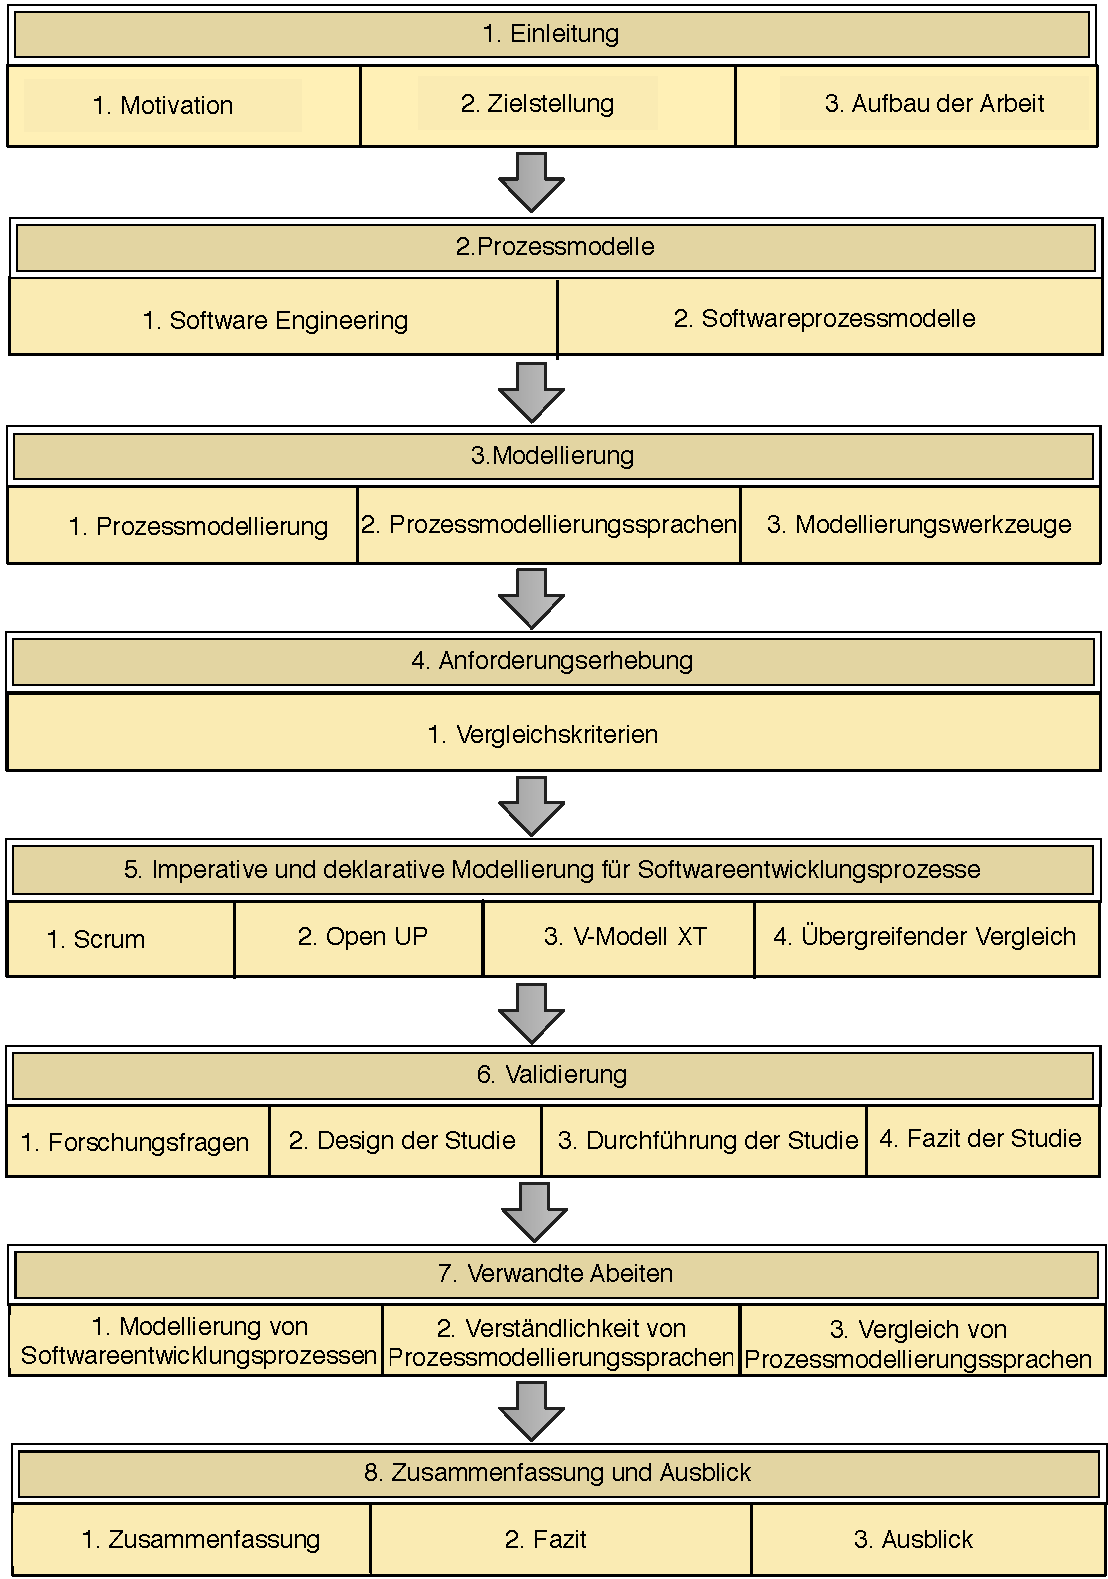
\includegraphics[scale=0.8]{Aufbau} %pdf, jpg, png...
  \caption{Aufbau der Arbeit}
  \label{fig:Aufbau}
\end{center}
\end{figure}


\chapter{Prozessmodelle}\label{sec:chapter2}

In Kapitel 2 werden grundlegende Konzepte des Software Engineering vorgestellt, die notwendig sind, um den Inhalt dieser Arbeit zu verstehen. Zunächst wird in Kapitel 2.1 der Begriff Software Engineering definiert und die Ziele, der Prozess und die Prinzipien des Software Engineering werden erläutert. Weiterhin wird in Kapitel 2.2 der Begriff Softwareentwicklungsprozess erklärt. Hierbei werden Softwareprojekttypen sowie schwergewichtige und leichtgewichtige Prozessmodelle beschrieben. Anschließend gibt es eine Einführung in die drei repräsentativen Softwareentwicklungsprozesse Scrum, Open Unified Process und V-Modell-XT.

\section{Software Engineering}\label{sec:chapter2: Software Engineering}
Heutzutage werden immer mehr Systeme von Software kontrolliert \cite{Puntambekar2007}. Unter Software versteht man laut Duden die "Gesamtheit aller Programme, die auf einem Computer eingesetzt werden können". Das Wort Engineering, welches sich laut Duden von dem lateinischen Wort Ingenium (=[schöpferische] Begabung; Erfindungsgabe) ableitet, wird heutzutage mit Ingenieurwesen, bzw. technische Entwicklung übersetzt. Software Engineering umfasst somit die Gesamtheit der Aktivitäten zur Analyse, Konzeption, Entwicklung und Implementierung einer softwaretechnischen Lösung \cite{Specker1998}.
Software Engineering besteht aus mehreren Schichten (Abbildung \ref{fig:SchichtenSE}):

\begin{figure}[htp]
\begin{center}
  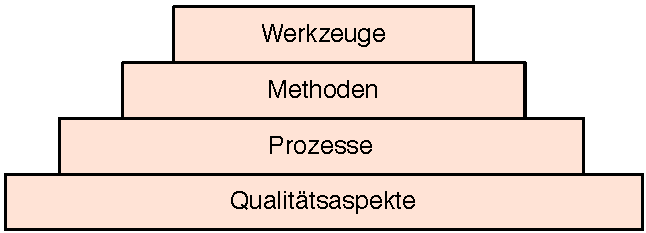
\includegraphics[width=.5\linewidth]{SELayer} %pdf, jpg, png...
  \caption{Schichten des Software Engineering \cite{Puntambekar2007}}
  \label{fig:SchichtenSE}
\end{center}
\end{figure}

Somit ist für Software Engineering in erster Linie in der Schicht Qualitätsaspekte ein diszipliniertes Qualitätsmanagement notwendig. Weiterhin ist eine Prozessschicht vorhanden, um die termingerechte Ablieferung von Software zu gewährleisten. In der Methoden-Schicht wird sodann die Implementierung unter Zuhilfenahme von Anforderungsanalysen, Design und Programmierung durchgeführt. Hierbei werden Werkzeuge zur Automatisierung in Software- Dokumentenprozessen benutzt. Software Engineering stellt somit letztendlich eine Kombination aus Prozessen, Methoden und Tools dar, um eine qualitativ hochwertige Software zu entwickeln \cite{Puntambekar2007}.

\subsection{Ziele, Prozess und Prinzipien des Software Engineering}

Das Hauptziel bei Software Engineering ist, dass die Lösungen mit den Anforderungen übereinstimmen. Vollständige und konsistente Anforderungserhebungen sind, insbesondere für große Systeme, selten. Sowohl die Nutzer, als auch die Entwickler haben ein oftmals unvollständiges Verständnis des eigentlichen Problems und erheben ihre Anforderungen erst während der Entwicklung. Somit muss man mit Änderungen der Anforderungen an ein System während dessen Entwicklung rechnen. Aus diesem Grund ist es wichtig, Ziele beim Software Engineering zu haben, um die Auswirkungen solcher Änderungen einzudämmen \cite{Booch1993}.
Abbildung  \ref{fig:Wuerfel} zeigt die von \cite{ross1975software} definierten Ziele, Prinzipien und den Prozess des Software Engineering, welche nachfolgend genauer erläutert werden: 

\begin{figure}[htp]
\begin{center}
  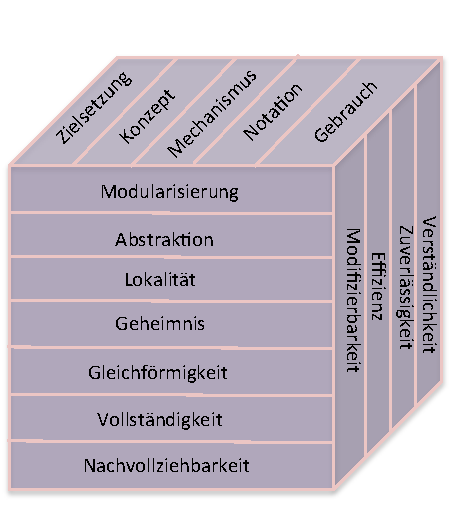
\includegraphics[width=0.6\linewidth]{Wuerfel} %pdf, jpg, png...
  \caption{Ziele, Prozess und Prinzipien des Software Engineering  \cite{ross1975software}}
  \label{fig:Wuerfel}
\end{center}
\end{figure}

\subsubsection{Prinzipien des Software Engineering}


 Das \textit{Modularisierungsprinzip} gibt vor, wie Softwaresysteme am besten strukturiert werden sollen. Das \textit{Abstraktionsprinzip} soll dabei helfen, sich von unwichtigen Details, welche für die zu entwickelnde Lösung irrelevant sind, zu lösen. Das \textit{Lokalitätsprinzip} verlangt das räumlich zusammenhängende Ablegen von zusammengehörenden Informationen. Das \textit{Geheimnisprinzip} bezieht sich auf das Definieren und Durchsetzen von Zugriffsbeschränkungen. Konsistenz wird durch das \textit{Gleichförmigkeitsprinzip} gewährleistet. Durch das \textit{Vollständigkeitsprinzip} wird sichergestellt, dass nichts vergessen wurde. Das Prinzip der \textit{Nachvollziehbarkeit} stellt sicher, dass Informationen, welche zur Überprüfung der Korrektheit benötigt werden detailliert dargelegt werden \cite{ross1975software}.
 
 \subsubsection{Prozess des Software Engineering}

Wie Abbildung  \ref{fig:Wuerfel} entnommen werden kann, besteht der Prozess des Software Engineering aus 5 Schritten: Im ersten Schritt \textit{Zielsetzung} werden die Anforderungen an ein System erhoben. Anschließend erfolgt im Schritt \textit{Konzept} die Ableitung der Software-Architektur, um die zuvor erhobenen Anforderungen zu erfüllen. Des Weiteren werden die Komponenten des Softwaresystems festgelegt. Im dritten Schritt \textit {Mechanismus} erfolgt sodann die Implementierung des Software-Systems. Im darauffolgenden Schritt \textit{Notation} wird die Kommandosprache definiert, die ein Benutzer verwendet, um die Funktionalitäten des Software-Systems aufzurufen. Im letzten Schritt \textit{Gebrauch} muss noch die Bedienung des Systems, z.B. in Form eines Benutzerhandbuches, beschrieben werden \cite{ross1975software}.

  \subsubsection{Ziele des Software Engineering}

\textit{Modifizierbarkeit} ist das wohl schwierigste Ziel des Software Engineering. Hierbei geht es darum, dass es mitunter notwendig wird, Teile des zu entwickelnden Systems zu ändern, während andere Teile unverändert bleiben, aber dennoch das gewünschte neue Ergebnis erreicht wird. Auf die \textit{Effizienz} der jeweiligen Aktivitäten sollte immer geachtet werden, da dieses Ziel des Software Engineering häufig vernachlässigt wird. Bei dem Ziel \textit{Zuverlässigkeit} geht es darum, einerseits Fehler bei der Konzeption, im Design und der Implementierung zu vermeiden andererseits muss auch Fehlverhalten bei der Ausführung und der Leistung verhindert werden \cite{ross1975software}.
 
\section{Softwareentwicklungsprozesse}\label{sec:chapter.2: Softwareentwicklungsprozesse}

Für das Verständnis, die Schaffung oder Unternehmung von etwas Großem, fertigen Menschen in der Regel ein vereinfachtes Bild davon an. Hierfür nehmen sie Maß, fertigen eine Skizze oder einen Plan an oder orientieren sich an einem Vorbild, bzw. bauen sich eines. Dies geschieht normalerweise mit Papier und Schreibzeug, anderen Materialien oder einem Computer. Besonders für die Lösung von komplexen wissenschaftlichen Problemen oder bei großen Konstruktionsaufgaben ist dies unumgänglich \cite{Hesse2008}. \newline
Hierbei stützten sich die Menschen auf Modelle, welche als Stellvertreter für die Sache, die verstanden, geschaffen, unternommen oder betrieben werden soll, angesehen werden kann \cite{Hesse2008}. \newline
Insbesondere die heutzutage von Softwareentwicklern zu erstellenden Softwareprodukte zeichnen sich durch ein hohes Maß an Komplexität und Umfang aus. Neben den Erwartungen von Kunden hinsichtlich Qualität müssen Softwaresysteme ebenfalls termingerecht und innerhalb eines vorgegebenen Budgetrahmens erstellt werden. Effektive und effiziente Softwareentwicklungsprozesse gewinnen somit immer mehr an Bedeutung \cite{Grechenig2010}.
Modell leitet sich von dem lateinischen Begriff  \glqq modelus\grqq \ 
ab und kann mit  \glqq Regel, Form, Muster, Vorbild\grqq \ übersetzt werden \cite{Hesse2008}. 
Der Begriff Prozess stammt von dem lateinischen Wort "processus" ' ab und lässt sich mit "Fortgang oder Verlauf"' übersetzen \cite{koch2011, Staud2006}. \newline 
Ein Softwareprozess ist eine Abfolge von Schritten, welche zur Herstellung von Software notwendig sind \cite{Mishra2012, Stoerrle2005}. Mit Hilfe eines Softwareentwicklungsprozesses lässt sich der organisatorische Rahmen zur Herstellung von Software beschreiben \cite{Koelmel2000}. Ein Softwareentwicklungsprozess stellt somit ein Modell für die Entwicklung eines Softwaresystems dar \cite{Hanser2010}. Die einzelnen Abschnitte eines Softwareprozesses werden hierbei als Phasen bezeichnet \cite{Stoerrle2005}. Diese werden unterschieden in "Planung des Prozesses", "Spezifikation der Anforderungen an das Produkt", Design des Softwareprodukts", "Implementierung" und "Diverse Tests des Softwareprodukts" (siehe Abbildung \ref{fig:SEProzess}).

\begin{figure}[htp]
\begin{center} 
  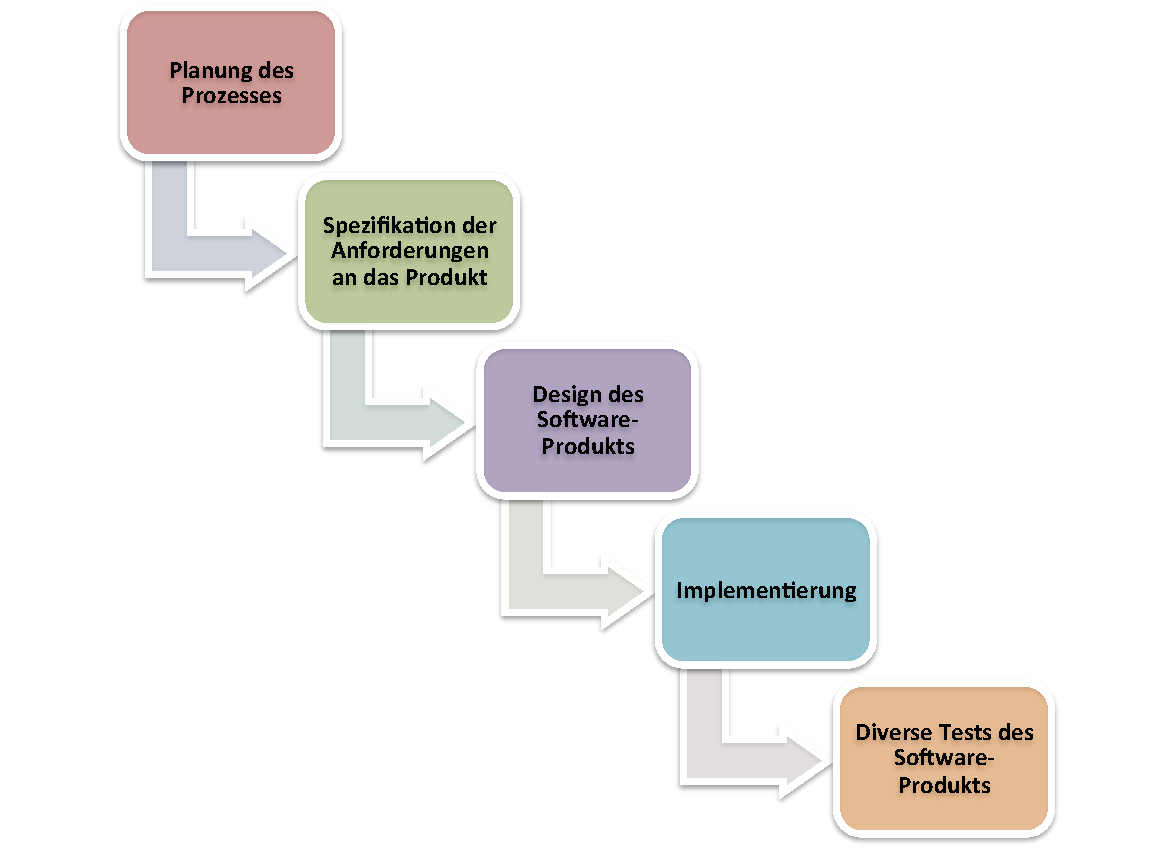
\includegraphics[width= 0.8\linewidth]{Softwareprozess} %pdf, jpg, png...
  \caption{Phasen Softwareprozess nach \cite{Hanser2010}}
  \label{fig:SEProzess}
\end{center}
\end{figure}

In einem Softwareentwicklungsprozess werden nicht nur die durchzuführenden Aktivitäten definiert, sondern auch die Rollen und Qualifikationen der Mitarbeiter, welche die jeweiligen Aktivitäten durchführen sollen, bzw. für diese verantwortlich sind. Des Weiteren werden die während des Entwicklungsprozesses zu erstellenden Dokumente und Unterlagen festgelegt \cite{Hanser2010}.

\subsection{Software-Projekttypen}

Software-Projekte lassen sich in drei Gruppen einteilen (siehe Abbildung \ref{fig:Projekttypen}):
\begin{figure}[htp]
\begin{center}
  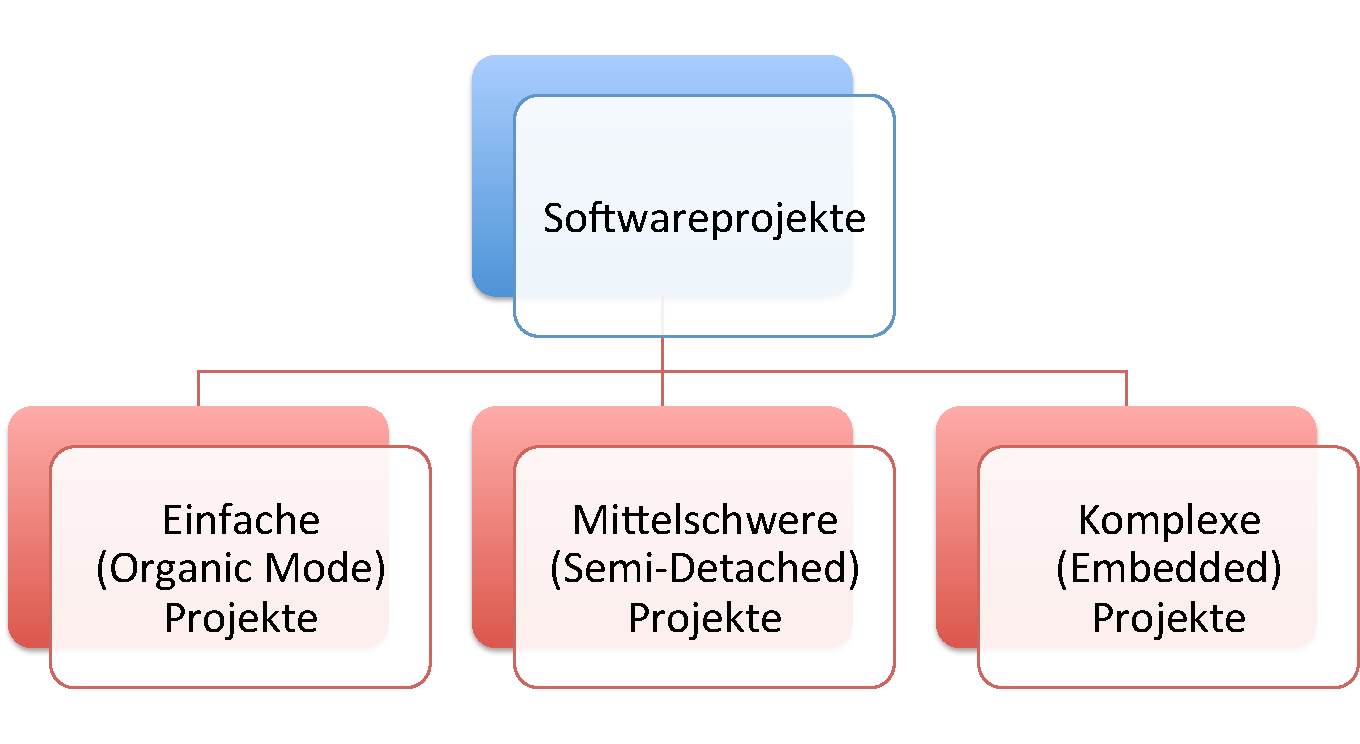
\includegraphics[width= 0.8\linewidth]{Projekttypen} %pdf, jpg, png...
  \caption{Software-Projekttypen nach \cite{Boehm81}}
  \label{fig:Projekttypen}
\end{center}
\end{figure}
Bei den \textit{Einfachen Projekten} sind relativ kleine Teams am Entwicklungsprozess beteiligt und bei den Teammitgliedern besteht räumliche Nähe. Jedes Teammitglied weist eine hohe methodische und fachliche Erfahrenheit auf und kennt sich in dem späteren Einsatzgebiet der Software gut aus. Die Anzahl der Code-Zeilen bei der zu entwickelnden Software ist meist gering \cite{Boehm81, Hanser2010}. \newline
Bei den \textit{Komplexen Projekten} handelt es sich um Software-Projekte, welche in den meisten Fällen stark durch behördliche Auflagen reguliert sind. Die Software muss einerseits eine hohe Zuverlässigkeit aufweisen und andererseits sind nachträgliche Änderungen fast nicht mehr möglich. Im Gegensatz zu den \textit{Einfachen Projekten} ist das Entwicklungsteam hier groß, besteht sowohl aus erfahrenen, als auch aus unerfahrenen Entwicklern und die Anzahl der Code-Zeilen ist ebenfalls groß \cite{Boehm81, Hanser2010}. \newline
Eine Schnittstelle zwischen diesen beiden Projekttypen bilden die \textit{Mittelschweren Projekte}. Hier sind die Software-Entwicklungsteams mittelgroß und bestehen aus erfahrenen und unerfahrenen Mitgliedern. Teilweise sind nicht alle Aspekte des Produktes schon im Vornherein bekannt und die Anzahl der Code-Zeilen ist groß \cite{Boehm81, Hanser2010}.

\subsection{Schwergewichtige und Leichtgewichtige Prozessmodelle}

Aus der eben erfolgten Einteilung von Software-Projekten lässt sich eine Einteilung von Software-Prozessmodellen in \textit{Leichtgewichtige} und \textit{Schwergewichtige Prozessmodelle} ableiten \cite{Hanser2010}. \newline
\textit{Leichtgewichtige Prozessmodelle} eignen sich eher für kleine Teams, bei denen keine detaillierte Anforderungserhebung stattfindet, da die Kommunikation sowohl innerhalb des Teams, als auch mit dem Kunden auf Grund der kleinen Teamgröße gut funktioniert. Da viele Informationen hier informell über kurze Kommunikationswege weitergegeben werden, ist eine ausführliche Dokumentation derer nicht notwendig. \cite{Hanser2010}. \newline
Eine sehr formale und dokumentenlastige Vorgehensweise kommt bei den \textit{Schwergewichtigen Prozessmodellen} zum Einsatz. Es findet eine ausführliche Dokumentation in allen Entwicklungsphasen statt und der Ablauf des Prozesses ist genau vorgegeben. Bei Software-Produkten, welche bei einer möglichen Fehlfunktion Menschenleben in Gefahr bringen, ist beispielsweise eine Vorgehensweise mit einem \textit{Schwergewichtigen Prozessmodell} sinnvoll \cite{Hanser2010}. \newline















\chapter{Modellierung}\label{sec:chapter3}
Kapitel 3 liefert einen Überblick über die Grundlagen der Modellierung. Zunächst werden in Kapitel 3.1 die Grundlagen der Prozessmodellierung erläutert. Hierbei wird auf die Grundsätze ordnungsgemäßer Modellierung eingegangen. Anschließend werden in Kapitel 3.2 Prozessmodellierungssprachen diskutiert. Einerseits werden imperative Modellierungssprachen erklärt und es wird ein kurzer Einblick in die Prozessmodellierungssprache BPMN gegeben. Andererseits werden deklarative Prozessmodellierungssprachen beschrieben und es erfolgt ein Einblick in die deklarative Prozessmodellierungssprache ConDec. In Kapitel 3.3 werden die in dieser Arbeit für die imperative und deklarative Modellierung verwendeten Modellierungswerkzeuge vorgestellt.

\section{Prozessmodellierung}\label{sec:chapter3:Prozessmodellierung}

Prozessmodellierung hat den Zweck, Prozesse zu beschreiben \cite{fahland2010}. Ein Prozessmodell ist eine vereinfachte Darstellung eines Prozesses und besteht aus einer Abfolge von Tätigkeiten, welche chronologisch-sachlogisch angeordnet sind. Der Umfang und Detaillierungsgrad der Prozessmodelle kann sich je nach Zweck und Zielsetzung unterscheiden \cite{koch2011}.

\subsection{Ziele der Prozessmodellierung}
Mit der Modellierung von Prozessen werden verschiedene Ziele verfolgt. Eine erste Übersicht über die Ziele der Prozessmodellierung gibt Abbildung \ref{fig:ZieleProzess} \cite{koch2011}.
\begin{figure}[htp]
\begin{center}
  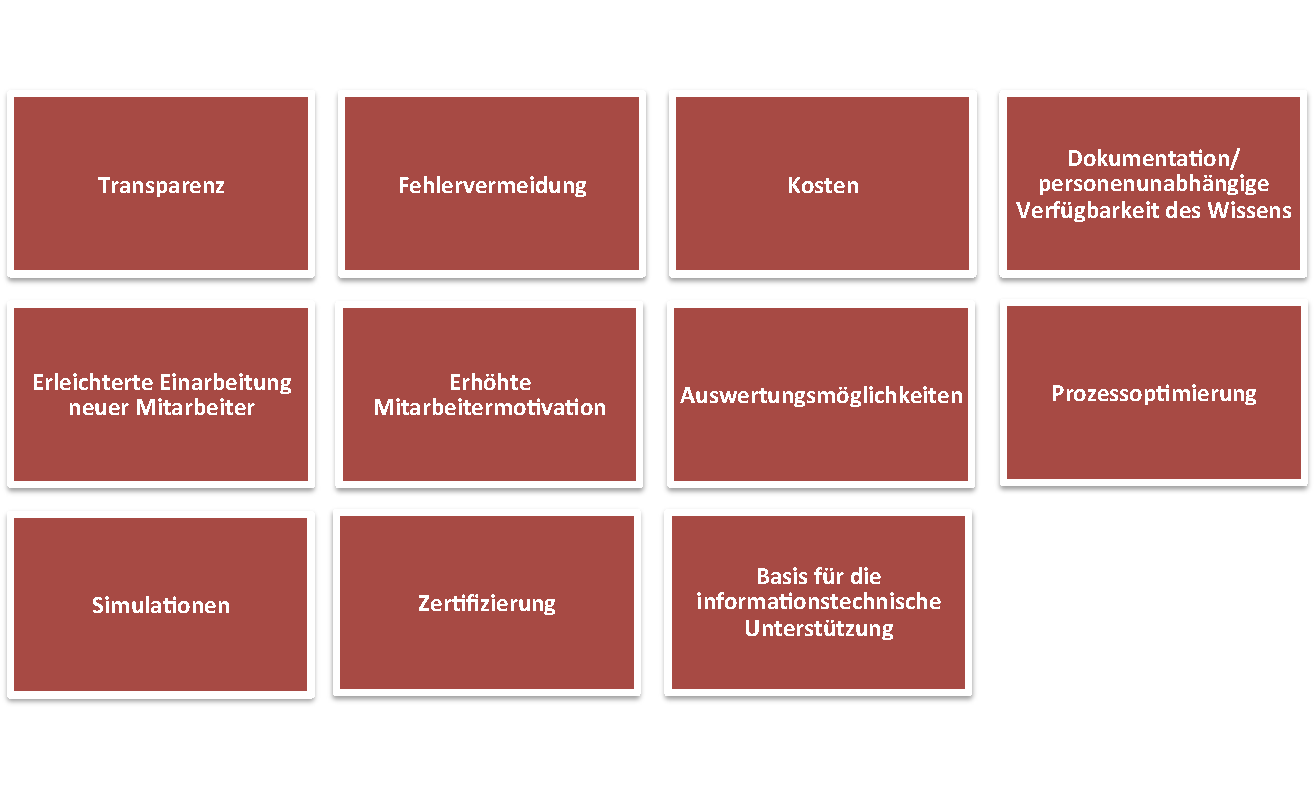
\includegraphics[width=\textwidth]{ZieleProzess} %pdf, jpg, png...
  \caption{Ziele der Prozessmodellierung nach \cite{koch2011}}
  \label{fig:ZieleProzess}
\end{center}
\end{figure}

Bei der \textit{Transparenz} geht es darum, dass alle Beteiligten am Prozess einsehen können, von wem welche Aufgaben durchgeführt werden. Weiterhin verfolgt die Prozessmodellierung das Ziel, durch \textit{Fehlervermeidung} die Qualität, Termintreue und Kundenzufriedenheit zu erhöhen. Durch die Modellierung eines Prozesses kann dieser genau analysiert werden und hierdurch können Einsparungspotenziale von \textit{Kosten} aufgedeckt werden. Indem die Abläufe in einem Unternehmen als Prozesse dargestellt werden, ist es möglich, eine \textit{personenunabhängige Verfügbarkeit des Wissens} zu erreichen, da das Wissen hierdurch allen Personen zugänglich gemacht wird, unabhängig davon, ob sie am Prozess beteiligt sind oder nicht. Die Prozessmodellierung führt zu einer \textit{erleichterten Einarbeitung neuer Mitarbeiter}. Durch die Darstellung der Tätigkeiten der einzelnen Mitarbeiter in Prozessmodellen wird ihnen ihr Beitrag zum Erfolg des Unternehmens vor Augen geführt was eine \textit{erhöhte Mitarbeitermotivation} zur Folge hat. Nach deren Erstellung gibt es verschiedene \textit{Auswertungsmöglichkeiten} für die Prozessmodelle. Durch die Modellierung von Prozessen werden etwaige Schwachstellen, wie z.B. Doppelarbeiten und Prozessverzögerungen offengelegt, wodurch eine \textit{Prozessoptimierung} möglich ist. Mit Hilfe von \textit{Simulationen} der Prozessmodelle lassen sich eventuelle Engpässe rechtzeitig erkennen. Die Voraussetzung für die \textit{Zertifizierung} nach DIN EN ISO 9000:1000 sind Prozessmodelle als Dokumentation. Basis für die Entwicklung von Softwaresystemen bilden Prozessmodelle, weshalb sie als \textit{Basis für die informationstechnische Unterstützung} dienen \cite{koch2011}.

\subsection{Grundsätze ordnungsgemäßer Modellierung}

Bei der Gestaltung eines Modelles sollten grundlegende Prinzipien beachtet werden, um die Qualität eines Modelles zu sichern. Hierfür gibt es die Grundsätze ordnungsgemäßer Modellierung, über deren Prinzipien Abbildung \ref{fig:Prinzipien} einen Überblick gibt  \cite{freund2007}.

\begin{figure}[htp]
\begin{center}
  \includegraphics[scale=0.6]{Prinzipien} %pdf, jpg, png...
  \caption{Grundsatz ordnungsgemäßer Modellierung nach \cite{journals95}}
  \label{fig:Prinzipien}
\end{center}
\end{figure}

Der \textit{Grundsatz der Richtigkeit} besitzt zwei verschiedene Ausprägungen: Eine syntaktische und eine semantische. Die syntaktische \textit{Richtigkeit} eines Modelles wird durch die Einhaltung der Notationsregeln der dem Modell zugrunde liegenden Prozessmodellierungssprache erreicht \cite{journals95, becker2012prozessmanagement}. \newline

Ein Modell wird als semantisch korrekt, oder auch formal korrekt bezeichnet, wenn es dem ihm zugrunde liegenden Metamodell gegenüber vollständig und konsistent ist, d.h. es gibt den abzubildenden Sachverhalt korrekt wieder. Hierbei muss einerseits auf die korrekte Abbildung der Struktur des Metamodelles, als auch des dort beschriebenen Verhaltens geachtet werden \cite{journals95, becker2012prozessmanagement}. \newline


Modelle werden üblicherweise in getrennten Sichten modelliert, um die Komplexität so gering wie möglich zu halten. Beispielsweise werden Prozesse in einem Prozessmodell, die Daten aber in einem Datenmodell modelliert. Werden bei einer Modellierung mehrere Sichten (z.B. Organisationssicht, Datensicht, Funktionssicht) modelliert, müssen diese auch ineinander integriert werden. Beim \textit{Grundsatz des systematischen Aufbau} geht es darum, bei der Modellierung auch auf die anderen Sichten zu achten, um eine spätere konsistente Integration der verschiedenen Sichten zu gewährleisten. Insbesondere ist zu vermeiden, dass die gleichen Informationsobjekte mehrmals mit jeweils verschiedenen Begriffen verwendet werden. Weiterhin sollten die Eingabedaten eines Prozessmodells einen Verweis auf bestehende Datenmodelle enthalten \cite{journals95, freund2007, becker2012prozessmanagement,koch2011}.\newline

Der \textit{Grundsatz der Relevanz} besagt, dass alle Elemente und Verknüpfungen eines Modells, ohne die der Nutzen des Modells sinken würde, für die Modellierung relevant sind \cite{journals95, reinshagen2009}. Auf der anderen Seite sollten aber auch nur diejenigen Teile der Realität in das Modell aufgenommen werden, die wirklich notwendig sind. Es sollte somit darauf geachtet werden, nur so viele Informationen ins Modell zu bringen wie minimal benötigt werden \cite{journals95, freund2007,reinshagen2009}.\newline


Durch den \textit{Grundsatz der Klarheit} soll sichergestellt werden, dass das Modell für den Adressaten verständlich ist. Es muss also bei der Modellierung auf Strukturiertheit, Verständlichkeit und Anschaulichkeit geachtet werden. Insbesondere sollte das Modell ohne besondere methodische Kenntnisse verständlich sein. Somit sollte die Modellierung entweder von links nach rechts oder von oben nach unten verlaufen, wobei darauf zu achten ist, dass sich Flusslinien und Kanten hierbei so wenig wie möglich überkreuzen. Weiterhin sollte die Anzahl der Elemente auf das Nötigste reduziert werden. Vor allem die Anzahl an Verzweigungen innerhalb eines Prozessmodells wirkt sich negativ auf die Verständlichkeit von Prozessmodellen aus. Ebenso hat eine hohe Anzahl von Verbindungen zwischen Aktivitäten einen negativen Einfluss auf das Verständnis \cite{leimeister2012,journals95, freund2007,reinshagen2009, becker2012prozessmanagement,koch2011,bpm07,thesis_maja}.\newline

Der \textit{Grundsatz der Wirtschaftlichkeit} sagt aus, dass die Modellierung kosteneffektiv durchzuführen ist \cite{leimeister2012}. Es gilt also abzuwägen, ob der Aufwand, der für die Modellierung notwendig ist, auch einen entsprechenden Nutzen bringt \cite{freund2007, journals95}.\newline

Wird in unterschiedlichen Modellen der gleiche Sachverhalt abgebildet, so sollten letztendlich auch vergleichbare Modelle entstehen, unabhängig von der verwendeten Modellierungssprache. Dies besagt der \textit{Grundsatz der Vergleichbarkeit}. Insbesondere ist auf einen einheitlichen Abstraktionsgrad der Prozessmodelle zu achten \cite{leimeister2012, journals95, freund2007,reinshagen2009}.\newline


\section{Prozessmodellierungssprachen}\label{sec:chapter3:Prozessmodellierungssprachen}

Die Modellierung eines Prozesses mit natürlicher Sprache bringt einige Nachteile mit sich, wie z.B. fehlende Eindeutigkeit, schwer zu überprüfende Vollständigkeit und teilweise Widersprüche. Mögliche Folgen davon können unterschiedliche Interpretationen, Missverständnisse und falsche Schlussfolgerungen sein. Eine reine Beschreibung der Prozessmodelle mit mathematischen Modellen und Formalismen führt jedoch oftmals zu einer Verminderung der intuitiven Verständlichkeit der Prozessmodelle. Aus diesem Grund ist es sinnvoll den Prozess graphisch als Diagramm mit einer Prozessmodellierungssprache darzustellen, da diese eine Schnittstelle zwischen formaler Exaktheit und intuitiver Verständlichkeit bilden \cite{thomas2009,kircher2006}.  \newline
Hierfür existieren eine Reihe verschiedener Prozessmodellierungssprachen, deren Vor- und Nachteile intensiv diskutiert werden. Ein viel erörterter Unterschied ist der zwischen imperativen und deklarativen Prozessmodellierungssprachen \cite{fahland2010}. \newline
Die ursprüngliche Unterscheidung zwischen imperativen und deklarativen Sprachen stammt aus der Programmierung. Während imperative Programmierung angibt, "Wie etwas zu tun ist", folgt deklarative Programmierung dem Ansatz \grqq Sag was benötigt wird und lass das System herausfinden, wie es erreicht werden kann\grqq \ \cite{pichler2012}.

\subsection{Imperative Modellierung}
Imperative Programmierung wird als zustandsbehaftete Programmierung bezeichnet, da das  Ergebnis einer Komponente nicht nur von ihren Argumenten abhängt, sondern auch von internen Parametern, was auch als ihr \grqq Zustand\grqq \  bezeichnet wird \cite{fahland2010}.  \newline
Ähnlich wie die imperative Programmierung, folgt auch die imperative Modellierung einem \grqq Inside-Out-Ansatz \grqq. Alle Ausführungsalternativen eines Prozesses sind somit in diesem spezifiziert und alle weiteren Ausführungsalternativen müssen explizit hinzugefügt werden. Bei der imperativen Modellierung werden Prozesse mit Operatoren und elementaren Aktivitäten modelliert. Hierbei können Sequenz, Parallelität und Synchronisation beschrieben werden \cite{kaschek1998}. Bei einer imperativen Modellierungssprache liegt der Fokus auf den ständigen Veränderungen der Prozess-Objekte.

\subsubsection {BPMN}

Die \textit{Business Process Modelling Notation (BPMN)} wurde von der \textit{Business Process Management Initiative} entwickelt und 2004 veröffentlicht. Seit 2005 wird sie von der \textit{Object Management Group} standardisiert und weiterentwickelt \cite{krallmann2013}.
Die BPMN Notationselemente lassen sich anhand der fünf Kategorien \textit{Swimlanes}, \textit{Flussobjekte}, \textit{verbindende Objekte}, \textit{Daten} und \textit{Artefakte} einteilen. Abbildung \ref{fig:BPMN} zeigt die Einteilung und die wichtigsten Prozess-Elemente von BPMN, welche nachfolgend genauer erläutert werden \cite{gpfert2012}. \newline

\begin{figure}[htp]
\begin{center}
  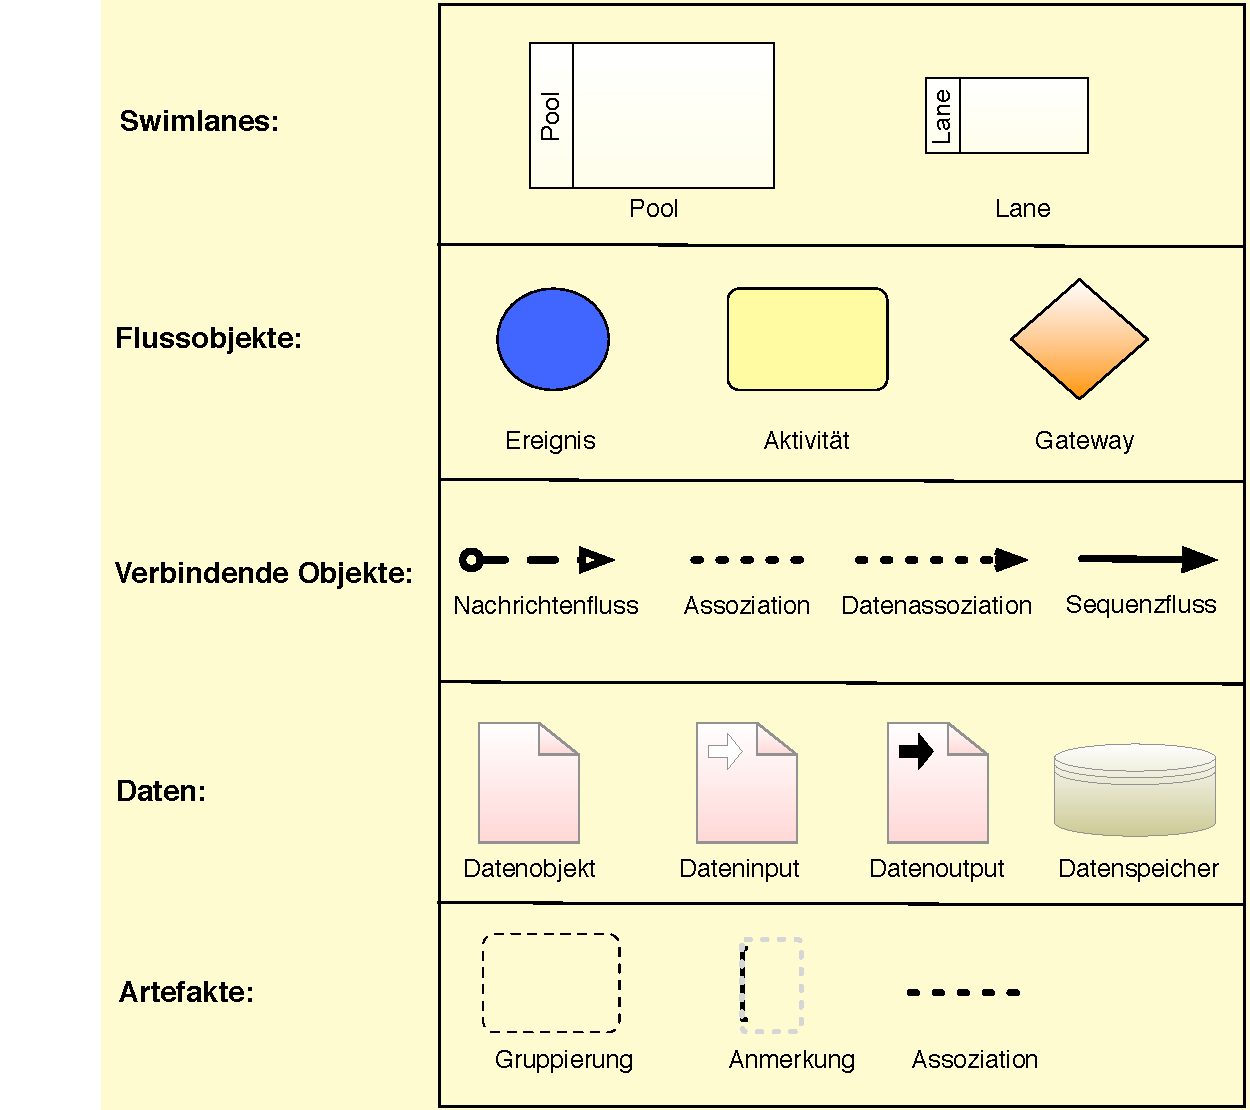
\includegraphics[scale=0.6]{BPMN} %pdf, jpg, png...
  \caption{BPMN-Elemente Übersicht nach \cite{gpfert2012}}
  \label{fig:BPMN}
\end{center}
\end{figure}

In der Kategorie \textbf{Swimlanes} befinden sich \textit{Pools} und \textit{Lanes}. \textit{Pools} stellen eine Art Container für den Prozess dar. Ein \textit{Pool} ist ein Prozessteilnehmer. Ein Prozessteilnehmer ist z.B. eine Organisationseinheit oder eine selbstständige Geschäftseinheit. Werden in einem Prozessmodell mehrere \textit{Pools} verwendet, so können hiermit Kollaborationen zwischen verschiedenen Prozessteilnehmern dargestellt werden. Ein \textit{Pool} kann in mehrere \textit{Lanes} unterteilt werden. \textit{Lanes} können untergeordnete Organisationseinheiten, Partnerrollen (z.B. Vertrieb, Projektleitung, Marketing) oder auch verschiedene Bestandteile eines Systems sein \cite{gpfert2012, pitschke2010, allweyer2013}. \newline
 \textit{Ereignisse}, \textit{Aktivitäten} und \textit{Gateways} befinden sich in der Kategorie \textbf{Flussobjekte}.
Start und Ende von Prozessen werden in BPMN durch \textit{Ereignisse} beschrieben. Diese werden in  \textit{Startereignisse} und \textit{Endereignisse} unterschieden und geben somit den Beginn und das Ende eines Prozesses an. Weiterhin gibt es auch noch \textit{Zwischenereignisse}. Hierdurch können beispielsweise Pausen im Prozess modelliert werden. Der Prozess stoppt in diesem Fall solange, bis ein bestimmtes Ereignis eintritt \cite{allweyer2013}. \newline
\textit{Aktivitäten} stellen Arbeitseinheiten dar und sind ein Oberbegriff für Aufgaben, Unterprozesse und Aufruf-Aktivitäten. Aufgaben sind Tätigkeiten, welche nicht weiter unterteilt werden können, während ein Unterprozess eine Aufgabe darstellt, welche in weitere Tätigkeiten unterteilt werden kann. Beschriftet werden sie mit einer Objekt-Verb-Verbindung (z.B. Lieferung überprüfen) \cite{gpfert2012}. \newline
Mit Hilfe von \textit{Gateways} lässt sich der Prozessablauf kontrollieren und steuern, da durch diese Verzweigungen und Zusammenführungen von Sequenzflüssen dargestellt werden. \cite{gpfert2012, allweyer2013}. Hierbei werden \textit{Exklusive Gateways} zur Modellierung alternativer Pfade, \textit{Parallele Gateways} zur Modellierung parallel ablaufender Pfade, \textit{Inklusive Gateways} zur Modellierung der Auswahl eines oder mehrerer Pfade und \textit{Komplexe Gateways} zur Modellierung komplexer Regeln bei Verzweigungen und Zusammenführungen, unterschieden \cite{allweyer2013}.\newline 

\begin{figure}[H]
\begin{center}
  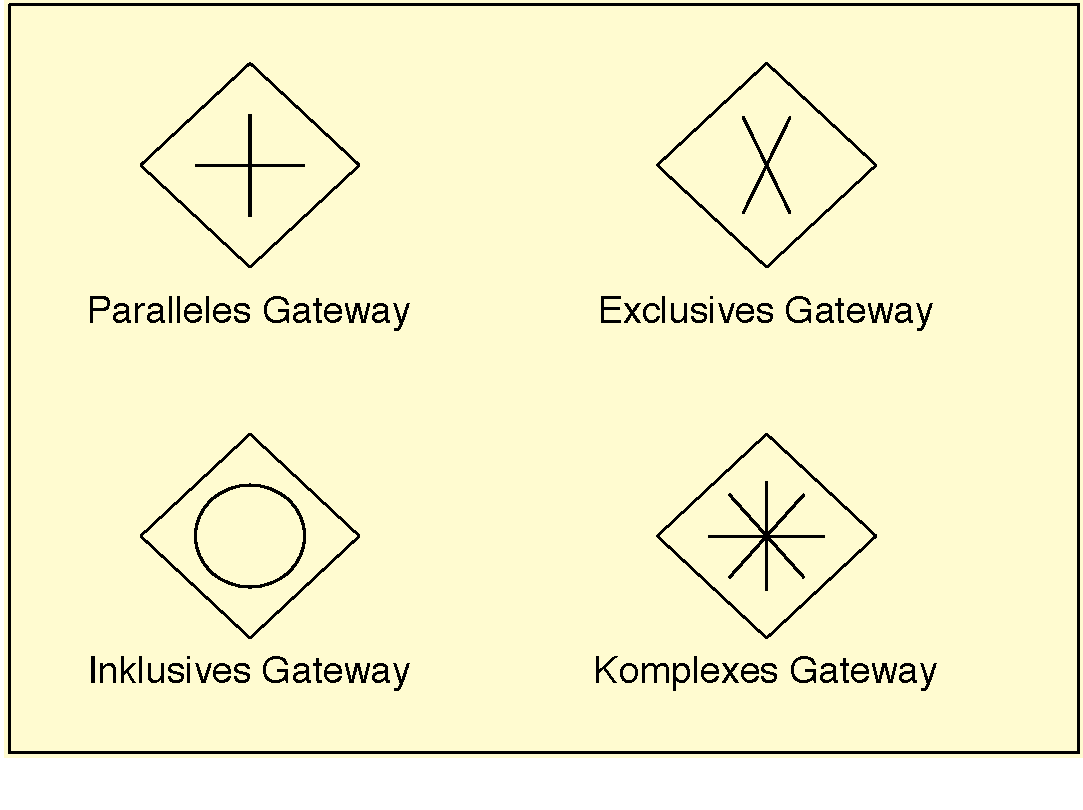
\includegraphics[scale=0.5]{gates} %pdf, jpg, png...
  \caption{BPMN-Gateways}
  \label{fig:gates}
\end{center}
\end{figure} 


\textit{Nachrichtenfluss}, \textit{Assoziation}, \textit{Datenassoziation} und \textit{Sequenzfluss} bilden zusammen die Kategorie \textbf{Verbindende Objekte}. Ein \textit{Nachrichtenfluss} wird dazu verwendet, den Nachrichtenfluss zwischen zwei getrennten Prozessteilnehmern, z.B. aus zwei verschiedenen Unternehmen, darzustellen. Mit Hilfe einer \textit{Assoziation} können Daten, Text und andere Artefakte mit Flussobjekten verknüpft werden. Hiermit werden die Ein- und Ausgabe von Aktivitäten aufgezeigt. Ein \textit{Sequenzfluss} dient dazu, die Reihenfolge der Aktivitäten im Prozess festzulegen \cite{white2004introduction}. \newline
In der Kategorie \textbf{Daten} gibt es \textit{Datenobjekte}, \textit{Dateninput}, \textit{Datenoutput} und \textit{Datenspeicher}. \textit{Datenobjekte} geben hierbei an, welche Daten von den Aktivitäten benötigt werden, bzw. von diesen erzeugt werden \cite{white2004introduction}. Sie stellen somit Informationen dar, welche durch den Prozess fließen. Bei einem  \textit{Dateninput} handelt es sich um einen externen Input für den ganzen Prozess, der von einer Aktivität gelesen wird. Ein \textit{Datenoutput} hingegen wird als Ergebnis eines ganzen Prozesses erzeugt. Somit handelt es sich bei \textit{Dateninput}, bzw. \textit{Datenoutput} um Eingangs-, bzw. Ausgangsprozessschnittstellen \cite{bpmnposter}. Ein \textit{Datenspeicher} kann für den indirekten Austausch von Daten zwischen zwei verschiedenen Prozessteilnehmern verwendet werden. Hierfür ist es notwendig, dass beide Prozessteilnehmer Zugriff auf den \textit{Datenspeicher} haben \cite{allweyer2013}.\newline
Die Kategorie \textbf{Artefakte} beinhaltet \textit{Gruppierung}, \textit{Anmerkung} und \textit{Assoziation}. Diese ergänzen den Prozess um zusätzliche Informationen, haben jedoch keinerlei Einfluss auf diesen \cite{gpfert2012}. Eine \textit{Gruppierung} kann hierbei zur Dokumentation oder für Analysezwecke benutzt werden. Durch \textit{Anmerkungen} können dem Leser zusätzliche Informationen in Textform bereitgestellt werden \cite{white2004introduction}. Mit Hilfe einer \textit{Assoziation} lassen sich Datenobjekte mit Aktivitäten und Prozessen verknüpfen \cite{bpmnposter}. \newline
 Eine Übersicht über alle Elemente der BPMN Notation kann Anhang A entnommen werden.\newline





\subsection{Deklarative Modellierung}

 Die deklarative Modellierung folgt im Gegensatz zur imperativen Modellierung einem \grqq Outside-In-Ansatz\grqq \ \cite{lichtenegger2012}. Das heißt, deklarative Sprachen legen den Ablauf nicht im Vorhinein fest \cite{pichler2012} und sie sind somit sehr flexibel \cite{reichert2012}. Zu Beginn befinden sich nur die Aktivitäten im Prozessmodell und erlauben jegliches Ausführungsverhalten. Erst wenn Constraints zum Modell hinzugefügt werden, werden schrittweise Ausführungsalternativen verworfen \cite{pichler2012}. Constraints lassen sich hierbei in die beiden verschiedenen Kategorien \textbf{Ausführungsconstraints} und \textbf{Terminierungsconstraints} einteilen. Die Ausführungsconstraints geben Einschränkungen für die Ausführung von Aktivitäten an. Hierbei kann es sich z.B. um die Anzahl möglicher Ausführungen für eine Aktivität oder eine Mindestzeitverzögerung zwischen zwei Aktivitäten handeln. Terminierungsconstraints hingegen führen auf, wann eine korrekte Terminierung (Beendigung) des Prozesses möglich ist. Es kann hier z.B. vorgeschrieben werden, dass eine Aktivität mindestens einmal ausgeführt werden muss oder dass der Aktivität A Aktivität B folgen muss. Bevor dies nicht geschehen ist, kann der Prozess nicht korrekt enden \cite{reichert2012}.  Abbildung \ref{fig:Dec} zeigt ein Beispiel für ein deklaratives Prozessmodell. Es besteht aus den drei Aktivitäten A, B und C sowie aus zwei Constraints:  Das Constraint zwischen A und B legt fest, dass der Aktivität B die Aktivität A vorausgehen muss und das Constraint bei Aktivität C legt fest, dass diese mindestens einmal ausgeführt werden muss, aber beliebig oft durchgeführt werden kann. Abgesehen von diesen Bedingungen, können die Aktivitäten sowohl beliebig oft als auch in beliebiger Reihenfolge ausgeführt werden. Es wäre z.B. [A,B,C,C,A,B,C] eine korrekte Ausführungsreihenfolge. Die Ausführungsreihenfolgen [C,B,C,A] oder [A,B,A,B] wären jedoch inkorrekt, da bei der ersten Ausführungsreihenfolge B vor A ausgeführt wird und somit das Constraint zwischen diesen beiden Aktivitäten verletzt würde. Bei der zweiten Ausführungsreihenfolge wird Aktivität C nicht bearbeitet, wodurch das Constraint bei Aktivität C verletzt wird \cite{pesic2006}. \newline

\begin{figure}[H]
\begin{center}
  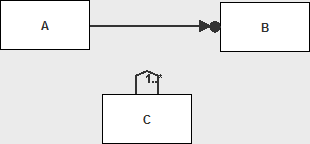
\includegraphics[scale=0.8]{DecProcessModel} %pdf, jpg, png...
  \caption{Deklarativer Beispiel-Prozess \cite{pesic2006}}
  \label{fig:Dec}
\end{center}
\end{figure} 

\subsubsection{ConDec}

Die deklarative Modellierungssprache ConDec wurde erstmals unter dem Namen DecSerFlow veröffentlicht \cite{fahland2010}. Mit ConDec lassen sich einerseits sehr strenge Modelle erstellen, welche den gesamten Prozess im Detail vorgeben und andererseits sehr leichtgewichtige Modelle, welche zwar angeben, welche Arbeit getan werden muss, aber nicht wie sie ausgeführt werden muss \cite{pesic2006}. \newline
In ConDec gibt es die vier verschiedenen Arten von Contraints: \textit{Existenz}, \textit{Choice}, \textit{Relation} und \textit{Negation}. Tabelle \ref{tab:tab3} zeigt die Bedeutung der verschiedenen Constraints. \newline

\begin{table}
\begin{tabular}{|p{0.5\textwidth}|p{0.5\textwidth}|}
\hline
\textbf{Constraint} & \textbf{Erläuterung}\\
\hline
Existenz Constraints & Ein-stellige Kardinalitäts-Constraints. Sie geben an, wie oft eine Aktivität ausgeführt werden kann bzw. muss.\\
\hline
Choice Constraints & N-stellige Constraints. Sie geben die Notwendigkeit der Ausführung von Aktivitäten an, die zu einer Reihe möglicher Alternativen gehören, unabhängig von anderen Constraints. \\
\hline
Relation Constraints & Zwei-stellige Constraints. Sie geben vor, dass eine gewisse Aktivität ausgeführt werden muss falls eine andere Aktivität ausgeführt wird. Es können auch qualitative zeitliche Constraints zwischen diesen beiden Aktivitäten verlangt werden.\\
\hline
Negation Constraints & Stellt die negative Version der Relation Constraints dar. Sie verbieten explizit die Ausführung einer gewissen Aktivität, wenn eine andere Aktivität ausgeführt wird.\\
\hline
 \end{tabular}
  \caption{Constraints ConDec \cite{pesic2006}}
\label{tab:tab3}
 \end{table}
 Eine Übersicht über die genaue Notation von ConDec ist in Anhang B verfügbar.


\section{Modellierungswerkzeuge}\label{sec:chapter3:Modellierungswerkzeuge}
Ein Modellierungswerkzeug ist ein Softwaresystem, mit dessen Hilfe sich Prozessmodelle erstellen  lassen. Teilweise bietet ein Modellierungswerkzeug noch weitere Funktionen wie z.B. das Ausführen und Monitoring der Prozesse, Simulationen und die Analyse von Prozessmodellen an. Die Ausführung der Prozessschritte kann hierbei durch die jeweilige Person, welche für die Aktivität zuständig ist, ausgeführt werden. Für die Prozessmodellierung in der vorliegenden Arbeit kommt das Modellierungswerkzeug Signavio für die imperative Modellierung mit BPMN und Declare für die deklarative Modellierung mit ConDec zum Einsatz. Diese beiden Modellierungswerkzeuge werden nachfolgend vorgestellt \cite{gadatsch2012}.

\subsection{Signavio}

Bei Signavio handelt es sich um ein webbasiertes Prozessmodellierungstool, welches auch das kollaborative Modellieren von Prozessen mit den Modellierungsstandards BPMN und EPC zulässt. Ein großer Vorteil von Signavio besteht darin, dass es nicht auf dem Rechner installiert werden muss, sondern direkt im Web-Browser ausgeführt werden kann. Die Prozessmodelle werden in einem zentralen Repository gespeichert und sind für die Benutzer entsprechend ihren Zugriffsrechten aufrufbar. Prozessmodelle besitzen alle eine eigene eindeutige URL und können über diese im Web-Browser aufgerufen werden. Hierbei wird auch gleich die Modellierungsumgebung mitgeladen und kann somit im Web-Browser ausgeführt werden \cite{quteprints}. Abbildung \ref{fig:Signavio} zeigt den \textit{Signavio Process Editor}.

\begin{figure}[H]
\begin{center}
  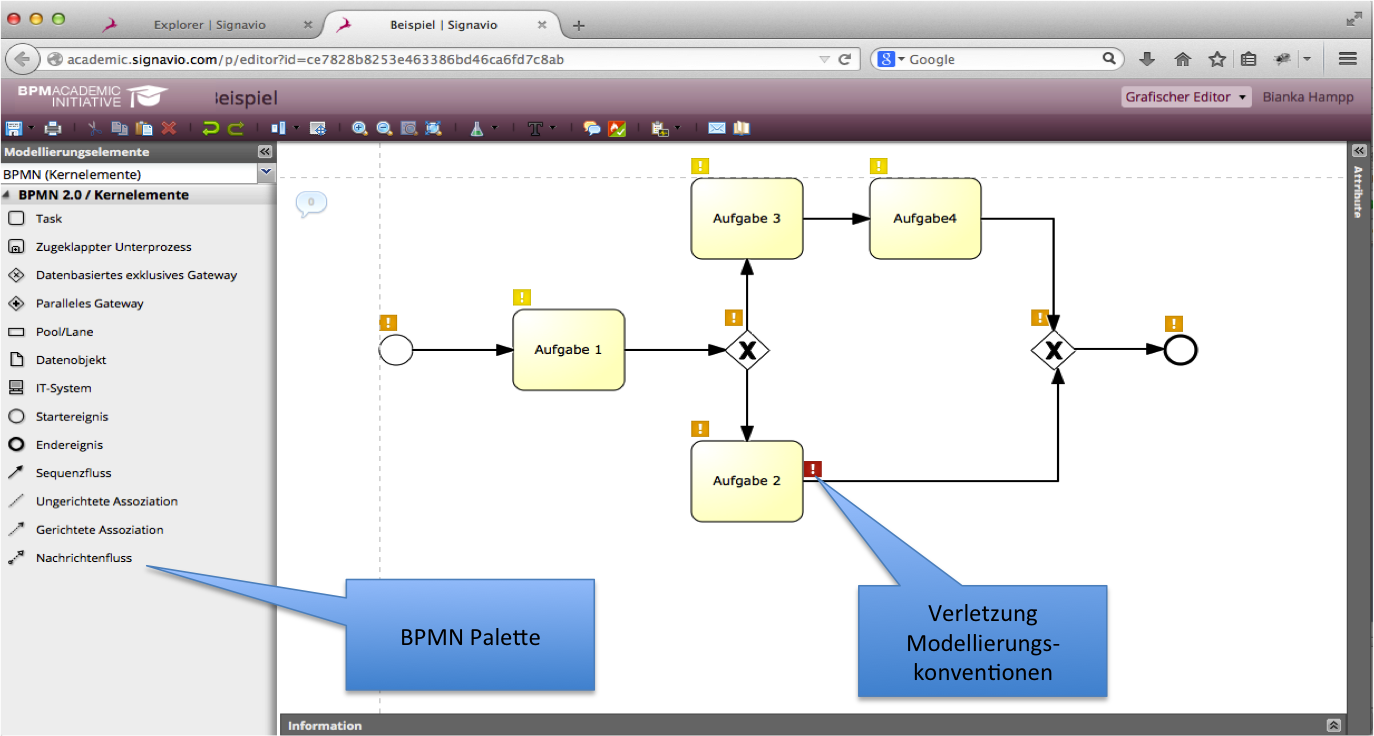
\includegraphics[scale=0.6]{Signavio} %pdf, jpg, png...
  \caption{Siganvio Process Editor (Screenshot Siganvio)}
  \label{fig:Signavio}
\end{center}
\end{figure} 

Links in Abbildung \ref{fig:Signavio} ist die BPMN Palette zu sehen. Die einzelnen Elemente können per \textit{Drag and Drop} in das Arbeitsdokument gezogen werden. Signavio verfügt über eine automatische Überprüfung von Modellierungskonventionen. Durch diese ist es möglich, das Modell auf die Einhaltung von Modellierungsrichtlinien, wie z.B. Notationsumfang, Benennung, Prozessstruktur und Diagrammlayout zu überprüfen. Die Modelle können alle als PDF exportiert werden. \newline
In Abbildung \ref{fig:Simulation} ist die Simulations-Sicht von Signavio zu sehen. Hier kann der Benutzer den Prozessablauf simulieren. Dies kann einerseits mit Benutzerinteraktion Schritt für Schritt erfolgen oder auch im Ganzen durch den Simulator gesteuert werden, wobei XOR-Verzweigungen nach wie vor vom Benutzer ausgewählt werden müssen.
\begin{figure}[H]
\begin{center}
  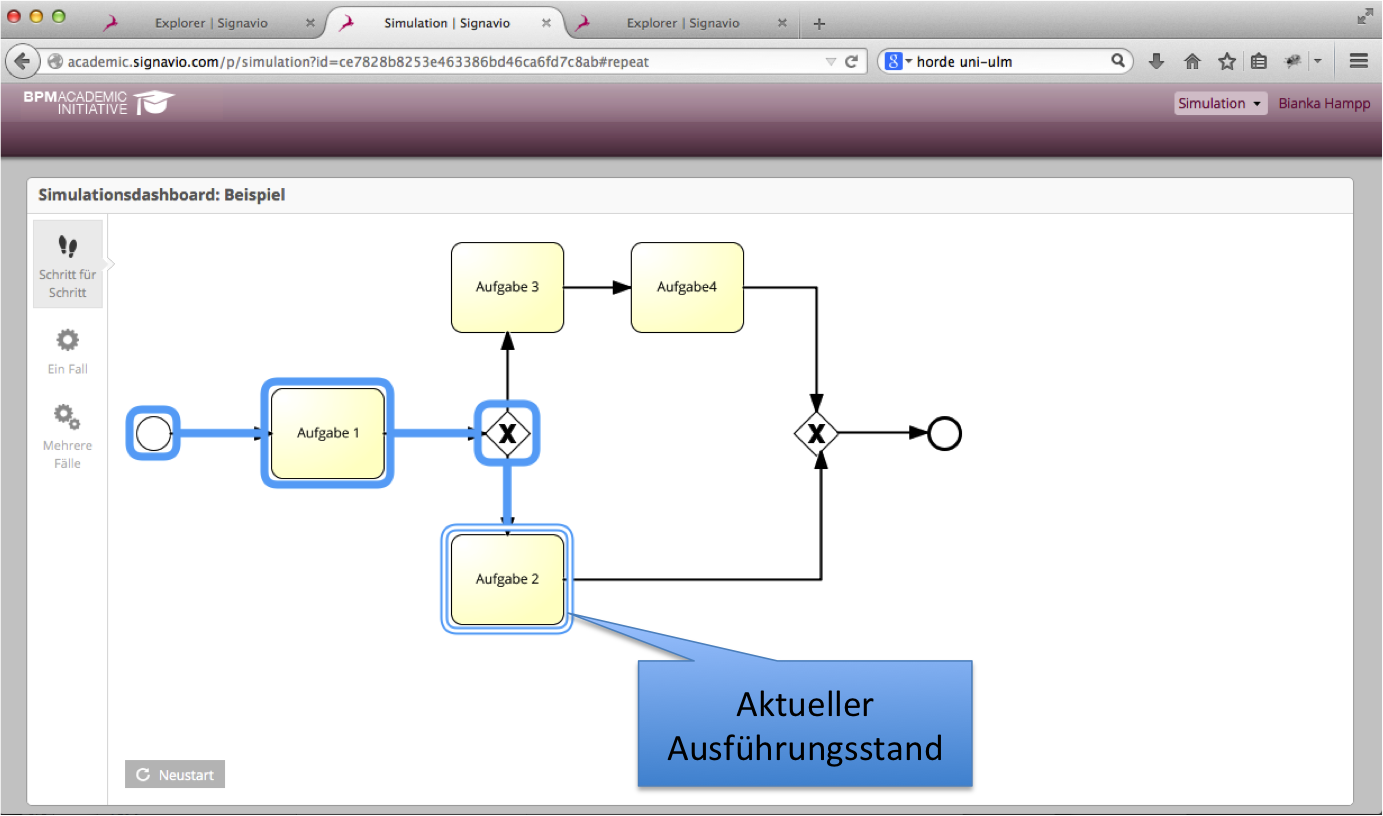
\includegraphics[scale=0.6]{Simulation} %pdf, jpg, png...
  \caption{Siganvio Simulation (Screenshot Signavio)}
  \label{fig:Simulation}
\end{center}
\end{figure} 



\subsection{Declare}

Declare wurde als Constraint-basiertes Workflow-Management-System entwickelt. Es wird für die Entwicklung von Prozessmodellen, welche auf deklarativen Sprachen basieren, benutzt. Declare bietet die folgenden Funktionen an \cite{pesic2007declare}:
\begin {itemize}
\item Modellentwicklung
\item Modellüberprüfung (Suche nach Fehlern in Modellen)
\item automatisierte Modellausführung
\item Modelle können zur Laufzeit geändert werden
\item Analyse der bereits ausgeführten Prozesse
\item Prozess Dekomposition
\end {itemize}

Abbildung \ref{fig:Declare} zeigt die Systemarchitektur von Declare.

\begin{figure}[H]
\begin{center}
  \includegraphics[scale=0.8]{Declare} %pdf, jpg, png...
  \caption{Declare Systemarchitektur nach \cite{pesic2007declare}}
  \label{fig:Declare}
\end{center}
\end{figure} 

Hieraus wird ersichtlich, dass \textit{Declare} mit den beiden Systemen \textit{YAWL} und \textit{ProM} kooperiert. Bei \textit{YAWL} handelt es sich um ein Workflow-Management System, welches auf strukturierte Workflows spezialisiert ist. Dies wirkt sich auf die Zusammenarbeit mit \textit{Declare} in der Art aus, dass die strukturierten Teile des Prozesses von \textit{YAWL} abgehandelt werden, während die unstrukturierten Teile von \textit{Declare} übernommen werden. Bei \textit{ProM} handelt es sich um ein Prozess-Mining-Tool. Hier werden bereits ausgeführte Prozesse von \textit{Declare} analysiert und darauf aufbauend werden dem Nutzer während der Prozessausführung Empfehlungen gegeben \cite{pesic2007declare}. \newline
Weiterhin besteht \textit{Declare} selbst aus drei Komponenten \textit{Framework}, \textit{Designer} und \textit{Worklist}.  Beim \textit{Designer} handelt es sich um ein Modellierungstool, welches für Systemeinstellungen und die Prozessmodell-Entwicklung verwendet wird (Abbildung \ref{fig:Designer}). Das \textit{Framework} ist für das Prozess-Enactment (Prozessbereitstellung) zuständig. Außerdem übernimmt es die Kommunikation mit \textit{YAWL} und \textit{ProM} und das Ändern der Prozessmodelle zur Laufzeit (Abbildung \ref{fig:Framework}). Die Prozessausführung wird von \textit{Worklist} durchgeführt. Hier können die Nutzer ihre zuvor erstellten Prozesse ausführen und können die von \textit{ProM} erstellten Empfehlungen sehen (Abbildung \ref{fig:Worklist}). Alle Modelle können als Bilddateien exportiert werden \cite{pesic2007declare}.



\begin{figure}[H]
\begin{center}
  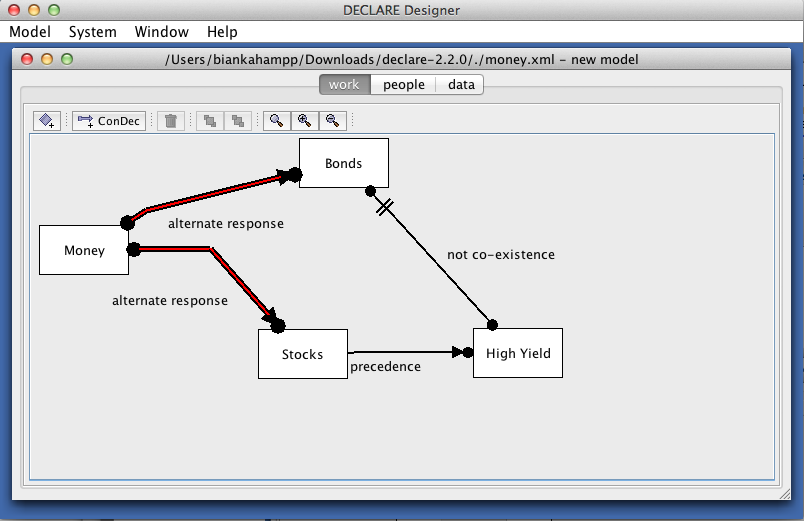
\includegraphics[scale=0.4]{Designer} %pdf, jpg, png...
  \caption{Declare Designer (Screenshot aus Declare)}
  \label{fig:Designer}
\end{center}
\end{figure} 


\begin{figure}[H]
\begin{center}
  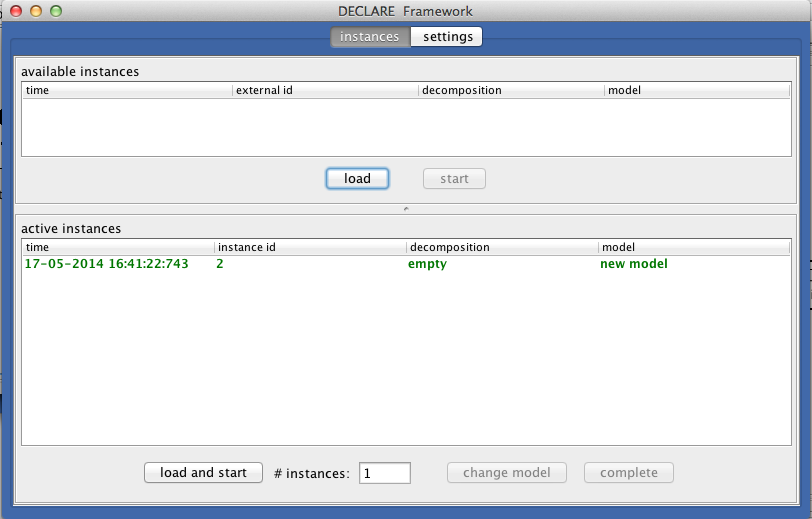
\includegraphics[scale=0.4]{Framework} %pdf, jpg, png...
  \caption{Declare Framework (Screenshot aus Declare)}
  \label{fig:Framework}
\end{center}
\end{figure} 

\begin{figure}[H]
\begin{center}
  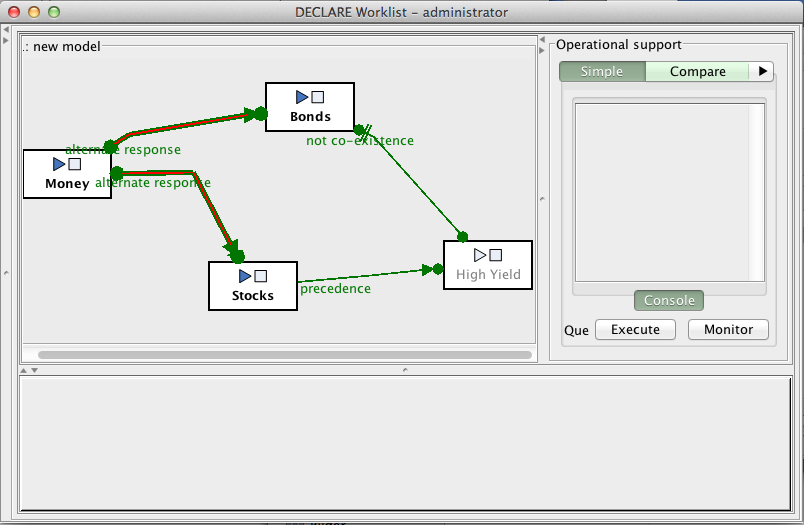
\includegraphics[scale=0.4]{Worklist} %pdf, jpg, png...
  \caption{Declare Worklist (Screenshot aus Declare)}
  \label{fig:Worklist}
\end{center}
\end{figure} 





 










\chapter{Modellierungswerkzeuge}\label{sec:chapter4}
Dieses Kapitel stellt die in dieser Arbeit für die Prozessmodellierung benutzten Modellierungswerkzeuge vor. Nach einer kurzen allgemeinen Einführung in Modellierungswerkzeuge, wird das Modellierungswerkzeug Signavio vorgestellt, welches zur imperativen Modellierung von Prozessen mit BPMN in dieser Arbeit herangezogen wird. Anschließend erfolgt eine Einführung in das Modellierungswerkzeug Declare, mit welchem die deklarativen Prozessmodelle in der Prozessmodellierungssprache ConDec in der vorliegenden Arbeit erstellt werden. 

\section{Modellierungswerkzeuge}\label{sec:chapter4:Modellierungswerkzeuge}
Ein Modellierungswerkzeug ist ein Softwaresystem, mit dessen Hilfe sich Prozessmodelle erstellen, ausführen und monitoren lassen. Teilweise bietet ein Modellierungswerkzeug noch weitere Funktionen wies z.B. Simulationen und die Analyse von Prozessmodellen an. Die Ausführung der Prozessschritte kann hierbei durch die jeweilige Person, welche für die Aktivität zuständig ist ausgeführt werden. Für die Prozessmodellierung in der vorliegenden Arbeit kommt das Modellierungswerkzeug Signavio für die imperative Modellierung mit BPMN und Declare für die deklarative Modellierung mit ConDec zum Einsatz. Diese beiden Modellierungswerkzeuge werden nachfolgend vorgestellt \cite{gadatsch2012}.

\subsection{Signavio}

Bei Signavio handelt es sich um ein webbasiertes Prozessmodellierungstool, welches auch das kollaborative Modellieren von Prozessen mit den Modellierungsstandards BPMN und EPC zulässt. Der Vorteil von Signavio besteht darin, dass es nicht auf dem Rechner installiert werden muss, sondern direkt im Web-Browser ausgeführt werden kann. Die Prozessmodelle werden in einem zentralen Repository gespeichert und sind für die Benutzer entsprechend ihren Zugriffsrechten aufrufbar. Prozessmodelle besitzen alle eine eigene eindeutige URL und können über diese im Web-Browser aufgerufen werden. Hierbei wird auch gleich das Modellierungswerkzeug Signavio mitgeladen und kann somit im Web-Browser ausgeführt werden \cite{quteprints}. \newline
Abbildung \ref{fig:Signavio} zeigt den \textit{Signavio Process Editor}.
\begin{figure}[H]
\begin{center}
  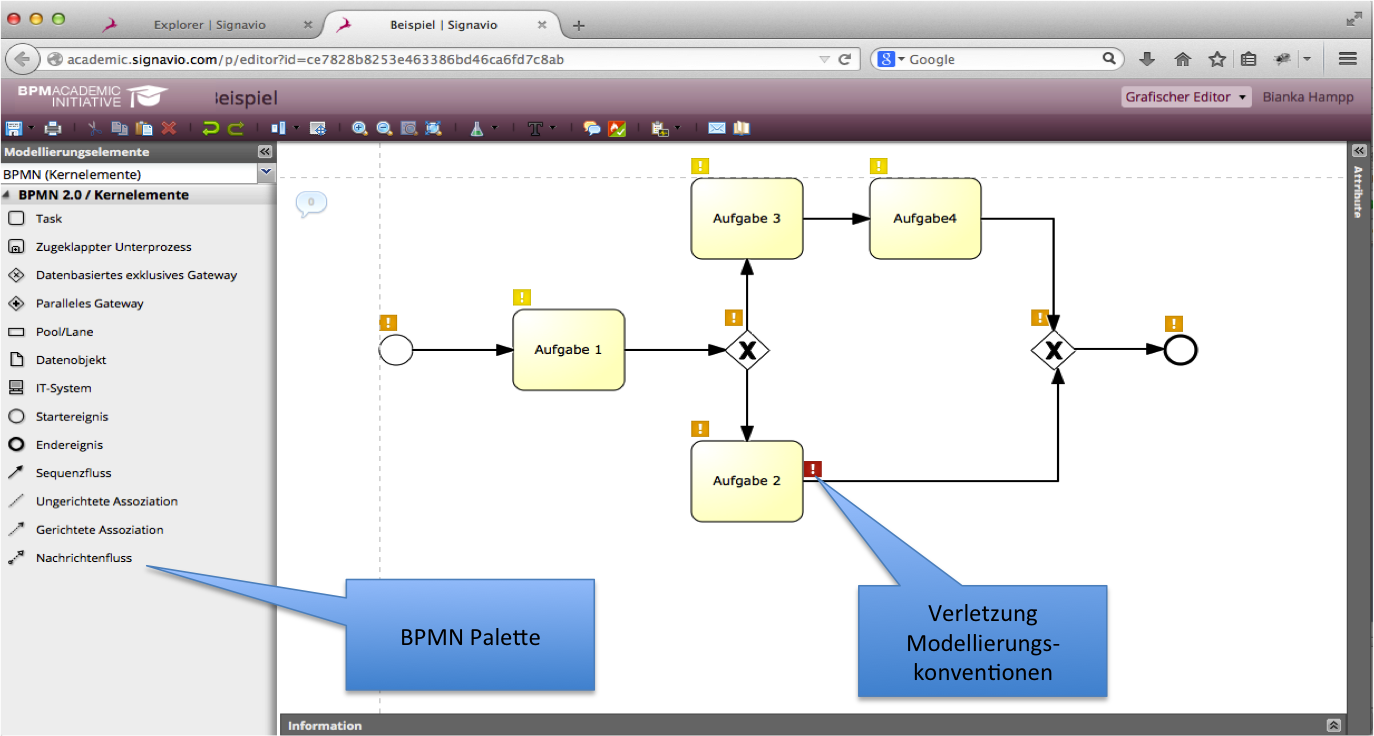
\includegraphics[scale=0.6]{Signavio} %pdf, jpg, png...
  \caption{Siganvio Process Editor}
  \label{fig:Signavio}
\end{center}
\end{figure} 
Links ist die BPMN Palette zu sehen. Die einzelnen Elemente können per \textit{Drag and Drop} in das Arbeitsdokument gezogen werden. Signavio verfügt über Modellierungskonventionen. Mit diesen ist es  möglich, das Modell auf die Einhaltung von Modellierungsrichtlinien, wie z.B. Notationsumfang, Benennung, Prozessstruktur und Diagrammlayout zu überprüfen. Die Modelle können alle als PDF exportiert werden. \newline
In Abbildung \ref{fig:Simulation} ist die Simulations-Sicht von Signavio zu sehen. Hier kann der Benutzer den Prozessablauf simulieren. Dies kann einerseits mit Benutzerinteraktion Schritt für Schritt erfolgen oder auch im Ganzen durch den Simulator gesteuert wobei XOR-Verzweigungen nach wie vor vom Benutzer ausgewählt werden müssen.
\begin{figure}[H]
\begin{center}
  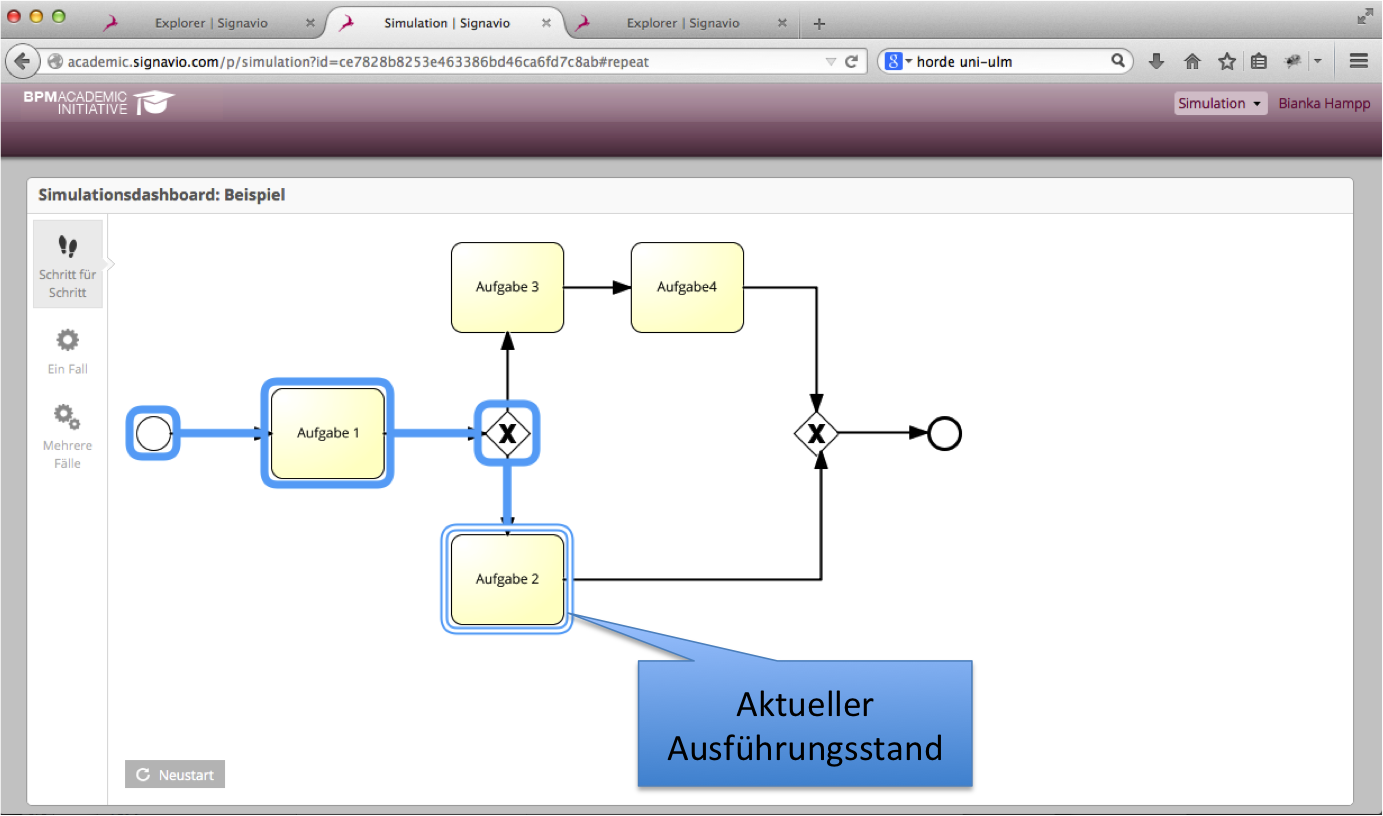
\includegraphics[scale=0.6]{Simulation} %pdf, jpg, png...
  \caption{Siganvio Simulation}
  \label{fig:Simulation}
\end{center}
\end{figure} 



\subsection{Declare}

Declare wurde als Constraint-basiertes Workflow-Management-System entwickelt. Es wird für die Entwicklung von Prozessmodellen, welche auf deklarativen Sprachen basieren, benutzt. Declare bietet die folgenden Funktionen an:
\begin {itemize}
\item Modellentwicklung
\item Modellüberprüfung (Suche nach Fehlern in Modellen)
\item automatisierte Modellausführung
\item wechselnde Modelle zur Laufzeit
\item Analyse der bereits durchgeführten Prozesse
\item Prozess Dekomposition
\end {itemize}

Abbildung \ref{fig:Declare} zeigt die Systemarchitektur von Declare.

\begin{figure}[H]
\begin{center}
  \includegraphics[scale=0.8]{Declare} %pdf, jpg, png...
  \caption{Declare Systemarchitektur}
  \label{fig:Declare}
\end{center}
\end{figure} 

Hieraus wird ersichtlich, dass \textit{Declare} mit den beiden Systemen \textit{YAWL} und \textit{ProM} kooperiert. Bei \textit{YAWL} handelt es sich hierbei um ein Workflow-Management System, welches auf strukturierte Workflows spezialisiert ist. Dies wirkt sich auf die Zusammenarbeit mit \textit{Declare} in der Art aus, dass die strukturierten Teile des Prozesses von \textit{YAWL} abgehandelt werden, während die unstrukturierten Teile von \textit{Declare} übernommen werden. Bei \textit{ProM} handelt es sich um ein Prozess-Mining-Tool. Hier werden bereits ausgeführte Prozesse von \textit{Declare} analysiert und darauf aufbauend werden dem Nutzer während der Prozessausführung Empfehlungen gegeben \cite{pesic2007declare}. \newline
Weiterhin besteht \textit{Declare} selbst aus drei Komponenten \textit{Framework}, \textit{Designer} und \textit{Worklist}.  Beim \textit{Designer} handelt es sich um ein Modellierungstool, welches für Systemeinstellungen und die Prozessmodell-Entwicklung verwendet wird (Abbildung \ref{fig:Designer}). Das \textit{Framework} ist für das Prozess-Enactment zuständig. Außerdem übernimmt es die Kommunikation mit \textit{YAWL} und \textit{ProM} und das Ändern der Prozessmodelle zur Laufzeit (Abbildung \ref{fig:Framework}). Die Prozessausführung wird von \textit{Worklist} durchgeführt. Hier können die Nutzer ihre zuvor erstellten Prozesse ausführen und können die von \textit{ProM} erstellten Empfehlungen sehen (Abbildung \ref{fig:Worklist}). Alle Modelle können als Bilddateien exportiert werden.



\begin{figure}[H]
\begin{center}
  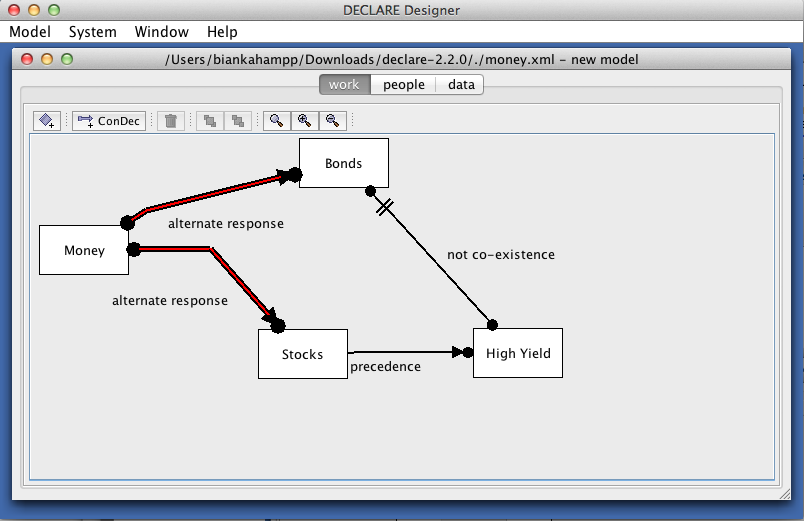
\includegraphics[scale=0.4]{Designer} %pdf, jpg, png...
  \caption{Declare Designer}
  \label{fig:Designer}
\end{center}
\end{figure} 


\begin{figure}[H]
\begin{center}
  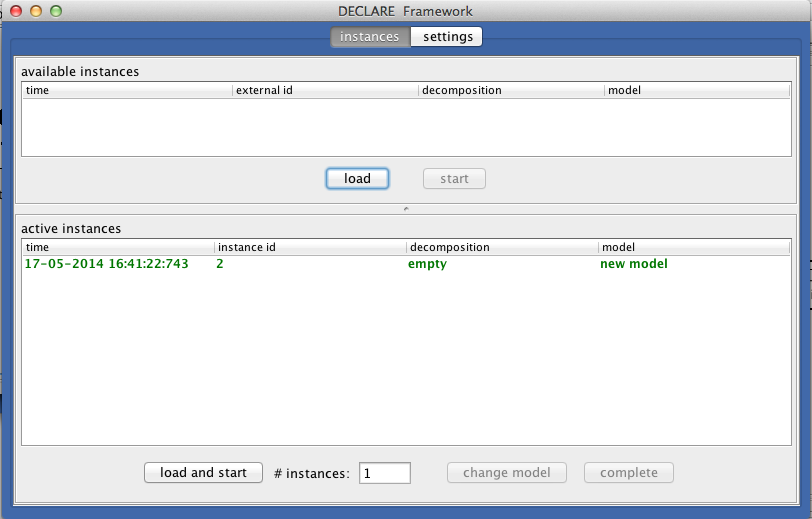
\includegraphics[scale=0.4]{Framework} %pdf, jpg, png...
  \caption{Declare Framework}
  \label{fig:Framework}
\end{center}
\end{figure} 

\begin{figure}[H]
\begin{center}
  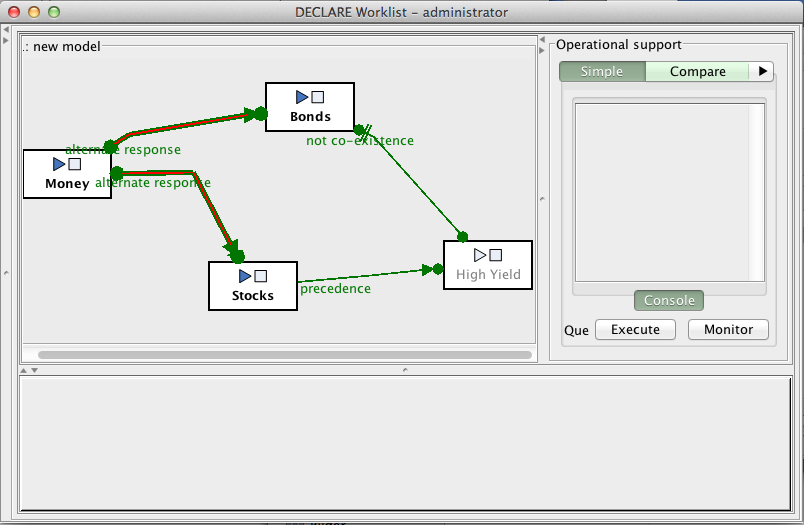
\includegraphics[scale=0.4]{Worklist} %pdf, jpg, png...
  \caption{Declare Worklist}
  \label{fig:Worklist}
\end{center}
\end{figure} 





\chapter{Anforderungserhebung}\label{sec:chapter5}
In diesem Kapitel werden die Anforderungen an den in Kapitel 6 folgenden Vergleich der imperativen und deklarativen Modellierung für SE-Prozessmodelle erhoben.

\section{Vergleichskriterien}\label{sec:chapter5:Vergleichskriterien}

Bisher gibt es nur wenige Arbeiten, welche sich mit deklarativen Prozessmodellierungssprachen und insbesondere mit dem Vergleich von imperativen und deklarativen Prozessmodellierungssprachen beschäftigen. Aus diesem Grund soll in der vorliegenden Arbeit ein Vergleich zwischen deklarativen und imperativen Prozessmodellierungssprachen im Kontext von Software-Engineering Prozessmodellen durchgeführt werden. Hierbei sollen die Unterschiede und Ähnlichkeiten der beiden Prozessmodellierungssprachen herausgearbeitet und deren Eignung für die Modellierung von unterschiedlich großen Prozessmodellen beurteilt werden. Weiterhin sollen die Stärken und Grenzen der beiden Modellierungssprachen aufgezeigt werden und es soll dadurch herausgefunden werden, ob eine der beiden Modellierungssprachen über eine bessere Eignung zur Modellierung verfügt als die andere \cite{list2006evaluation}.\newline
Hierfür sollen die imperativen und deklarativen Prozessmodelle, welche für die drei Software-Engineering Prozessmodelle Scrum, Open Up und V-Modell-XT erstellt werden im Hinblick auf verschiedene Vergleichskriterien untersucht werden. Da es sich bei Scrum um ein leichtgewichtiges Software-Engineering Prozessmodell, beim V-Modell XT um ein schwergewichtiges Software-Engineering Prozessmodell und bei Open Up um ein Software-Engineering Prozessmodell handelt, welches sich in der Mitte zwischen leichtgewichtig und schwergewichtig befindet, eignen sich diese drei besonders gut, zum Vergleichen der imperativen und deklarativen Modellierung für unterschiedlich große Prozessmodelle. Außerdem liegen den in imperativer und deklarativer Modellierungssprache zu erstellenden Prozessmodellen so jeweils die gleichen Metamodelle zugrunde, was eine objektive Bewertung für den Vergleich gewährleistet \cite{list2006evaluation}.  

\subsection{Erfüllung der Modellierungsgrundsätze}
Es sollen die imperativen und deklarativen Modellierungssprachen im Hinblick auf deren Erfüllung der in Kapitel 3.1.1 vorgestellten \textit{Grundsätze ordnungsgemäßer Modellierung} untersucht werden, da durch deren Einhaltung die Qualität, Klarheit und Konsistenz der Prozessmodelle gesichert wird \cite{freund2007}. Somit lässt sich hierdurch die Eignung der beiden Prozessmodellierungssprachen sehr gut überprüfen. Denn falls eine von beiden Prozessmodellierungssprachen die Modellierungsgrundsätze wesentlich schlechter einhalten kann, als die andere, so ist sie zum Modellieren deutlich weniger geeignet, da die hierdurch entstandenen Prozessmodelle geringere Qualität, Klarheit und Konsistenz aufweisen. Hierfür werden nachfolgend die erstellten Prozessmodelle auf \textit{Klarheit}, \textit{Richtigkeit}, \textit{Wirtschaftlichkeit}, \textit{Relevanz}, \textit{Vergleichbarkeit} und \textit{systematischen Aufbau} verglichen. Hierfür werden nachfolgend für jeden Modellierungsgrundsatz verschiedene Kriterien festgelegt, mit deren Hilfe die Einhaltung der Modellierungsgrundsätze für die jeweilige Modellierungssprache überprüft wird. \newline

\subsubsection{Richtigkeit}
Die Richtigkeit der Prozessmodelle soll verglichen werden. Hierbei soll die semantische und syntaktische Richtigkeit der Prozessmodelle untersucht werden. \newline
Bei der semantischen Korrektheit der Prozessmodelle wird verglichen in wie weit die mit deklarativer bzw. imperativer Prozessmodellierungssprache erstellten Prozessmodelle dem zugrunde liegenden Metamodell gegenüber vollständig und konsistent sind. Denn falls wesentliche Aspekte des Metamodells nicht darstellbar sind, leidet der Nutzen des Prozessmodells erheblich. Es wird somit überprüft, ob eine der beiden Prozessmodellierungssprachen die Struktur des Metamodells und das dort beschriebe Verhalten besser abbildet, als die andere. Insbesondere wird hier untersucht, ob es Grenzen in der Darstellbarkeit der abzubildenden Aspekte des Metamodells gibt \cite{journals95, becker2012prozessmanagement}. \newline
Die sysntaktische Korrektheit wird dahingegend untersucht, ob sich die jeweiligen Modelle unter Einhaltung der Modellierungsregeln der jeweiligen Prozessmodellierungssprache erstellen lassen. Dies wird mit Hilfe der Modellierungstools Signavio und Declare durchgeführt. Beide Programme verfügen über eine automatische Überprüfung der syntaktischen Korrektheit der dort erstellten Modelle. \newline


\subsubsection{Systematischer Aufbau}
Um den systematischen Aufbau der imperativen und deklarativen Prozessmodelle zu vergleichen, werden die Prozessmodelle dahingehend untersucht, in wie weit sie die Integration anderer Sichten in das Prozessmodell unterstützen und sie Verweise auf bestehende Datenmodelle zulassen. Da nicht alle Informationen, wie z.B. Daten und Funktionen in einem Prozessmodell abgebildet werden können, ist die Integration anderer Sichten in das Prozessmodell sehr wichtig, um wirklich alle Informationen aus dem Metamodell abbilden zu können. Hier können Rückschlüße auf die Eignung zur Modellierung gezogen werden und eventuelle Grenzen der Prozessmodellierungssprache aufgezeigt werden \cite{journals95, freund2007, becker2012prozessmanagement,koch2011}.

\subsubsection{Relevanz}
Beim Vergleich der Relevanz der Prozessmodelle werden die mit BPMN bzw. ConDec modellierten Prozessmodelle dahingehend verglichen in wie weit es möglich ist die Prozessmodelle mit den minimal relevanten Informationen zu erstellen. Es soll also untersucht werden, ob bei einer der beiden Prozessmodellierungssprachen mehr Informationen im Prozessmodell abgebildet werden müssen, als bei der anderen, um die Qualität des Prozessmodells zu sichern \cite{journals95, freund2007,reinshagen2009}. 

\subsubsection{Wirtschaftlichkeit der Prozessmodelle}
Hier soll untersucht werden, ob sich der Aufwand für die Modellierung bei den beiden Modellierungssprachen erheblich voneinander unterscheidet, da wenn die Erstellung eines Prozessmodells mit einem zu hohen Aufwand für die Erstellung verbunden ist, obwohl der spätere Nutzen des Prozessmodells erheblich geringer ist, ist die Modellierung nicht sinnvoll. Hier kann die Eignung zur Modellierung der Prozessmodellierungssprachen sehr gut verglichen werden, denn falls der Aufwand für die Modellierung für eine der beiden Prozessmodellierungssprachen weitaus höher ist, als für die andere, eignet sich die Prozessmodellierungssprache mit dem sehr viel höherem Aufwand nicht für die Modellierung \cite{freund2007, journals95, leimeister2012}.

\subsubsection{Klarheit}
Die Prozessmodelle, welche jeweils in imperativer und deklarativer Prozessmodellierungssprache erstellt werden, sollen im Hinblick auf ihre Klarheit untersucht werden. Hierbei soll festgestellt werden, ob es wesentliche Unterschiede bei der Verständlichkeit der Prozessmodelle gibt, wenn diese in imperativer, bzw. deklarativer Prozessmodellierungssprache erstellt wurden. Denn fehlende Verständlichkeit eines Prozessmodells führt dazu, dass das Prozessmodell wenig Nutzen bringt. Insbesondere soll hier bei den imperativen Modellen die Anzahl an Verbindungen bzw. bei den deklarativen Modellen die Anzahl an Constraints zwischen Aktivitäten verglichen werden, da sich diese mit steigender Anzahl negativ auf die Verständlichkeit auswirken.\newline
Hier soll auch insbesondere die Anzahl unterschiedlicher Gateways/Constraints betrachtet werden.  Da alle Gateways in BPMN und alle Constraints in ConDec eine unterschiedliche Sematik haben und diese jeweils verstanden werden muss, kann sich eine hohe Anzahl an verschieden Gateways, bzw. Constraints negtiv auf die Verständlichkeit auswirken. Auch wird hier bei ConDec noch die Komplexität der Constraints betrachtet. Denn Existenz-Constraints haben eine geringere Komplexität als Relation Constraints.\newline
Weiterhin soll hier untersucht werden, ob es wesentliche Unterschiede in der Verständlichkeit der imperativen und deklarativen Prozessmodelle gibt, in Abhängigkeit der Größe des zugrunde liegenden Software Engineering Prozessmodells. Hierbei kann die Eignung der jeweiligen Modellierungssprache sehr gut festgestellt werden, da sie im Falle von schwerer/fehlender Verständlichkeit nicht zum Modellieren geeignet ist. Falls es Unterschiede in der Verständlichkeit der Prozessmodelle in Abhängigkeit der Größe des zugrunde liegenden Metamodells gibt, lassen sich hierbei Rückschlüsse auf die Eignung der Prozessmodellierungssprache in Bezug auf große/kleine Metamodelle ziehen \cite{leimeister2012,journals95, freund2007,reinshagen2009, becker2012prozessmanagement,koch2011,bpm07,thesis_maja}.


\subsubsection{Vergleichbarkeit}
Bei der Vergleichbarkeit der Prozessmodelle wird untersucht, ob die in imperativer, bzw. deklarativer Prozessmodellierungssprache erstellten Prozessmodelle, welchen die gleichen Metamodelle zugrunde liegen, trotzdem vergleichbare Prozessmodelle darstellen. Es wird hier somit insbesondere untersucht, ob die Abstraktionsgrade der Prozessmodelle sich wesentlich voneinander unterscheiden. Weiterhin wird die Vergleichbarkeit in Bezug auf das Ausführungsverhalten der imperativen und deklarativen Prozessmodelle durch Ausführung der Modelle in den Modellierungstools Siganvio und Declare nach der Modellierung überprüft. Hier werden die möglichen Pfade im jeweiligen Modell durchlaufen und somit wird sichergestellt, dass das Verhalten der Modelle gleich ist. Außerdem wird hier die Größe der jeweiligen Prozessmodelle als Vergleichskriterium herangezogen. Hier wird die Anzahl der notwendigen Elemente zur Darstellung des Prozessmodells verglichen. Es soll festgestellt werden, ob bei Verwendung einer imperativen oder deklarativen Prozessmodellierungssprache wesentlich mehr Elemente zur Darstellung des gleichen Prozesses notwendig sind indem die Anzahl der verwendeten Aktivitäten und Patterns verglichen wird \cite{leimeister2012, journals95, freund2007,reinshagen2009}.

Eine Übersicht über die Modellierungsgrundsätze und die jeweiligen Vergleichskriterien bietet Abbildung \ref{fig:TabelleKriterien}.

\begin{figure}[!htbp]
\begin{center}
  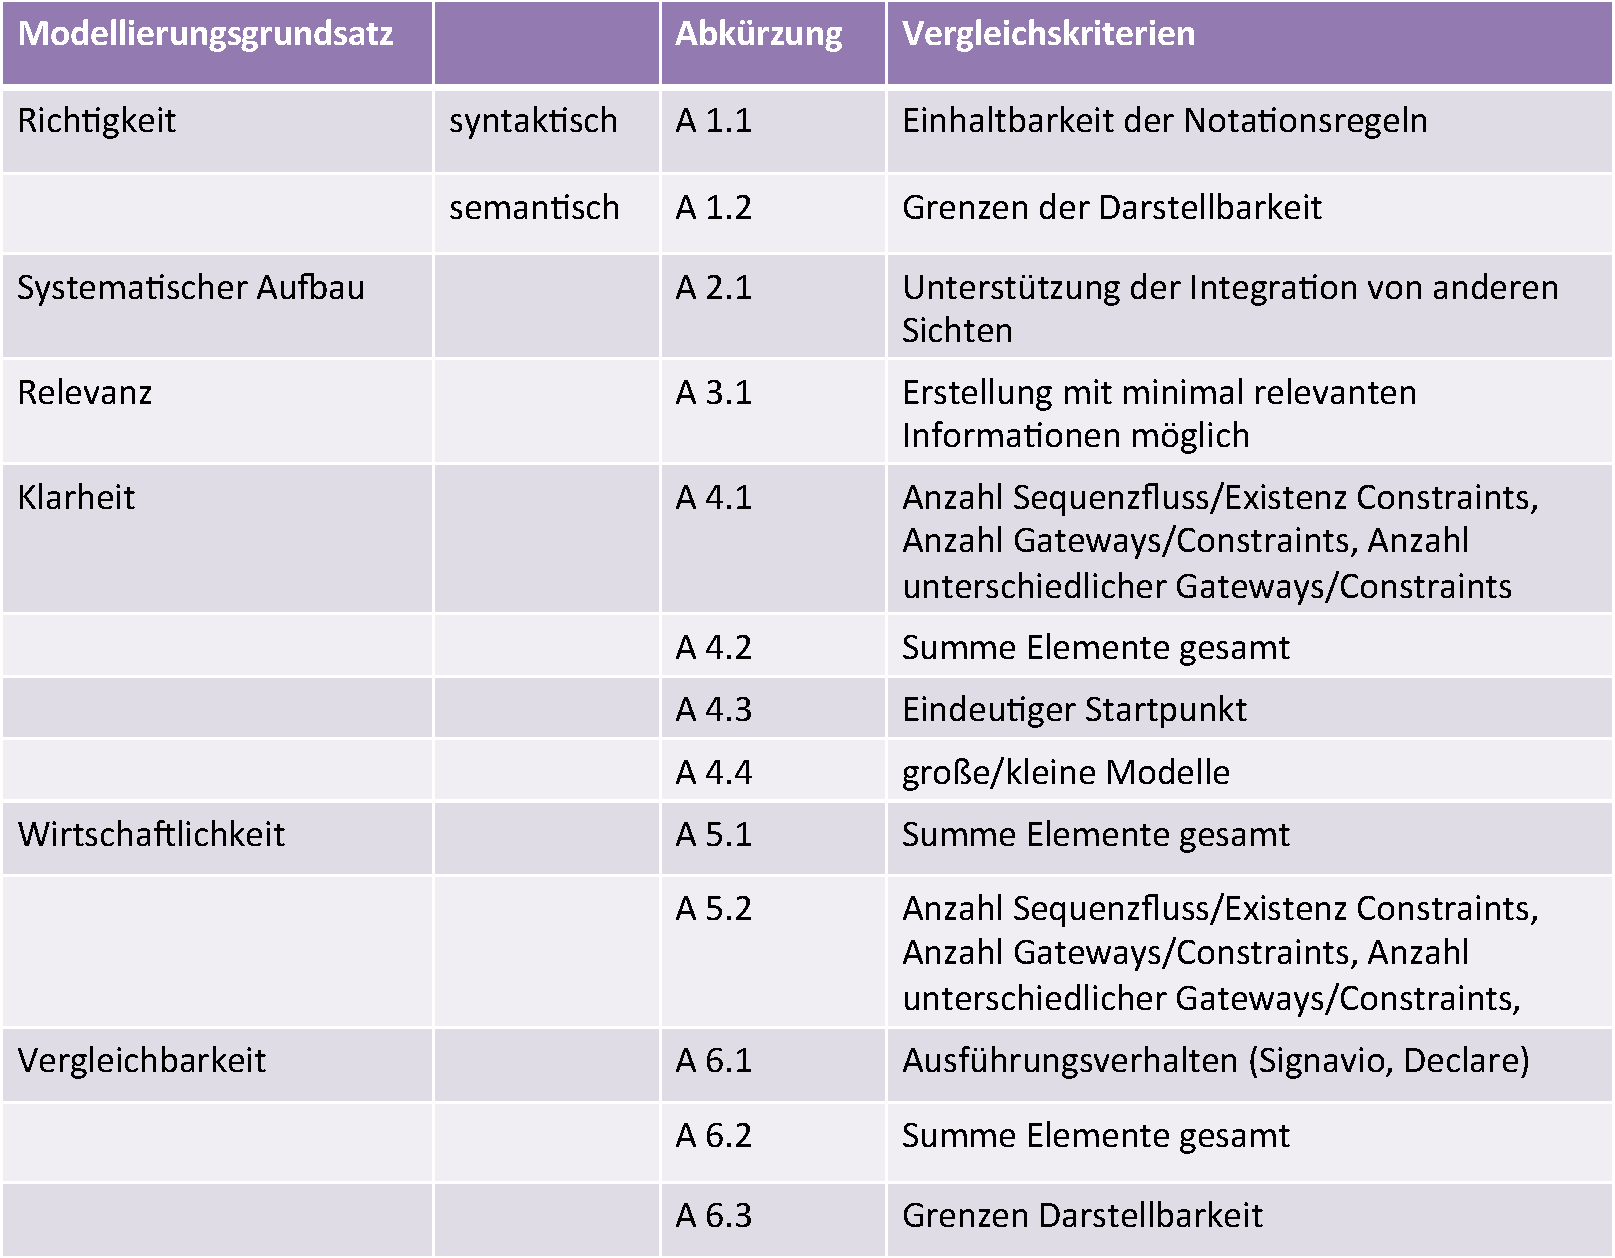
\includegraphics[width=\textwidth]{TabelleKriterien} %pdf, jpg, png...
  \caption{Übersicht Vergleichskriterien}
  \label{fig:TabelleKriterien}
\end{center}
\end{figure}









\chapter{Modellierung für SE-Prozessmodelle}\label{sec:chapter6}
In diesem Kapitel wird ein Vergleich der Anwendbarkeit zwischen imperativer und deklarativer Modellierung für SE-Prozessmodelle gezogen. Als Erstes wird dieser Vergleich in Kapitel 5.1 für das SE-Prozessmodell Scrum durchgeführt. Hierfür wird zunächst in Kapitel 5.1 das der Modellierung zugrunde liegende Modell, das SE-Prozessmodell Scrum, vorgestellt und für die Modellierung analysiert. Danach erfolgt die imperative Modellierung in der imperativen Prozessmodellierungssprache BPMN und anschließend die deklarative Modellierung in der deklarativen Prozessmodellierungssprache ConDec. Danach erfolgt der Vergleich zwischen den beiden Modellen.\newline
Der zweite SE-Prozessmodell, welcher in diesem Kapitel in imperativer und deklarativer Prozessmodellierungssprache verglichen werden soll, ist der Open Unified Process (Open UP). Auch hier erfolgt zunächst eine kurze Einführung in den Open UP in Kapitel 5.2, bevor dieser in Kapitel 5.2.1 analysiert wird, damit er in imperativer, bzw. deklarativer Prozessmodellierungssprache modelliert werden kann. Hiernach erfolgt der Vergleich zwischen den imperativen und deklarativen Prozessmodellen.\newline
Zuletzt werden noch für das V-Modell XT die Prozessmodelle erstellt und verglichen. Eine Einführung in das V-Modell XT erfolgt in Kapitel 5.3. In Kapitel 5.3.1 wird für dieses als Vorbereitung für die Modellierung eine Analyse durchgeführt und es erfolgt die Modellierung in imperativer und deklarativer Prozessmodellierungssprache. Anschließend erfolgt der Vergleich erfolgt hierzu.\newline
Kapitel 5.4 widmet sich dem Vergleich zwischen allen Modellen insgesamt. Hier werden die Ergebnisse der Vergleiche aus den vorigen drei Kapiteln zusammengefasst und es werden allgemeine Schlüsse gezogen.\newline


\section{Scrum}\label{sec:chapter6:Imperative Modellierung}

Der Begriff Scrum stammt aus dem Artikel "The New New Product Development Game", welchen Hirotaka Takeuchi und Ikujiro Nonaka im Harvard Business Review 1986 veröffentlicht haben. Sie beschrieben einen ganzheitlichen Ansatz, bei dem kleine, funktionsübergreifende Teams zusammen an einem gemeinsamen Ziel arbeiten. Dies verglichen sie mit der Scrum-Formation beim Rugby \cite{Pham2012,Takeuchi1986}. \newline
Bei Scrum handelt es sich um ein agiles Prozessmodell, welches seit Anfang 1990 für komplexe Entwicklungen verwendet wird. Agile Prozessmodelle werden den leichtgewichtigen Prozessmodellen zugeordnet \cite{Hanser2010, Lacey2012}. Einen ersten Überblick über das Scrum-Prozessmodell gibt Abbildung \ref{fig:Scrum}.
\begin{figure}[htp]
\begin{center}
  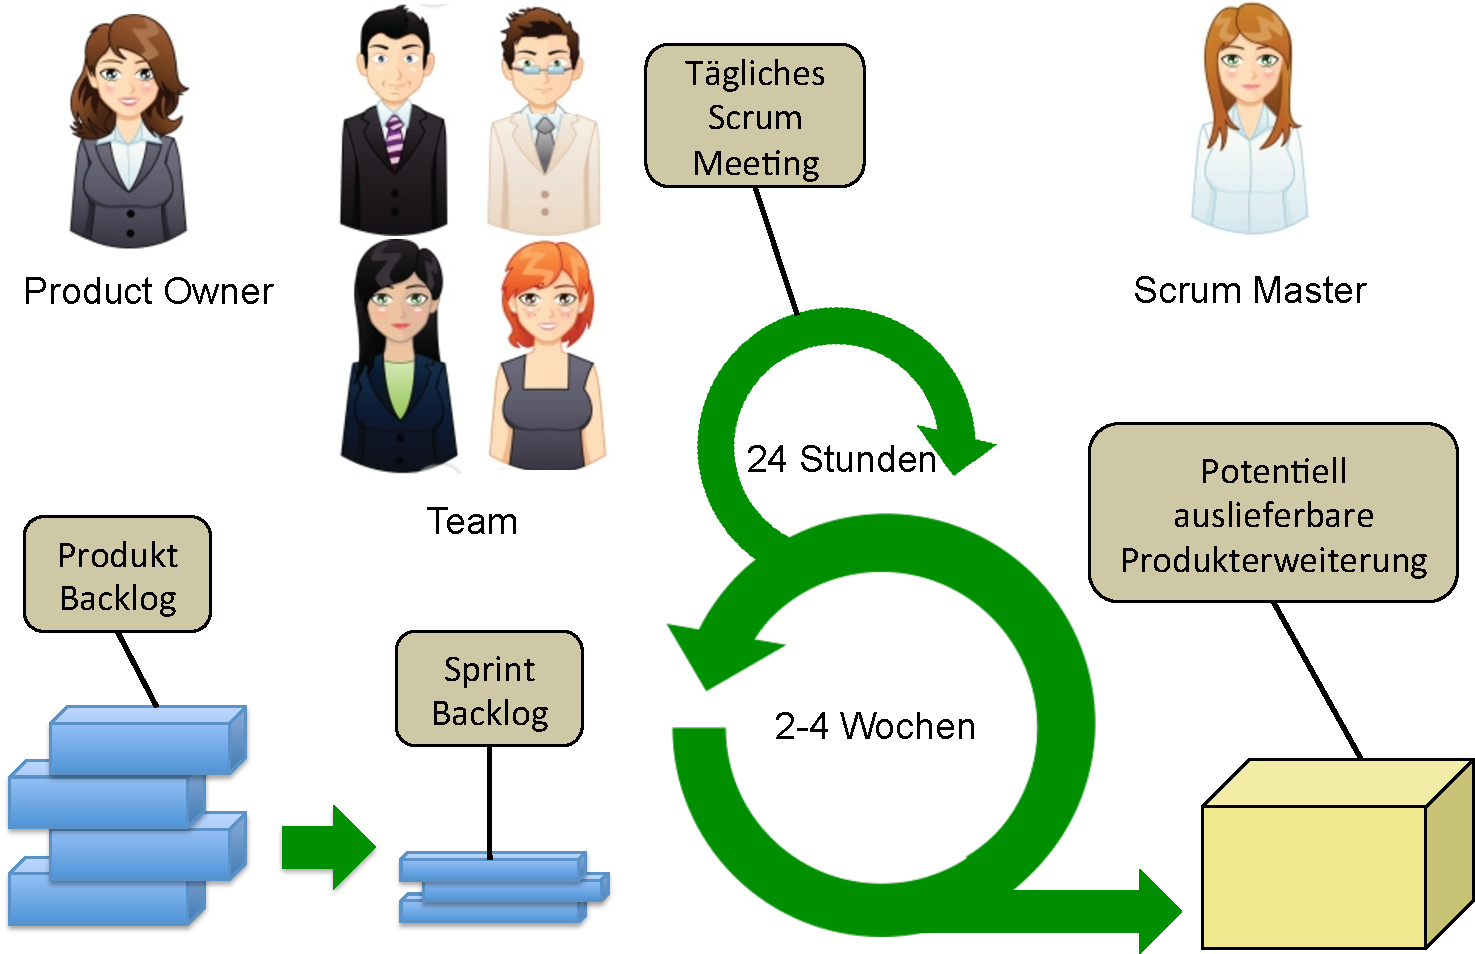
\includegraphics[scale=0.6]{Scrum} %pdf, jpg, png...
  \caption{Scrum Überblick nach \cite{scrum2008}}
  \label{fig:Scrum}
\end{center}
\end{figure}
Der genaue Ablauf im Scrum-Prozessmodell wird nachfolgend analysiert.

\subsection{Analyse Scrum}


Im Scrum-Prozessmodell gibt es nur drei verschiedene Rollen: Den \textit{Product Owner}, das \textit{Team} und den \textit{Scrum Master}. Sämtliche Verantwortlichkeiten innerhalb eines Projektes werden hierbei auf diese drei Rollen aufgeteilt \cite{Schwaber2004}. \newline

Der Procuct Owner ist verantwortlich, die Interessen aller am Projekt beteiligten Personen zu vertreten. Neben der Budgetierung des Projektes erstellt er  Releasepläne und fertigt den \textit{Produkt-Backlog} an, welcher eine Liste mit funktionalen und nicht-funktionalen Anforderungen darstellt \cite{Schwaber2004, Pichler2010,Schwaber2007}. Weiterhin priorisiert er die Aufgaben, welche von den Entwicklern im \textit{Sprint} erledigt werden sollen, so dass die aktuell nützlichsten Elemente die höchste Priorität haben. Er erstellt eine Liste dieser Elemente, welche \textit{Sprint-Backlog} genannt wird \cite{Henning2011, Schwaber2007,Pichler2010}. Der Procuct Owner ist ebenfalls zuständig für das Annehmen, bzw. Ablehnen der Arbeitsergebnisse \cite{eclipseScrum}. \newline

Die Teams bestehen bei Scrum für gewöhnlich aus fünf bis neun Mitgliedern und verwalten sich selbst. Ihre Tätigkeiten müssen erfolgreich sein, liegen aber in ihrer eigenen Verantwortung \cite{Pries2011, Wolf2011}. Alle Teammitglieder sind gemeinsam für den Erfolg eines jeden \textit{Sprints} und des gesamten Projektes zuständig \cite{Pichler2010}. \newline

Der Scrum-Master ist für den gesamten Scrum-Prozess verantwortlich. Dies schließt die Vermittlung von Scrum-Inhalten (z.B. Schulungen) und die Implementation von Scrum in die Unternehmenskultur ein \cite{Pichler2010}. Er überwacht die Sprint- Tasks, um sicher zu gehen, dass der Sprint erfolgreich verläuft.\newline

Bei Scrum wird die Entwicklung in mehrere kurze Zyklen, also Iterationen eingeteilt. Eine einzelne Iteration wird bei Scrum \textit{Sprint} genannt \cite{Henning2011}. Die Dauer eines Sprints beträgt zwei bis vier Wochen. Am Ende eines jeden Sprints muss das Team ein lauffähiges Produkt abliefern \cite{Wolf2011}. Vor jedem Sprint findet ein \textit{Sprint Planning Meeting} statt, welches sich aus zwei Teilen zusammensetzt \cite{Pichler2010}. Im ersten Teil findet eine Planung des nächsten Sprints statt \cite{Lacey2012}. Hierfür präsentiert der Product Owner dem Team eine Liste der Product-Backlog-Elemente mit der aktuell höchsten Priorität \cite{Schwaber2004, Schwaber2007,Pichler2010}. Diese Liste wird \textit{Sprint-Backlog} genannt \cite{Wolf2011}. Das Team hat die Möglichkeit, Fragen bezüglich Inhalt, Zweck, Bedeutung und Absichten der Sprint-Backlog-Elemente zu stellen. Anschließend werden die einzelnen Elemente aus dem Sprint-Backlog in sogenannte \textit{Tasks} aufgeteilt, welche jeweils eine ideale Bearbeitungszeit von zwei bis vier Stunden haben, aber niemals länger als zwei Tage dauern sollten \cite{Wolf2011}. Das Team kann sich die Aufgaben eigenverantwortlich aufteilen und muss sich anschließend dem Product  Owner verpflichten, die Tasks bis zum Abschluss des Sprints zu erledigen \cite{Wolf2011, Keith2010,Pichler2010}.
Das Team trifft sich während des Sprints täglich in einem 15-minütigen Meeting, dem \textit{täglichem Scrum-Meeting}. Dabei redet das Team über seinen Fortschritt und eventuelle Probleme bei seiner Arbeit \cite{Keith2010}. Hier muss jedes Teammitglied die nachfolgenden drei Fragen beantworten \cite{Wolf2011}:
   \begin{enumerate}
      \item Was habe ich seit gestern erreicht?
      \item Was werde ich heute erreichen?
      \item Was blockiert mich?
      \end {enumerate}
      
\subsection{Imperative Modellierung Scrum}

Abbildung \ref{fig:ScrumImperativ} zeigt die imperative Modellierung von Scrum. Im Prozess gibt es die drei verschiedenen Rollen \textit{Product Owner}, \textit{Team} und \textit{Scrum Master}, was im Prozessmodell durch drei verschiedene Swimlanes dargestellt ist. Manche Aktivitäten werden auch von mehreren Rollen ausgeführt. Da dies jedoch in BPMN nicht darstellbar ist, werden die entsprechenden Aktivitäten nachfolgend immer dem Hauptakteur zugeteilt.\newline
Parallel zu allen anderen Aktivitäten des Teams und des Product Owners muss der Scrum-Master stets den Scrum-Prozess managen. Dies wird im Prozessmodell durch das parallele Gateway dargestellt. \newline
Der Product Owner schätzt als erste Aktivität den Product Backlog ab. Anschließend priorisiert er den Product Backlog und erstellt parallel dazu die Releasepläne. \newline
Wenn alle zwei bis vier Wochen ein neuer Sprint beginnt, was hier durch ein Zeitereignis dargestellt ist, so wird zuerst das Sprint Planning Meeting durchgeführt. Dies ist hier als Unterprozess in Abbildung \ref{fig:ScrumImperativUnter} dargestellt. Zunächst priorisiert der Product Owner die Anforderungen, welche während des Sprints erledigt werden müssen, und erstellt danach den Sprint Backlog. Anschließend teilt sich das Team selbstständig die Sprint Backlog-Elemente in Tasks ein.\newline
Im Anschluss findet ein Sprint-Rückblick statt (Abbildung \ref{fig:ScrumImperativ}) und der Product Owner veranstaltet ein Sprint Review Meeting.\newline
Das Team führt während des Sprints täglich ein 15-minütiges Scrum Meeting durch und jedes Teammitglied arbeitet eine Task nach der anderen ab. Dies wird hier als Schleife dargestellt: Solange noch weitere Tasks vorhanden sind, führt das Exklusive Gateway immer wieder zurück zur Aktivität \textit{Tasks abarbeiten}. Erst wenn keine weiteren Tasks mehr vorhanden sind, führt der Prozess weiter zum nächsten Entscheidungspunkt.\newline
Sind noch weitere Aufgaben im Product Backlog vorhanden, die noch erledigt werden müssen, so beginnt ein weiterer Sprint, was hier durch eine Rückschleife dargestellt ist. Ist jedoch schon der komplette Product Backlog abgearbeitet, so endet der Prozess hier.


\begin{sidewaysfigure}[htp]
\begin{center}
  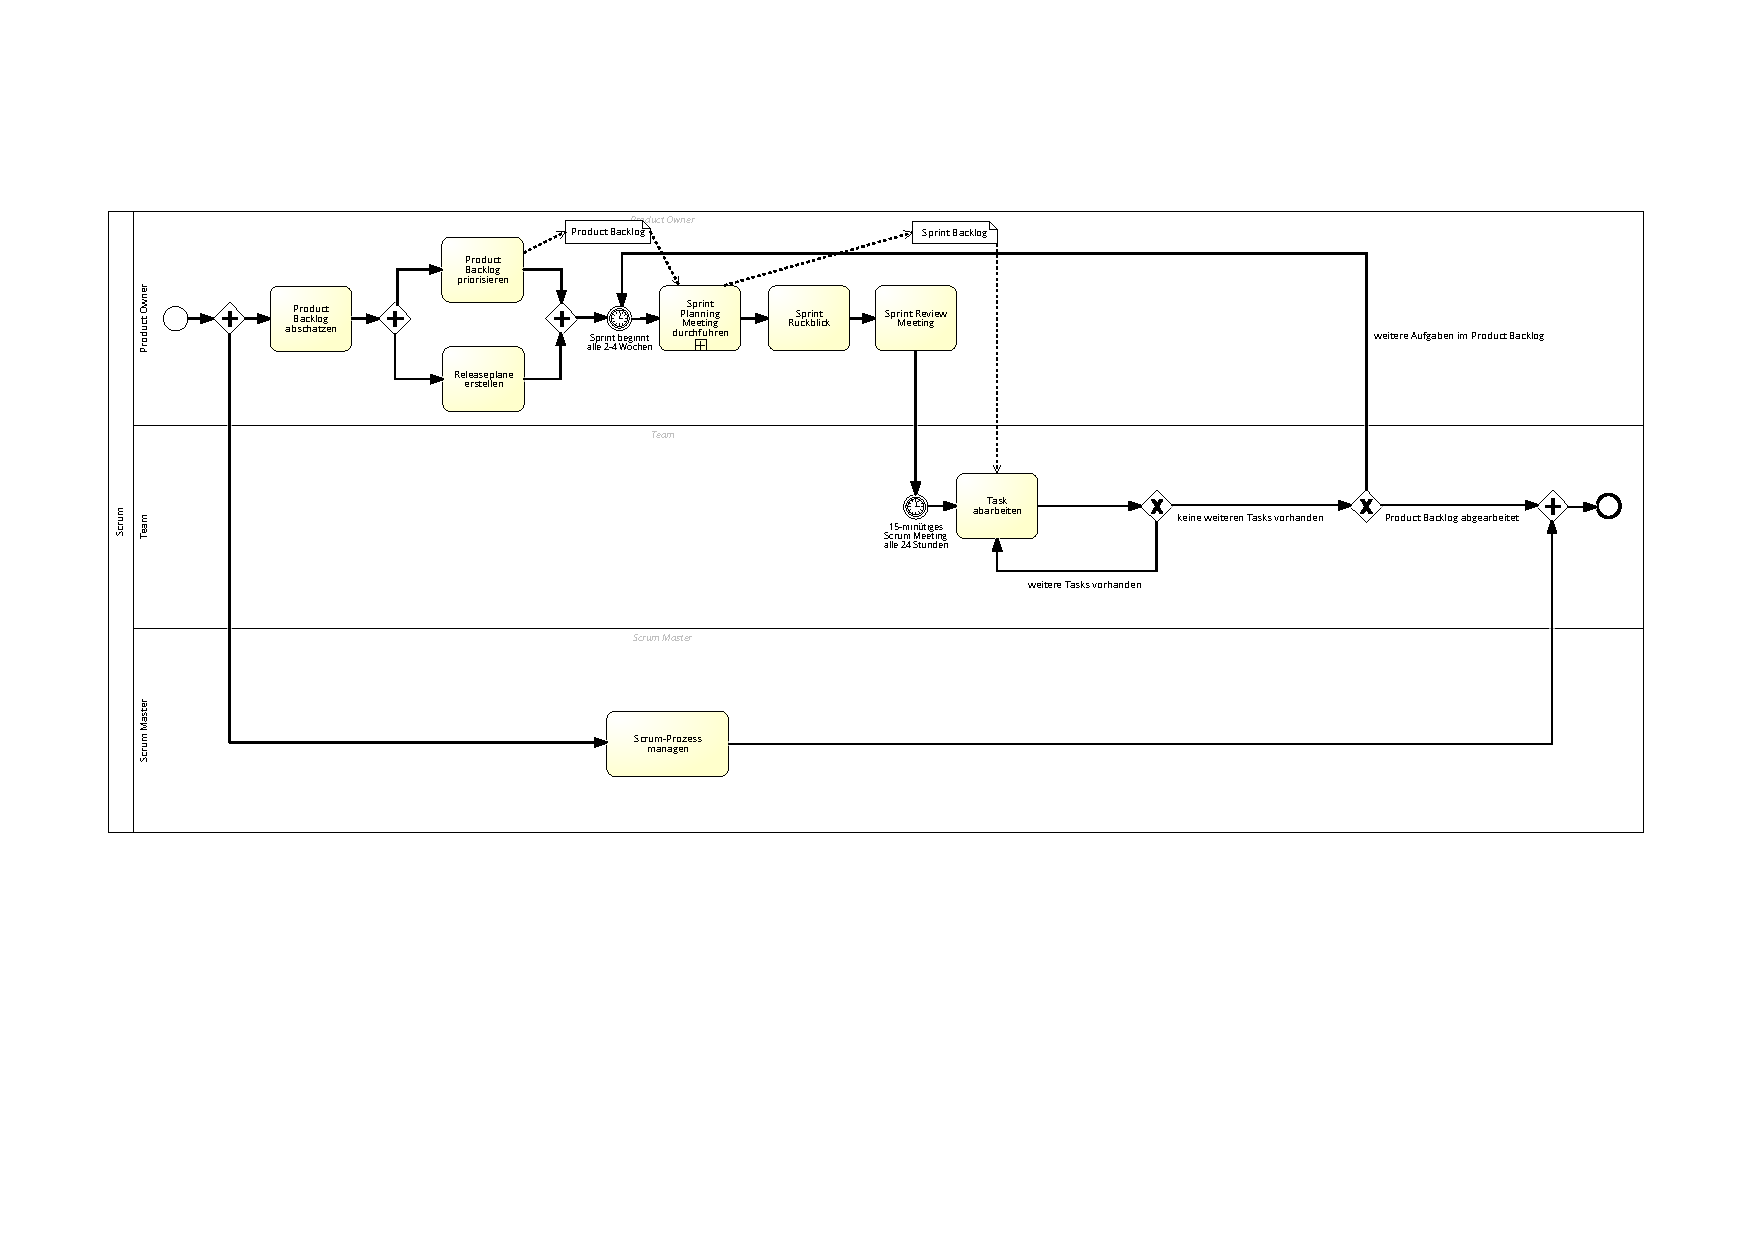
\includegraphics[width=\textwidth]{ScrumImperativ} %pdf, jpg, png...
  \caption{Imperative Modellierung Scrum}
  \label{fig:ScrumImperativ}
\end{center}
\end{sidewaysfigure}

\begin{figure}[htp]
\begin{center}
  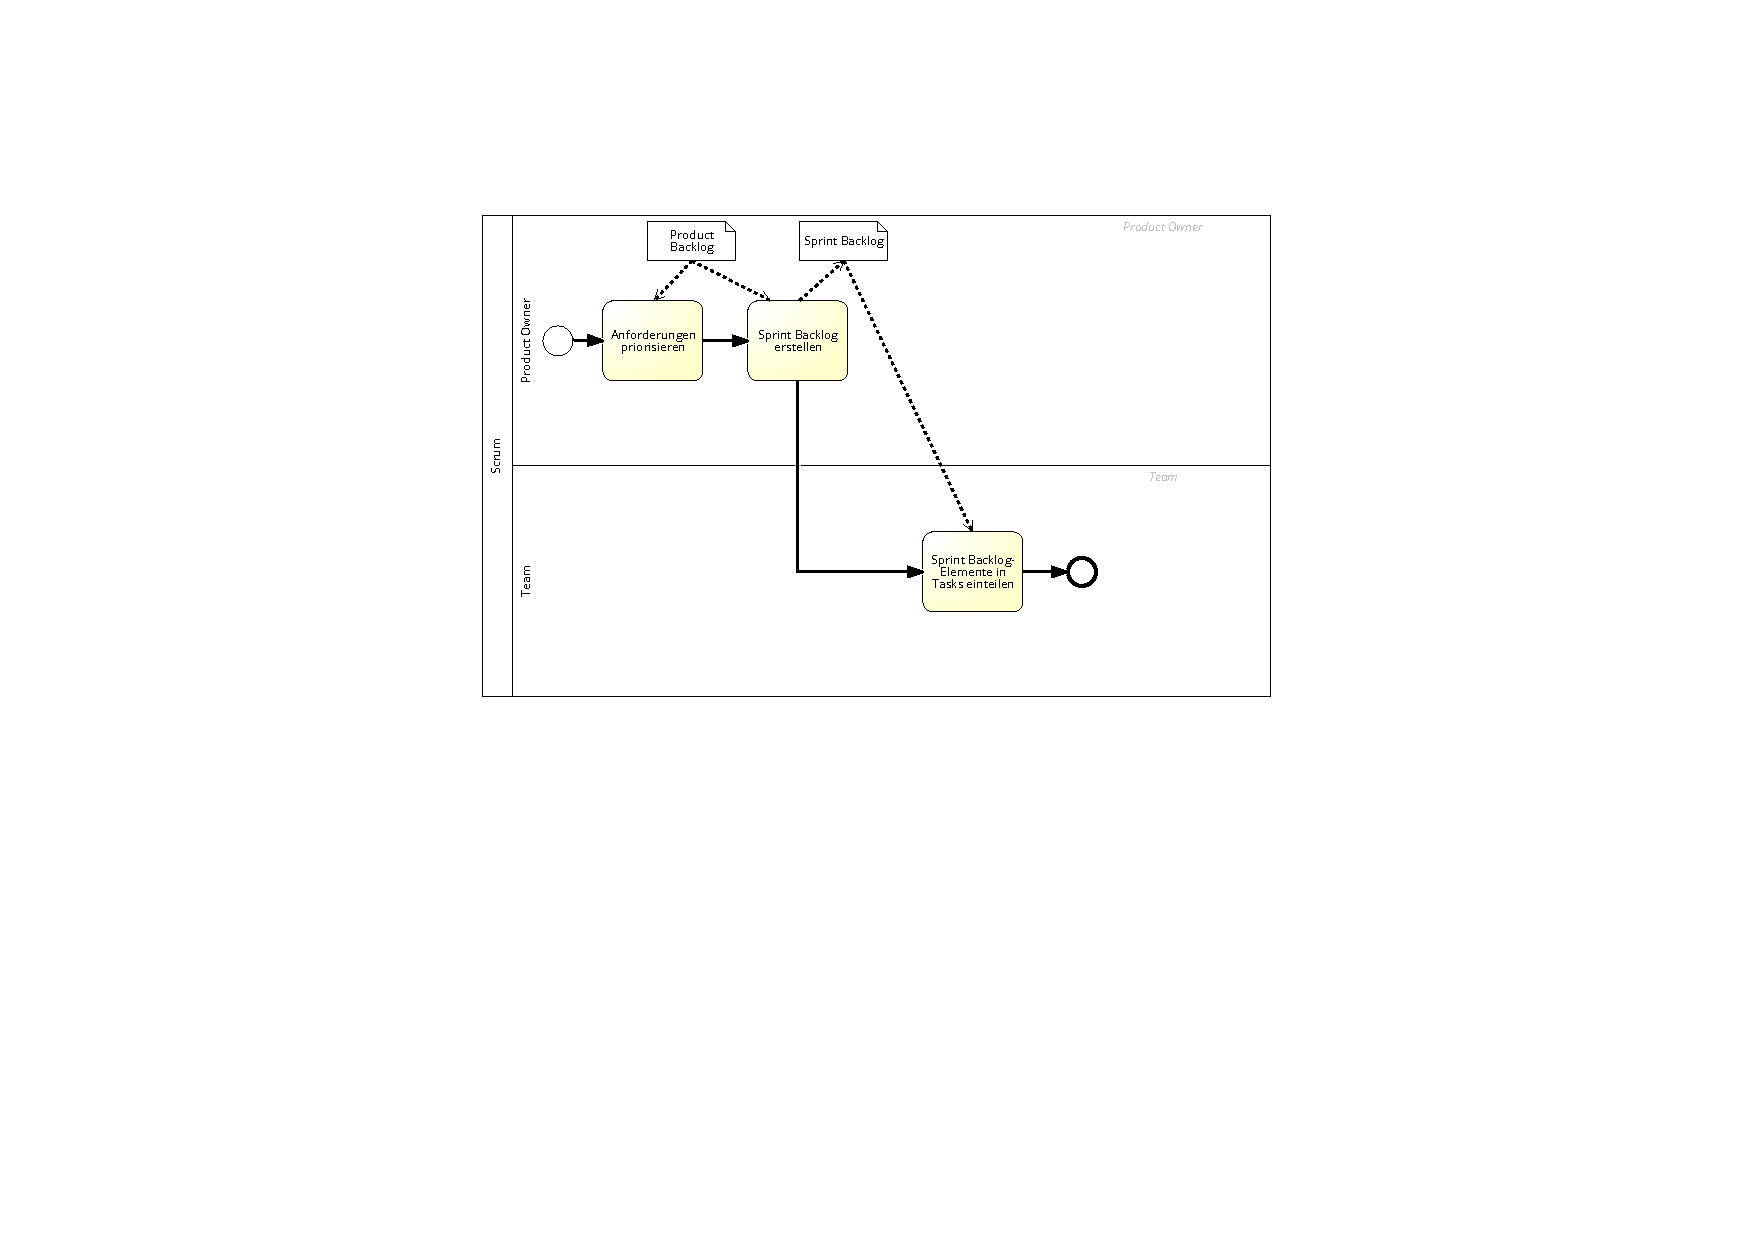
\includegraphics[scale=0.7]{ScrumImperativUnter} %pdf, jpg, png...
  \caption{Imperative Modellierung Scrum Unterprozess}
  \label{fig:ScrumImperativUnter}
\end{center}
\end{figure}
\clearpage

\subsection{Deklarative Modellierung Scrum}

Abbildung \ref{fig:ScrumDecHaupt} zeigt die deklarative Modelliereung von Scrum. Der Prozess beginnt mit der Aktivität "Product Backlog abschätzen". Dies ist hier durch das Init-Constraint gekennzeichnet. Weiterhin wird diese Aktivität im Prozess genau einmal ausgeführt was durch das Exactly (1)- Constraint dargestellt ist. Das Constraint \textit{succession} gibt an, dass die Aktivität \grqq Product Backlog abschätzen\grqq \ vor den Aktivitäten \grqq Product Backlog priorisieren\grqq \ und \grqq Releasepläne erstellen\grqq \ ausgeführt werden müssen und dass die Aktivitäten \grqq Product Backlog priorisieren\grqq \ und \grqq Releasepläne erstellen\grqq \ auf jeden Fall nach \grqq Product Backlog abschätzen\grqq \ durchgeführt werden müssen. \grqq Product Backlog priorisieren\grqq \ und \grqq Releasepläne erstellen\grqq \ werden ebenfalls genau einmal ausgeführt, was durch das Exactly (1)- Constraint festgelegt wird.  \newline

Nach deren Ausführung muss die Aktivität \textit{alle 2-4 Wochen Sprint Planning Meeting durchfuehren} erfolgen. Der zugehörige Unterprozess ist in Abbildung \ref{fig:ScrumDecUnterprozess} zu finden. Hier sind die Aktivitäten \grqq Anforderungen priorisieren\grqq, \grqq Sprint Backlog erstellen\grqq \ und \grqq Sprint-Backlog-Elemente in Tasks einteilen\grqq \ durch das Constraint \textit{precedence} miteinander verbunden, um die Einhaltung deren Reihenfolge nacheinander zu gewährleisten. Außerdem dürfen diese Aktivitäten pro Ausführung des Unterprozesses, also pro Prozessinstanz nur einmal ausgeführt werden.\newline
Nach der Ausführung der Aktivitäten des Unterprozesses Sprint-Planning-Meeting durchführen, muss im Anschluß die Aktivität \grqq Sprint Rückblick\grqq \ durchgeführt werden. Dies wird durch das Constraint \textit{chain response} sichergestellt.Eine erneute Ausführung von \grqq alle 24 Stunden 15-minütiges Scrum-Meeting durchführen\grqq \ ist erst nach Durchführung von \grqq Sprint Rückblick\grqq \ möglich (Constraint \textit{alternate precedence}). Hierdurch wird eine Schleife modelliert, welche den immer wiederkehrenden Sprint simuliert.\newline
Die Aktivitäten \grqq alle 24 Stunden 15-minütiges Scrum-Meeting durchführen\grqq \ und \grqq Tasks abarbeiten\grqq \ können während des Sprints so oft wie nötig durchgeführt werden. Die Aktivitäten \grqq alle 24 Stunden 15-minütiges Scrum-Meeting durchführen\grqq \ und \grqq Tasks abarbeiten\grqq \ müssen jedoch nebeneinander ausgeführt werden, was durch das Constraint \textit{succession} beschrieben ist. \newline


\begin{figure}[htp]
\begin{center}
  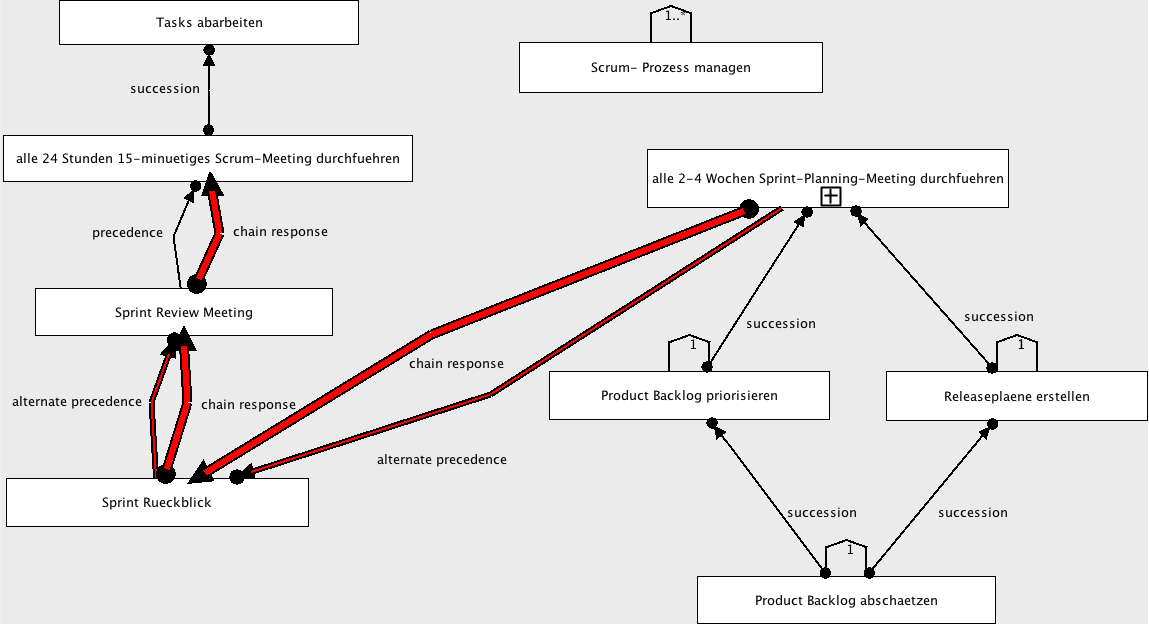
\includegraphics[width=\textwidth]{ScrumDecHaupt} %pdf, jpg, png...
  \caption{Deklarative Modellierung Scrum}
  \label{fig:ScrumDecHaupt}
\end{center}
\end{figure}



\begin{figure}[htp]
\begin{center}
  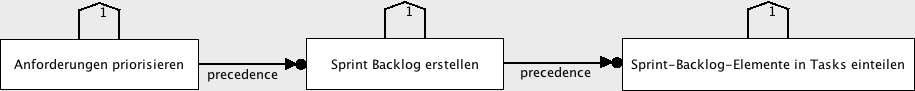
\includegraphics[width=\textwidth]{ScrumDecUnterprozess} %pdf, jpg, png...
  \caption{Deklarative Modellierung Scrum-Unterprozess Sprint-Planning-Meeting durchführen}
  \label{fig:ScrumDecUnterprozess}
\end{center}
\end{figure}
\clearpage

\subsection{Vergleich}

Der Vergleich zwischen den in der deklarativen Prozessmodellierungssprache ConDec und in der imperativen Prozessmodellierungssprache BPMN erstellten Scrum Prozessmodell wird im Folgenden anhand der in Kapitel 4 definierten Anforderungen durchgeführt. Auf Grund der dort definierten Vergleichskriterien wurden nachfolgend die Aktivitäten, die Anzahl der Constraints/Gateways, Anzahl der Sequenzflusselemente/Existenz, Anzahl unterschiedlicher Gateways/Constraints sowie die Summe der Elemente insgesamt in beiden Modellen gezählt. Hierdurch können im Folgenden die Modelle anhand der Vergleichskriterien miteinander verglichen werden. \newline
Wie Abbildung \ref{fig:ScrumExcel} entnommen werden kann, unterscheidet sich die Anzahl der Aktivitäten zwischen den in BPMN und ConDec modellierten Prozessmodellen nicht voneinander. In jedem Prozessmodell gibt es 12 Aktivitäten.\newline

\begin{figure}[htp]
\begin{center}
  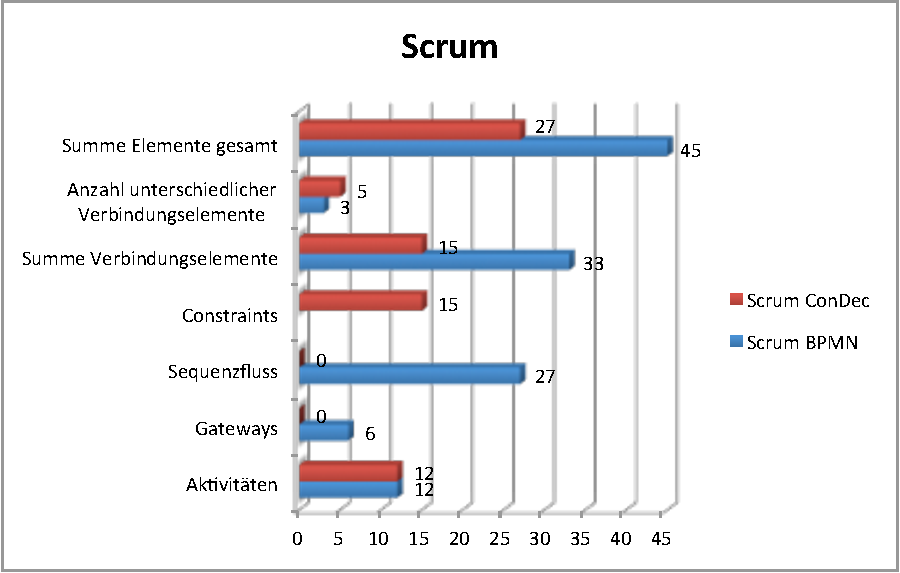
\includegraphics[scale=0.8]{ScrumExcel} %pdf, jpg, png...
  \caption{Vergleich der Anzahl der Elemente Scrum}
  \label{fig:ScrumExcel}
\end{center}
\end{figure}


Zudem braucht es in BPMN sechs Gateways und 26 Sequenzflusselemente, um den Ablauf des Metamodells darzustellen. Bei Verwendung von ConDec werden 13 Constraints (vier unterschiedliche) und sieben Existenz Constraints zur Darstellung der Abfolge der Aktivitäten benötigt. In BPMN werden sechs Gateways (zwei unterschiedliche) verwendet.\newline


Die syntaktische \textit{Richtigkeit} [A 1.1] kann bei beiden Modellierungssprachen eingehalten werden, da bei beiden Prozessmodellierungssprachen die Notationsregeln zur korrekten Darstellung des Prozessablaufes eingehalten werden können. Dies hat das Testen der beiden Modelle in Signavio, bzw. Declare bestätigt.\newline
Die semantische \textit{Richtigkeit} [A 1.2] lässt sich mit BPMN in Bezug auf Rollen und Artefakte besser einhalten, als mit ConDec. Da es bei ConDec keine Möglichkeit gibt, Rollen und Artefakte im Prozessmodell zu visualisieren fehlen diese Informationen. Die Rollen und Artefakte können zwar in Declare abgebildet werden, jedoch gibt es in ConDec hierfür keine Notationselemente, um Rollen und Artefakte im Prozessmodell selbst sichtbar zu machen. Aus diesem Grund müssen diese Informationen beim Modellieren weggelassen werden, was zur Folge hat, dass das im Metamodell beschriebene Verhalten nicht vollständig abgebildet werden kann und somit leidet auch der Nutzen des Modells.\newline
In Anbetracht der syntaktischen Richtigkeit sind BPMN und ConDec gleich gut zur Modellierung geeignet. Bei Betrachtung der semantischen Richtigkeit ist somit BPMN die geeignetere Modellierungssprache.


Nur BPMN bietet die Möglichkeit, Artefakte im Prozessmodell zu visualisieren und lässt somit die Integration anderer Sichten in das Modell zu. Somit kann der Modellierungsgrundsatz des \textit{systematischen Aufbaus} [A 2.1] nur von BPMN eingehalten werden. Da ConDec dies nicht zulässt, schmälert es die Eignung von ConDec zum Modellieren in Bezug auf Softwareprozessmodelle. Hierdurch können wichtige Informationen aus dem Metamodell nicht abgebildet werden. \newline 

Lediglich die mit BPMN erstellten Prozessmodelle können mit minimal relevanten Informationen erstellt werden. Der Grund dafür ist wiederum die fehlende Visualisierungsmöglichkeit von Rollen und Artefakten. Somit kann die \textit{Relevanz} [A 3.1] nur von BPMN eingehalten werden.\newline

Bei Untersuchung der \textit{Klarheit} lässt sich feststellen, dass sich die Anzahl der Sequenzflusselemente/Existenz Constraints zwischen BPMN (26) und ConDec (7) unterscheidet. Ebenfalls gibt es eine Differenz bei der Anzahl der Gateways (6)/Constraints (13) und der Anzahl der unterschiedlichen Gateways (2)/Constraints (4) zwischen BPMN und ConDec.\newline

Wie in Kapitel 4 bereits erwähnt [A 4.1], kann sich eine größere Anzahl an Gateways/Constraints negativ auf die Verständlichkeit auswirken. Hier ist die Anzahl bei ConDec mehr als doppelt so hoch wie bei BPMN. In BPMN werden insgesamt zwei verschiedene Gateways (ein exklusives Gateway und ein paralleles Gateway) verwendet zur Darstellung von Verzweigungen. In ConDec werden vier verschiedene Constraints zur Darstellung genutzt. Zudem existiert im ConDec Modell keine eindeutige Start Aktivität [A 4.2], welche durch das Init-Constraint markiert ist. Dies liegt daran, dass mehrere Aktivitäten als Einstiegsaktivität in Frage kommen. Die möglichen Einstiegsaktivitäten sind jedoch nicht auf den ersten Blick ersichtlich. Dies steigert die Komplexität des ConDec Modelles. \newline
 Das BPMN-Modell weißt nur im Hinblick auf die Anzahl von Sequenzflusselementen im Gegensatz zu Existenz Constraints einen höheren Wert auf. Wie in Kapitel 4 festgelegt wird die Anzahl Sequenzfluss/Existenz Constraints [A 4.1] einfach gewichtet und die Anzahl Gateways/Constraints und Anzahl unterschiedlicher Gateways/Constraints beim ConDec Modell doppelt [A 4.1] gewichtet. Somit weist das mit ConDec erstellte Modell in zwei jeweils doppelt gewichteten Punkten eine höhere Komplexität auf und das BPMN Modell nur in einem einfach gewichteten Punkt. Da noch die fehlende Startmarkierung bei ConDec [A 4.2] hinzu kommt, wird das mit ConDec erstellte Modell auf Grund der definierten Anforderungen in Kapitel 4 als komplexer eingestuft.
\newline
Somit ist hier BPMN in Bezug auf die \textit{Klarheit} geeigneter zum Modellieren als ConDec, da es die beiden unterkriterien [A 4.1] und [A 4.2] besser erfüllt.\newline

Die \textit{Wirtschaftlichkeit} unterscheidet sich bei den beiden Modellierungssprachen. Das mit BPMN erstellte Modell weist 26 Sequenzflusselemente auf und das mit ConDec erstellte Modell sieben Existenz Constraints. Bei ConDec hingegen werden mehr Constraints (13, 4 verschiedene) benötigt als Gateways (6, 2 verschiedene) bei BPMN. Hier gilt für das Kriterium [5.1] die gleiche Argumentation wie bei \textit{Klarheit, [4.1]}. Da die Anzahl Sequenzfluss/Existenz Constraints [A 5.1] einfach gewichtet und die Anzahl Gateways/Constraints und Anzahl unterschiedlicher Gateways/Constraints beim ConDec Modell doppelt [A 5.1] gewichtet wird, weist das ConDec Modell eine öhere komplexität auf und der Modellierer hat somit einen höheren Aufwand beim erstellen.\newline
Aus diesem Grund erfüllt BPMN bei diesem Modell die \textit{Wirtschaflichkeit} besser als ConDec.\newline

Die \textit{Vergleichbarkeit} in Betracht des Ausführungsverhaltens der beiden Modelle wurde durch Testausführungen in den Modellierungstools Signavio und Declare gewährleistet [A 6.1].\newline
Bei BPMN weist das erstellte Modell insgesamt mehr Elemente auf. Während bei ConDec insgesamt 32 Elemente benötigt werden, werden zur Darstellung des gleichen Sachverhaltes bei BPMN 44 Elemente verwendet [A 6.2]. \newline
Bei ConDec müssen Informationen wie Rollen und Artefakte weggelassen werden, während sie in BPMN dargestellt werden können [A 6.3].\newline
Die \textit{Vergleichbarkeit} kann zwar in Bezug auf das Ausführungsverhalten von beiden Sprachen eingehalten werden [A 6.1]. BPMN weist jedoch insgesamt mehr Elemente auf [A 6.2] und ConDec kann die \textit{Vergleichbarkeit} in Bezug auf die Darstellbarkeit von Rollen und Artefakten nicht einhalten [A 6.3]. Somit kann ein Kriterium [6.2] von ConDec besser eines [A 6.3] von BPMN eingehalten werden. Das kriterium [6.1] kann von beiden eingehalten werden. Somit liegt hier keine der beiden Prozessmodellierungssprachen vorne.\newline

Abbildung \ref{fig:TabelleScrum} zeigt die Ergbenisse des Vergleichs von BPMN und ConDec nochmals in der Zusammenfassung. Somit liegt BPMN bei den Grundsätzen \textit{Richtigkeit}, \textit{systematischer Aufbau}, \textit{Klarheit} und \textit{Vergleichbarkeit} vorne, bei den Grundsätzen \textit{Wirtschaftlichkeit} und \textit{Relevanz} liegen BPMN und ConDec gleich auf. \newline

\begin{figure}[htp]
\begin{center}
  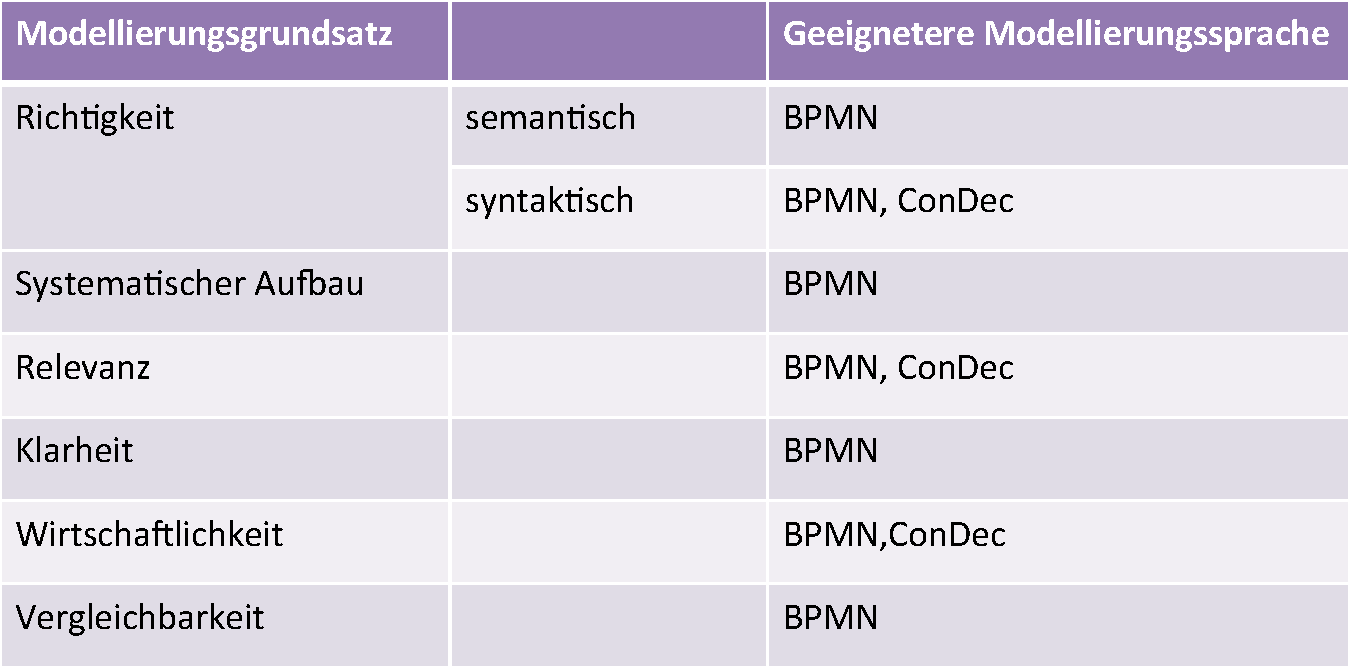
\includegraphics[scale=0.6]{TabelleScrum} %pdf, jpg, png...
  \caption{Zusammenfassung Vergleich Scrum}
  \label{fig:TabelleScrum}
\end{center}
\end{figure}




\section{Open Unified Process (Open UP)}


Der Open Unified Process, kurz Open UP ist eine frei zugängliche Variante des Rational Unified Process, welcher ein sehr bekannter Entwicklungsprozess ist \cite{hauber2010}.  Er ist Teil des Eclipse Process Frameworks. Open UP ist ein iterativer, inkrementeller und minimaler Prozess, aber dennoch vollständig und erweiterbar \cite{Gau2006, Basem2010}. Der Prozess ist minimal gehalten, weil er nur die wesentlichen Inhalte einbezieht. Er ist außerdem auch erweiterbar, da er als Grundlage herangezogen werden kann und mit weiteren Prozessfragmenten aufgestockt und nach Belieben zugeschnitten werden kann \cite{Wang2007}. Das Konzept des Open UP ist, den Prozess zu vergrößern, sich aber auf das Minimum, welches für das Projekt benötigt wird, zu beschränken, anstatt zu versuchen große, überladene Prozesse zu verstehen und diese dann zu verkleinern \cite{ambler2012}.  \newline



Open UP ist auf kleine Teams ausgerichtet, bei denen bei der Zusammenarbeit räumliche Nähe besteht. Die Teammitglieder haben hierbei die Freiheit, ihre eigenen Entscheidungen bezüglich ihren aktuellen Aufgaben und Prioritäten zu treffen, um die Anforderungen der Stakeholder zu erfüllen. Das Team trifft sich täglich, um über den aktuellen Status zu reden \cite{OpenUPProcess}.\newline
Es werden Rollen, Aufgaben, Artefakte und Ebenen in Open UP definiert. Dies soll ermöglichen, dass verschiedene Sichten, die sich in ihrem Detaillierungsgrad unterscheiden, auf das Projekt möglich sind \cite{freudenreichevaluierung}. Einen ersten Überblick über Open UP gibt Abbildung \ref{fig:openup}.


\begin{figure}[htp]
\begin{center}
  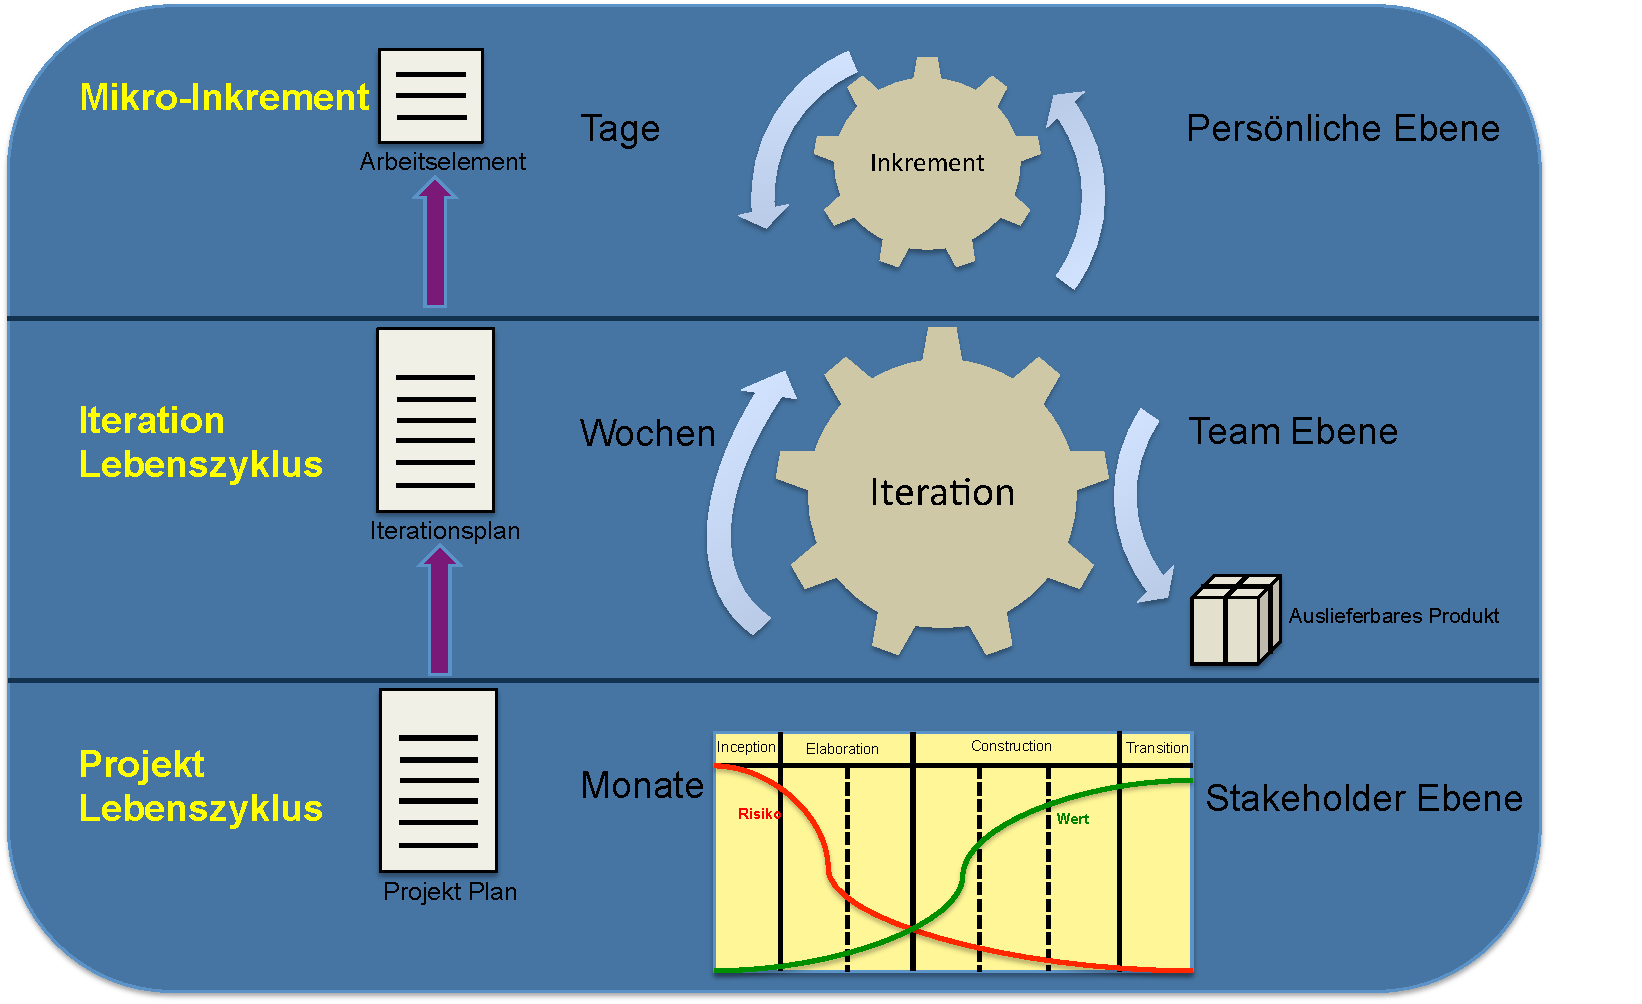
\includegraphics[width=\linewidth]{openup} %pdf, jpg, png...
  \caption{Open UP Überblick nach \cite{eclipseopenup}}
  \label{fig:openup}
\end{center}
\end{figure}

Der Open UP wird im Folgenden analysiert.

\subsection{Analyse Open UP}


Auf der persönlichen Ebene teilen sich die Teammitglieder ihre Arbeit in \textit{Mikro-Inkremente} ein. Diese stellen das Ergebnis von Stunden, bzw. wenigen Tagen Arbeit dar. Die Arbeit entwickelt sich somit ein Mikro-Inkrement weiter und der Fortschritt kann Tag für Tag nachvollzogen werden. Die Teammitglieder teilen ihre Fortschritte täglich miteinander, was die Arbeitstransparenz und das Vertrauen erhöht und die Teamarbeit fördert \cite{eclipseopenup}. \newline

Auf der Team-Ebene wird das Projekt in Iterationen unterteilt, welche einen Zeitraum von mehreren Wochen umfassen. Das Ziel ist es, am Ende eines Iterationszyklus ein funktionierendes Softwareinkrement zu haben. Dieses Inkrement stellt eine Version des Softwaresystems dar welche zusätzliche oder verbesserte Funktionalitäten besitzt als die vorherige Version \cite{Basem2010}.  In jeder Iteration wird ein Iterationsplan angefertigt,  der vorgibt, was in dieser Iteration geliefert werden muss und auf welchen sich das Team verpflichten muss \cite{freudenreichevaluierung}.

Auf Stakeholder-Ebene wird diesen durch den \textit{Projektlebenszyklus} die Möglichkeit gegeben, die Projektfinanzierung, den Umfang, das Risiko und andere Aspekte des Prozesses zu kontrollieren.
Der Open UP teilt den \textit{Projektlebenszyklus} in die vier Phasen \textit{Inception}, \textit{Elaboration}, \textit{Construction} und \textit{Transition} ein, über welche Abbildung \ref{fig:Phasen} einen Überblick gibt \cite{eclipseopenup}.

\begin{figure}[htp]
\begin{center}
  \includegraphics[width=\linewidth]{Lebenszyklusopenup} %pdf, jpg, png...
  \caption{Phasen Open UP nach \cite{eclipseopenup}}
  \label{fig:Phasen}
\end{center}
\end{figure}


In jeder Phase finden eine oder mehrere Iterationen statt und werden mit einem Meilenstein abgeschlossen \cite{Basem2010}. In der Phase Inception ist dies der Zielsetzungmeilenstein, in der Phase Elaboration der Architekturmeilenstein, in der Phase Construction der Einsatzfähigkeitmeilenstein und in der Phase Transition der Produktreleasemeilenstein. Tabelle \ref{tab:tab1} zeigt die Abläufe den Iterationen in den einzelnen Phasen und die zugehörigen Zielstellungen.
\begin{longtable}{|p{7cm}|p{8cm}|}
\hline
Vorlagenmodell Iterationen & Zielsetzung der Phase \\
\hline
Inception Phase Iteration 
\begin {itemize}
\item Iteration starten 
 \item  Iteration planen und verwalten
 \item  Anforderungen festlegen und verfeinern 
  \end{itemize}
   &
  
  \begin {itemize}
\item Verstehen, was zu bauen ist
 \item Die wichtigsten Systemfunktionen verstehen 
\item Mindestens eine mögliche Lösung bestimmen
\item Kosten, Zeitplan und Risiken verstehen, welche mit dem Projekt verbunden sind
  \end{itemize}

 \\
\hline
 Elaboration Phase Iteration 
   \begin {itemize}
   \item Iteration planen und verwalten
   \item Anforderungen erheben und verfeinern
   \item Architektur definieren
   \item Lösung entwickeln
   \item Testlösung
   \item Laufende Aufgaben
   
  \end{itemize}

  & 
     \begin {itemize}
   \item Ein detaillierteres Verständnis der Anforderungen einholen
   \item Architektur designen, implementieren und validieren
   \item  Wesentliche Risiken mindern und genauen Zeitplan und Kostenschätzungen erstellen
    \end{itemize}
 \\
\hline
\hline
Construction Phase Iteration 
   \begin {itemize}
   \item Iteration planen und verwalten
   \item Anforderungen erheben und verfeinern
     \item Lösung entwickeln
   \item Testlösung
   \item Laufende Aufgaben

\end{itemize}

&
   \begin {itemize}
\item Komplettes Produkt iterativ entwickeln, welches am Ende bereit ist an seine Nutzer ausgeliefert zu werden
\item Entwicklungskosten minimieren und einen gewissen Grad an Parallelität erzielen 
\end{itemize}

 \\
\hline
Transition Phase Iteration 

   \begin {itemize}

 \item Iteration planen und verwalten
     \item Lösung entwickeln
   \item Testlösung
   \item Laufende Aufgaben

 \end{itemize}

 
  &
  
     \begin {itemize}
      \item Beta-Test, um zu überprüfen, dass die Erwartungen der Benutzer erfüllt sind 
     \item Zustimmung der Stakeholder einholen, dass Bereitstellung abgeschlossen ist
      \end{itemize}

\\

\hline

\caption{Iterationen und Zielstellungen der Phasen in Open UP \cite{eclipseopenup}}
\label{tab:tab1}
\end{longtable}






Abbildung \ref{fig:RollenOpenUp} gibt einen Überblick über die verschiedenen Rollen in Open UP. Die Rolle \textit{Analyst} stellt den Kunden und Endnutzer dar. Die Aufgaben des \textit{Analysten} bestehen aus dem Sammeln von Informationen von den Stakeholdern, um das Problem, welches es zu lösen gilt, zu verstehen. Weiterhin erstellt er Anforderungen und setzt Prioritäten für diese \cite{OpenUPProcess}.\newline
Der \textit{Tester} ist für sämtliche Testaktivitäten verantwortlich. Diese umfassen die Ermittlung, Festlegung, Umsetzung und Durchführung der erforderlichen Tests sowie die Protokollierung und Analyse der Ergebnisse \cite{OpenUPProcess}.
Der \textit{Entwickler} entwickelt einen Teil des Systems und muss hierbei sicherstellen, dass dieser in die Gesamtarchitektur passt. Er muss eventuell Prototypen des User-Interface anfertigen und anschließend die Komponenten implementieren, testen und integrieren \cite{OpenUPProcess}.\newline
Der \textit{Architekt} ist für die Definition der Software-Architektur verantwortlich, d.h. er trifft alle wichtigen technischen Entscheidungen, die die gesamte Entwicklung und Umsetzung des Systems betreffen \cite{OpenUPProcess}.\newline
Der \textit{Projekt Manager} führt die Planung des Projektes durch, koordiniert die Zusammenarbeit zwischen allen Beteiligten und achtet darauf, dass das Projektteam die Erfüllung der Projektziele stets im Auge behält \cite{OpenUPProcess}.\newline
Die Rolle des \textit{Stakeholders} schließt alle Interessengruppen ein, deren Ansprüche durch das Projekt erfüllt werden müssen. \newline

\begin{figure}[htp]
\begin{center}
  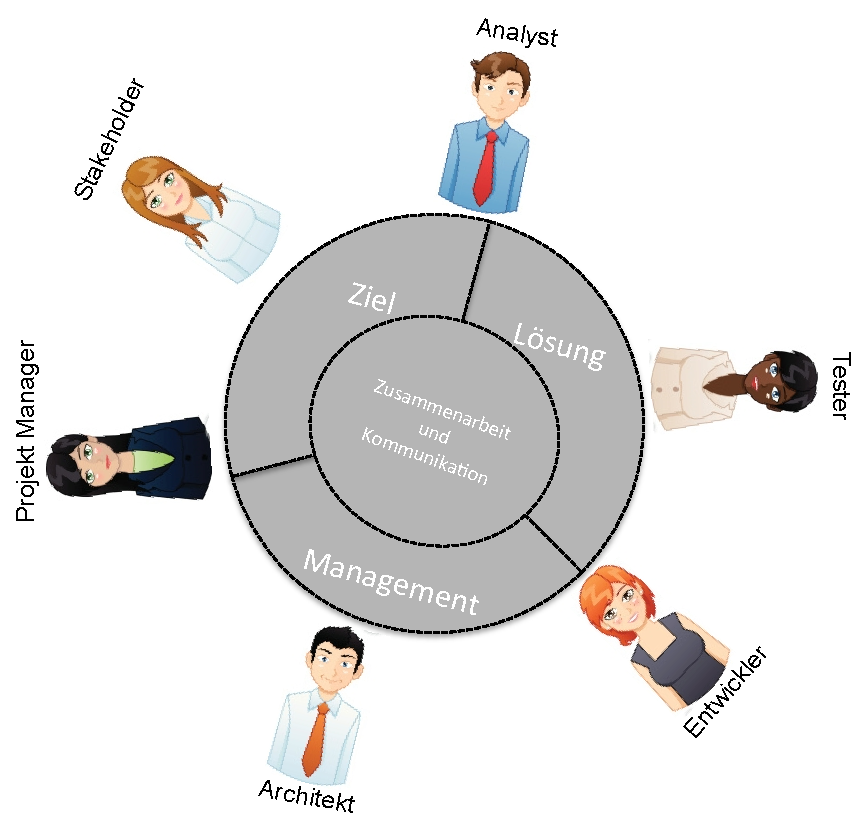
\includegraphics[scale=0.6]{RollenOpenUp} %pdf, jpg, png...
  \caption{Rollen in Open UP nach \cite{openup}}
  \label{fig:RollenOpenUp}
\end{center}
\end{figure}

Eine Task bezeichnet in Open UP die Arbeitseinheit einer Rolle, welche von dieser durchgeführt werden soll. Insgesamt gibt es 18 Tasks, die von den verschiedenen Rollen entweder als Hauptakteur (der Verantwortliche für die Durchführung der Aufgabe) oder als zusätzlicher Akteur (Unterstützung und Bereitstellung von Informationen, die in der Task- Ausführung verwendet werden), durchgeführt werden. Hierdurch wird der kollaborative Charakter von Open UP gefestigt \cite{eclipseopenup}.

Ein Artefakt ist etwas, das hergestellt, modifiziert oder durch eine Task verwendet wird. Rollen sind 
für die Erstellung und Aktualisierung von Artefakten verantwortlich. Artefakte stellen eine Versionskontrolle während des gesamten Projektlebenszyklus dar. Die 17 Artefakte in Open UP gelten als die wesentlichen Artefakte, welche ein Projekt verwenden sollte, um produkt- und projektbezogene Informationen zu erfassen. Die Informationen müssen hierbei nicht mit formalen Artefakten festgehalten werden. Dies kann auch informell, z.B. durch White-Boards oder Meeting-Notizen geschehen. Es können die Open UP Artefakte oder eigene Artefakte verwendet werden \cite{eclipseopenup}.

\subsection{Imperative Modellierung Open UP}

Nachfolgend werden einzelne Abschnitte des Open UP in der imperativen Prozessmodellierungssprache BPMN modelliert.

 \subsubsection{Phasen Open UP}

In Abbildung \ref{fig:OpenUpPhasen} sind die vier Phasen des Open UP modelliert. Da jede Phase in Iterationen mehrmals durchlaufen werden kann, gibt es nach jeder Phase ein XOR-Gateway, welches im Falle einer weiteren notwendigen Iteration zum Anfang der Phase zurückführt. Diese kann sodann erneut durchlaufen werden.

\begin{sidewaysfigure}[htp]
\begin{center}
  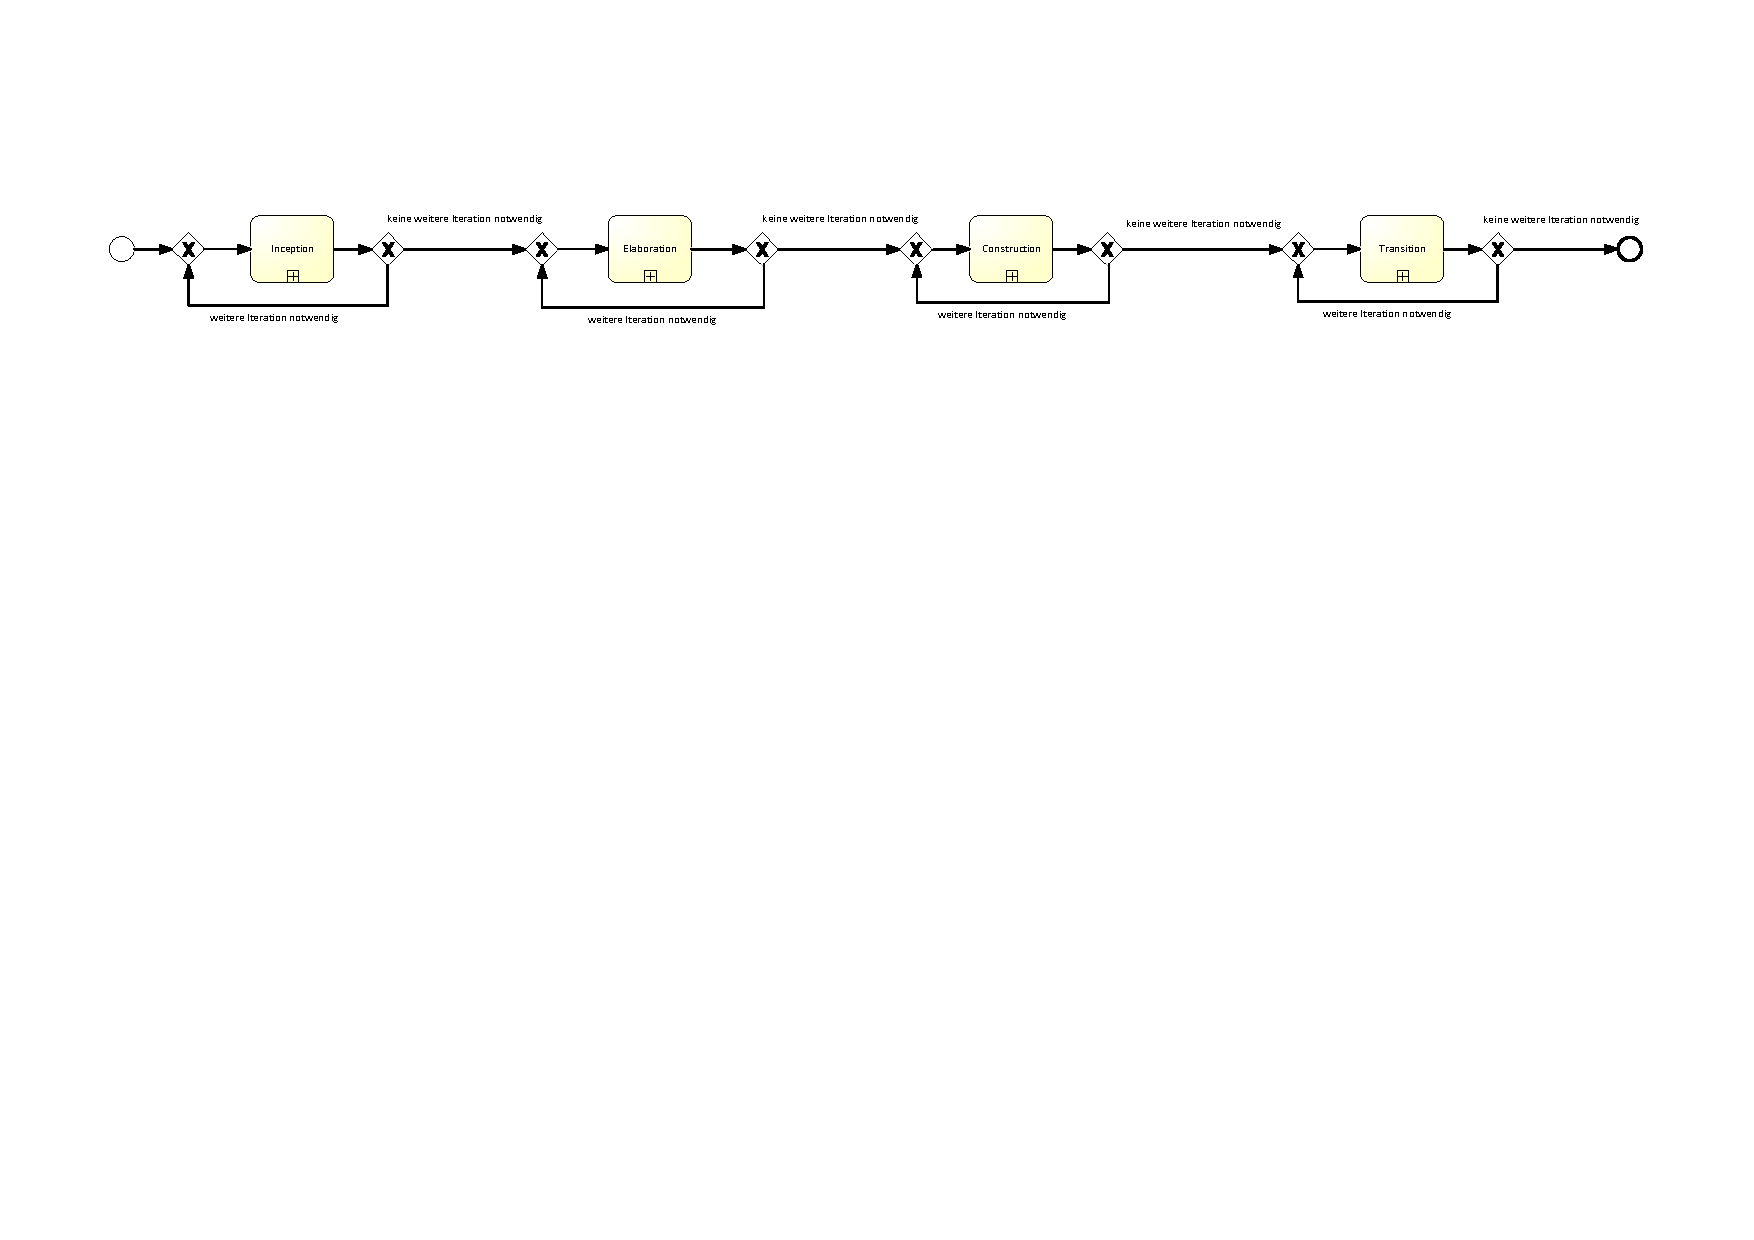
\includegraphics[width=\linewidth]{OpenUpPhasen} %pdf, jpg, png...
  \caption{Phasen Open UP- imperativ}
  \label{fig:OpenUpPhasen}
\end{center}
\end{sidewaysfigure}

Abbildung \ref{fig:OpenUpInception} zeigt die imperative Modellierung der Iteration Inception. Die Aktivität \grqq Projekt planen und managen \grqq \ kann parallel zu allen anderen Aktivitäten des Modells ausgeführt werden.\newline
Nach Ausführung der Aktivität \grqq Iteration planen\grqq \ werden die Aktivitäten \grqq Anforderungen identifizieren und aufbereiten\grqq \ und \grqq auf technisches Vorgehen einigen\grqq \ parallel zueinander ausgeführt.

\begin{figure}[htp]
\begin{center}
  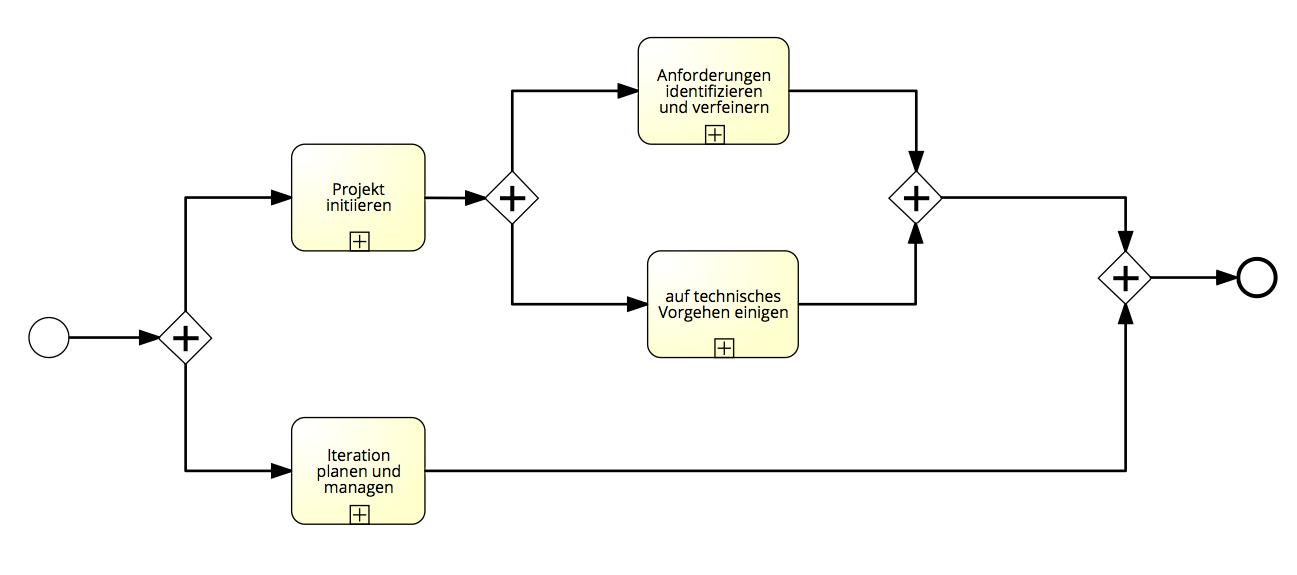
\includegraphics[scale=0.8]{OpenUpInception} %pdf, jpg, png...
  \caption{Phasen Open UP Unterprozess Inception- imperativ}
  \label{fig:OpenUpInception}
\end{center}
\end{figure}

In Abbildung \ref{fig:OpenUpElaboration} ist die imperative Modellierung der Iteration Elaboration abgebildet. Die sechs Aktivtäten \grqq Anforderungen identifizieren und verfeinern, Architektur entwickeln, Lösungsinkrement entwickeln, Lösung testen, Iteration planen und managen\grqq \ sowie \grqq weitere Aufgaben erledigen\grqq \ werden parallel zueinander ausgeführt.

\begin{figure}[htp]
\begin{center}
  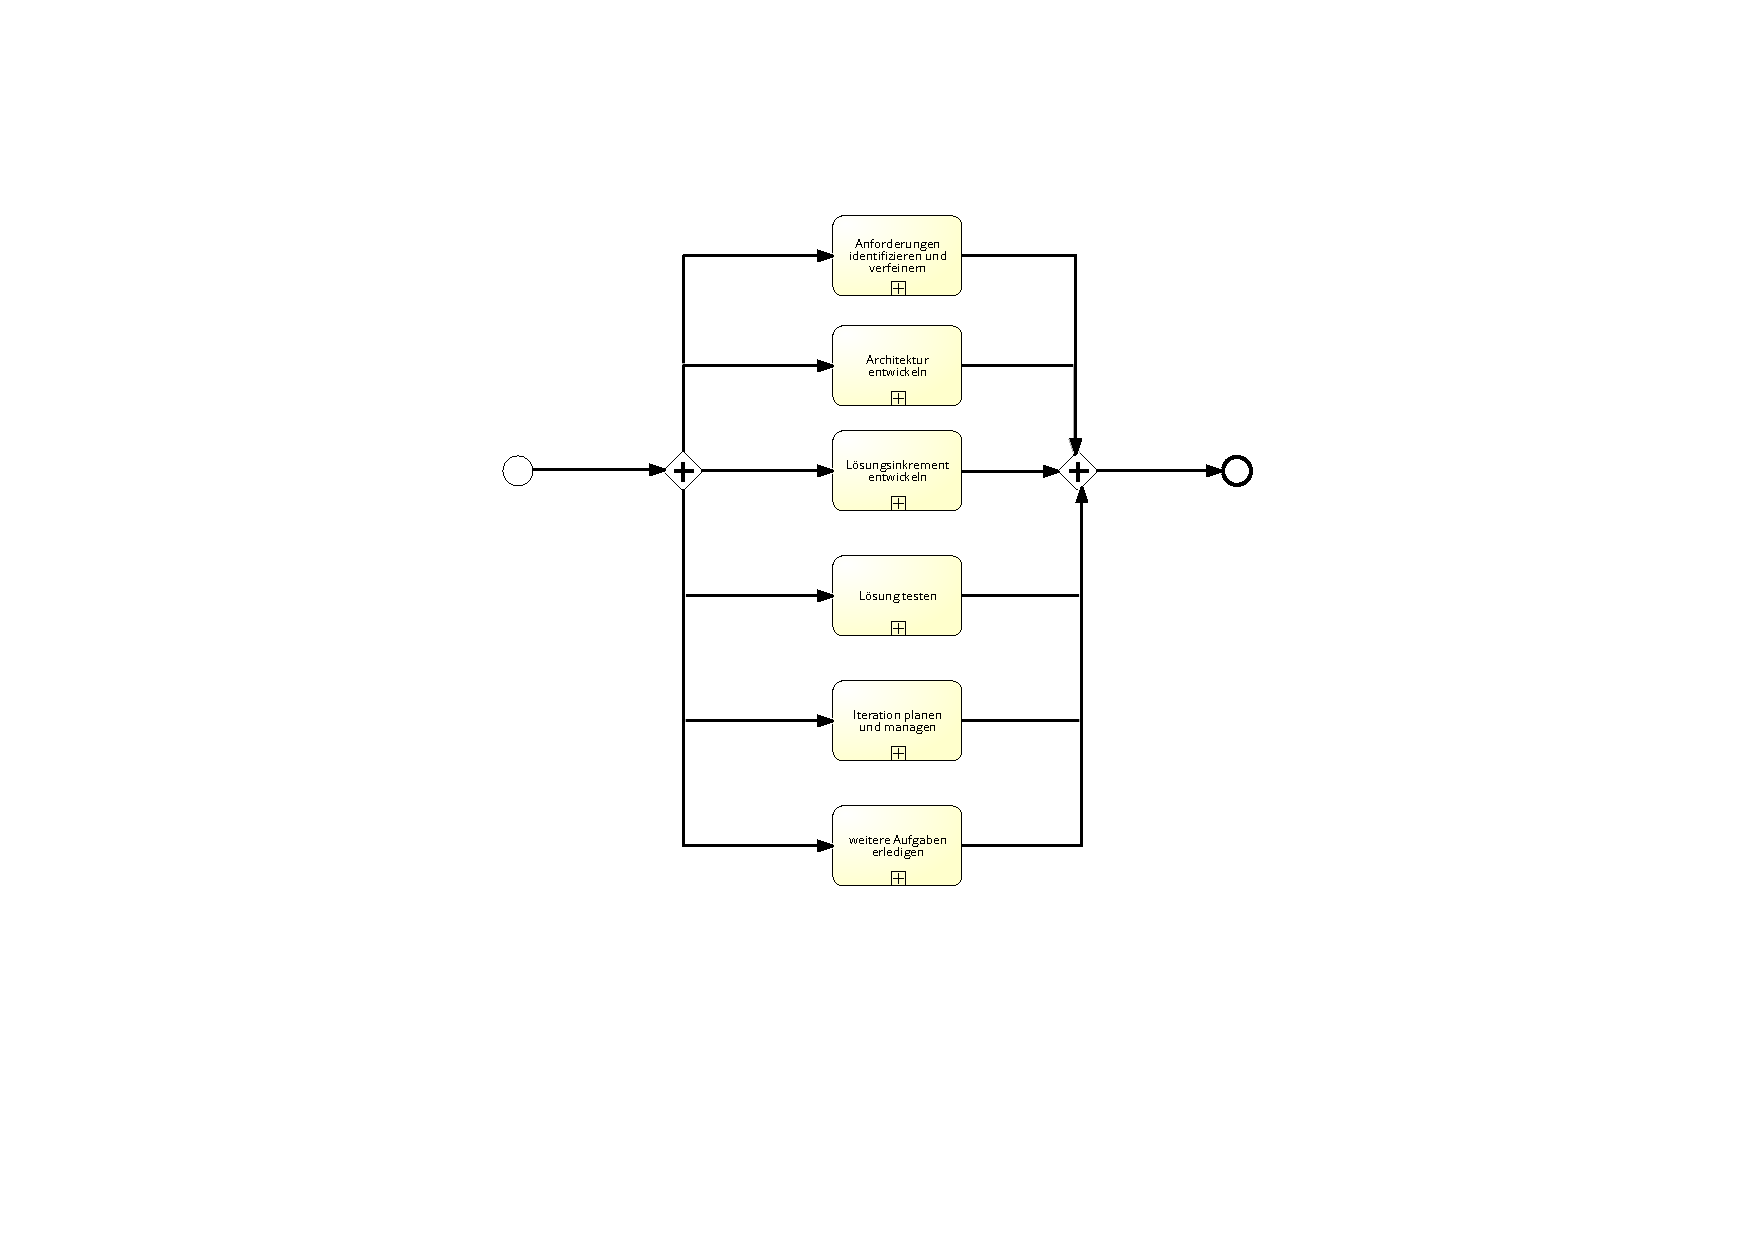
\includegraphics[scale=0.8]{OpenUpElaboration} %pdf, jpg, png...
  \caption{Phasen Open UP Unterprozess Elaboration- imperativ}
  \label{fig:OpenUpElaboration}
\end{center}
\end{figure}

Die imperative Modellierung der Iteration Construction kann Abbildung \ref{fig:OpenUpConstruction} entnommen werden. Hier werden die sechs Aktivitäten \grqq Anforderungen identifizieren und verfeinern, Lösungsinkrement entwickeln, Lösung testen, Iteration planen und managen, weitere Aufgaben erledigen und \grqq Produktdokumentation und Training erstellen\grqq \ nebeneinander parallel ausgeführt.
\begin{figure}[htp]
\begin{center}
  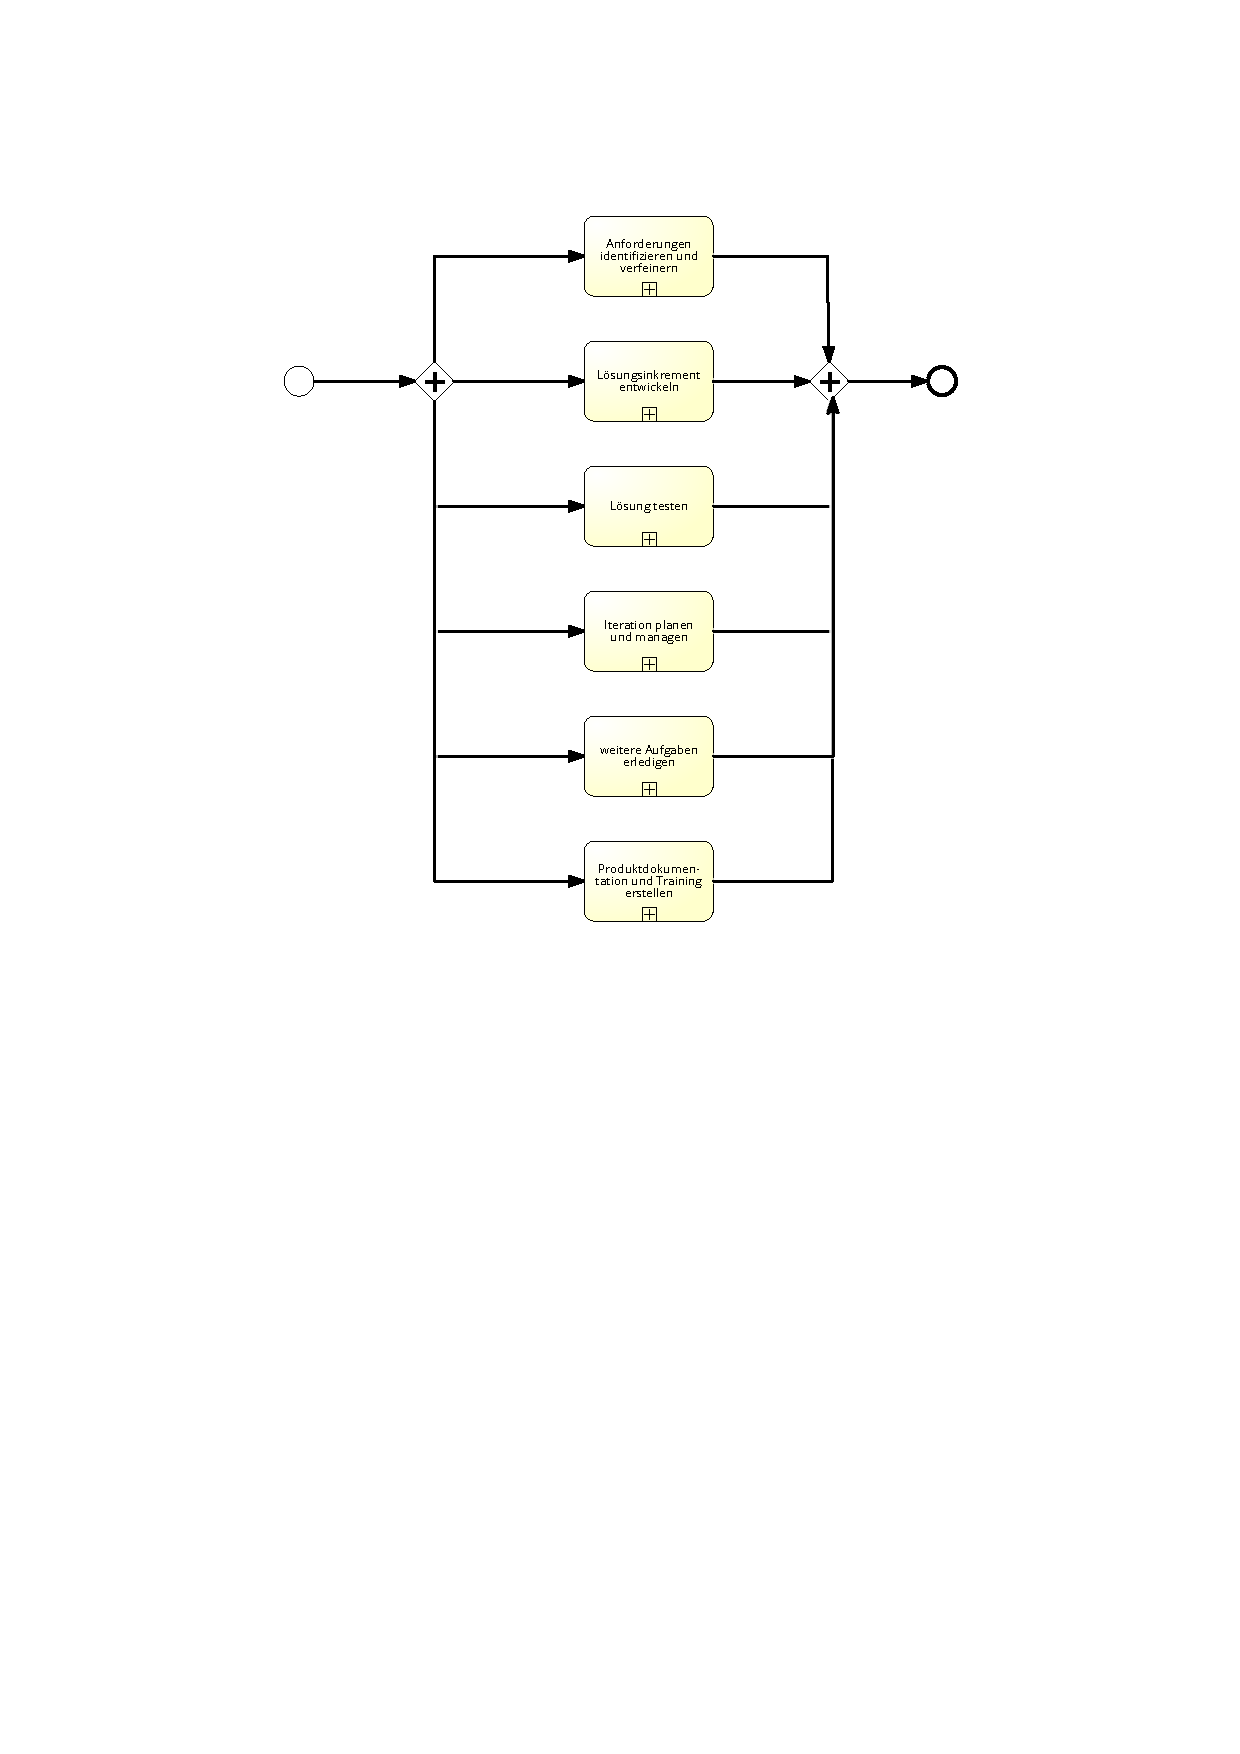
\includegraphics[scale=0.8]{OpenUpConstruction} %pdf, jpg, png...
  \caption{Phasen Open UP Unterprozess Construction- imperativ}
  \label{fig:OpenUpConstruction}
\end{center}
\end{figure}

Abbildung \ref{fig:OpenUpTransition} kann die imperative Modellierung der Iteration Transition entnommen werden. Die Phasen \grqq Anforderungen identifizieren und verfeinern, Produkt Training durchführen, Lösungsinkrement entwickeln, Lösung testen, Iteration planen und managen, weitere Aufgaben erledigen, Produktdokumentation und Training abschließen\grqq \ sowie \grqq Release deployen\grqq \ werden parallel zueinander ausgeführt.

\begin{figure}[htp]
\begin{center}
  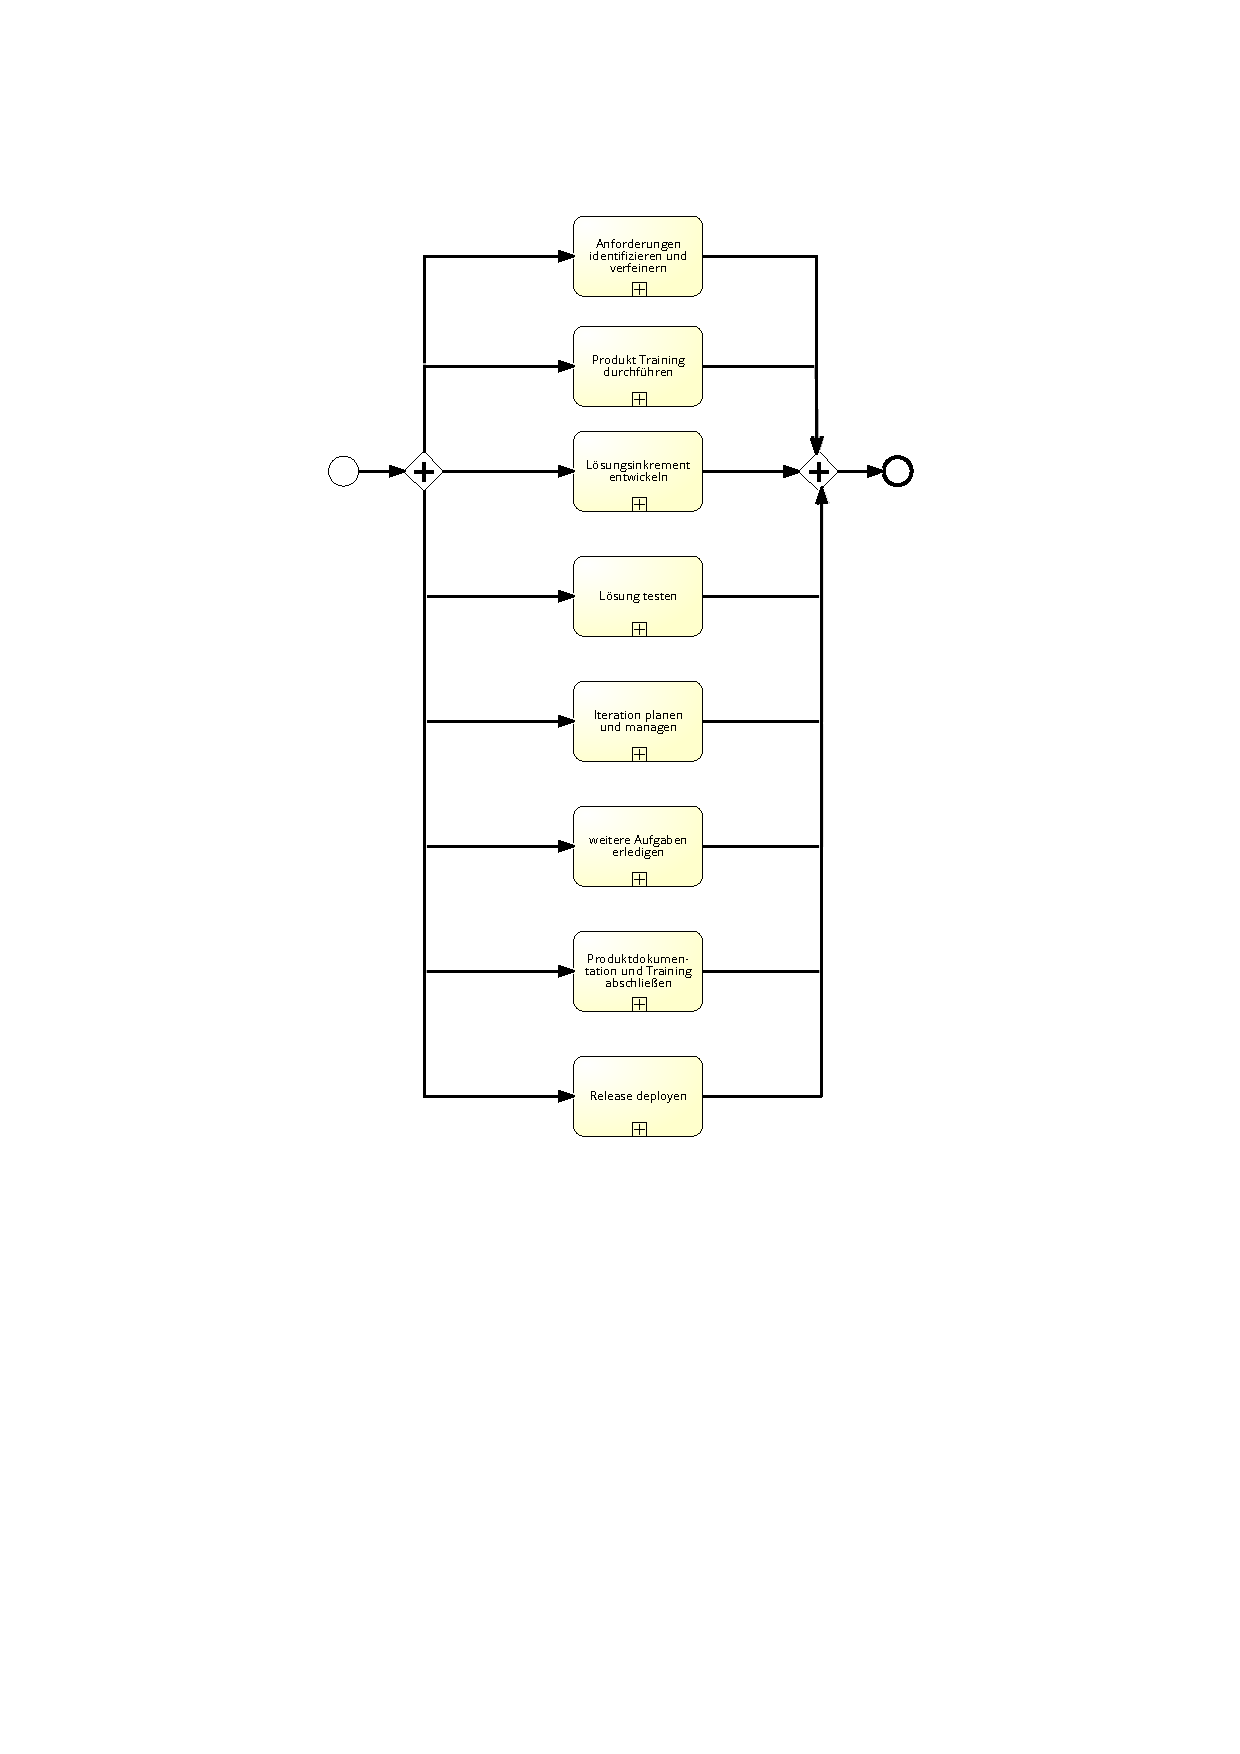
\includegraphics[scale=0.8]{OpenUpTransition} %pdf, jpg, png...
  \caption{Phasen Open UP Unterprozess Transition- imperativ}
  \label{fig:OpenUpTransition}
\end{center}
\end{figure}



Im weiteren Verlauf wird aus jeder der vier Iterationen Inception, Elaboration, Construction und Transition des Open UP jeweils ein repräsentativer Unterprozess modelliert, da die Abbildung aller Unterprozesse aus jeder Itaeration den Rahmen der Arbeit sprengen würde. \newline
Somit wird für die Iteration Inception der Unterprozess \grqq Iteration planen und managen\grqq, für die Iteration Elaboration der Unterprozess \grqq Anforderungen identifizieren und verfeinern, für die Iteration Construction der Unterprozess \grqq Release deployen\grqq \ und für die Iteration Transition der Unterprozess \grqq Produktdokumentation und Training erstellen\grqq \ modelliert. Außerdem wird der in den drei Phasen Elaboration, Construction und Transition wiederkehrende Unterprozess \grqq Lösungsinkrement entwickeln\grqq \ modelliert.

\subsubsection{Lösungsinkrement entwickeln}

Im Unterprozess \textit{Lösungsinkrement entwickeln} geht es um das Design, die Implementierung, das Testen und die Integration der Lösung für eine Anforderung in einem bestimmten Kontext. Sie tritt genauso viele Male auf, wie es Arbeitsaufgaben gibt, die in einer Iteration entwickelt werden müssen.
 Handelt es sich um eine nicht-triviale Veränderung, wird zunächst eine Lösung designt und anschließend ein Entwickeltest implementiert. Bei einer trivialen Änderung an der bestehenden Implementierung kann diese auch direkt in der bestehenden Architektur vorgenommen werden. \newline
 Sobald die Fragen der technischen Umsetzung geklärt sind, werden Entwicklertests implementiert, um die Implementierung zu verifizieren. Anschließend werden diese Entwicklertests ausgeführt.\newline
 Falls bei der Ausführung der Tests Fehler ersichtlich werden, muss eine Lösung für diesen Fehler implementiert werden und die Entwicklertests müssen erneut ausgeführt werden. Dies wird solange wiederholt, bis alle Tests bestanden sind.\newline
An dieser Stelle kann der Entwurf nochmals überdacht werden. Falls hier beschlossen wird, dass der Code überarbeitet werden muss, muss im Prozess zurückgegangen werden und erneut eine Lösung designt werden, da eine Änderung des Codes die Implementation und die Entwicklertests beeinflussen könnte.\newline
 Da es am Besten ist, die Implementierungsteile so klein wie möglich zu halten, sollte zunächst eine kleine Design-Lösung für einen Teil der Arbeitsaufgabe entwickelt werden. Anschließend sollte dies für weitere kleine Teile solange wiederholt werden, bis die gesamte Arbeitsaufgabe implementiert ist. \newline
 In Abbildung \ref{fig:Dev} ist die imperative Modellierung von \grqq Lösungsinkrement entwickeln\grqq \ abgebildet.\newline
 Die XOR-Verknüpfung am Anfang führt im Falle einer trivialen Änderung zur sofortigen Ausführung der Aktivität \textit{Entwicklertest implementieren}. Falls es sich jedoch um eine typische Änderung handelt, muss zuvor die Aktivität \grqq Lösung designen\grqq \ ausgeführt werden. Im Anschluss an \grqq Entwicklertest implementieren\grqq \ muss die Aktivität \grqq Entwicklertest ausführen\grqq \ durchgeführt werden.\newline
 Hiernach wird im Falle eines fehlgeschlagenen Tests zunächst eine \grqq Lösung implementiert\grqq \ und anschließend erneut der \grqq Entwicklertest ausgeführt\grqq. \newline
 Wenn der Test bestanden ist, muss am XOR-Gateway entschieden werden, ob der Code gut designt ist. Falls nein, muss erneut eine Lösung designt werden. Falls doch, kann der Code integriert werden. Ist die Arbeit vollständig erledigt, so ist der Prozess beendet. Wenn jedoch noch weitere Arbeit vorhanden ist, beginnt er von vorne.
 
 
\begin{figure}[htp]
\begin{center}
  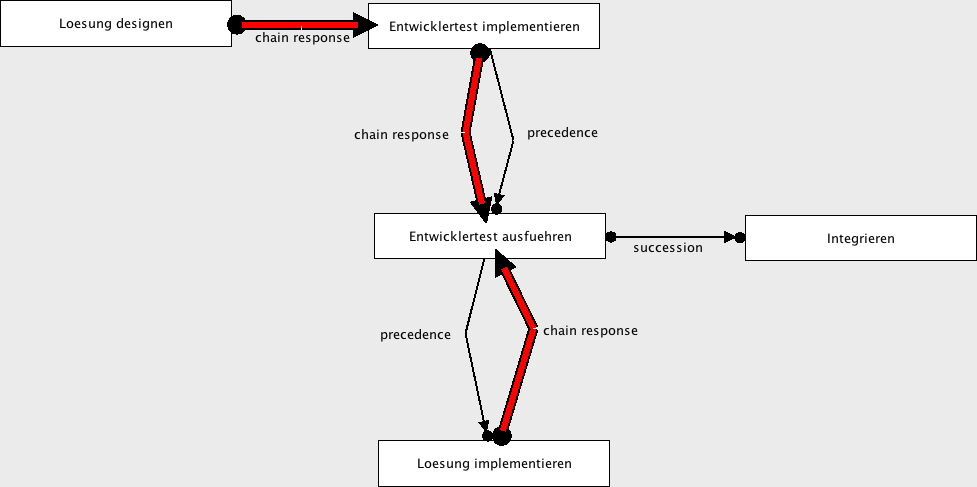
\includegraphics[width=\linewidth]{DevelopSolution} %pdf, jpg, png...
  \caption{Lösungsinkrement entwickeln imperativ}
  \label{fig:Dev}
\end{center}
\end{figure}

\subsubsection{Iteration planen und managen- Inception}

Die Aktivität \grqq Iteration planen und managen\grqq \ wird während des gesamten Projektlebenszyklus ausgeführt. Ihr Ziel ist es, Risiken und Probleme früh genug zu identifizieren, damit diese entschärft werden können, um die Ziele für die Iteration festzulegen und das Team dabei zu unterstützen, diese zu erreichen.\newline
Die Iteration wird durch den Projektmanager und das Team gestartet. Hier findet die Priorisierung der Arbeit für eine gegebene Iteration statt. Der Projektmanager, die Stakeholder und die Teammitglieder einigen sich darauf, was während der Iteration zu entwickeln ist.\newline
Die Teammitglieder melden sich für die Arbeitsaufgaben, die während der Iteration entwickelt werden müssen. Anschließend teilt sich jedes Teammitglied seine Arbeitsaufgaben selbstständig in Arbeitseinheiten ein und schätzt den Aufwand hierfür ab.\newline
Während der Iteration trifft sich das Team regelmäßig, um den aktuellen Stand der Arbeit und eventuelle Probleme zu besprechen. \newline
Abbildung \ref{fig:PlanAndManageIterationInception-2} zeigt die imperative Modellierung von \grqq Iteration planen und managen\grqq. \newline
Vom Projektmanager sind hierbei nacheinander die Aktivitäten \grqq Iteration planen, Umgebung vorbereiten, Iteration managen\grqq \ und \grqq Ergebnisse festlegen\grqq \ durchzuführen und das Team muss nacheinander die Aktivitäten \grqq Arbeitsaufgaben aussuchen, Arbeitsaufgaben in Entwicklungsaufgaben einteilen\grqq \ sowie \grqq Aufwand abschätzen\grqq \ ausführen. Hierbei gehen jeweils die Artefakte \grqq Arbeitseinheiten-Liste, Iterationsplan\grqq \ und \grqq Risiko-Liste\grqq \ in verschieden Aktivitäten als Input ein und kommen eventuell verändert als Output wieder heraus. \newline
Die Aktivität \grqq Umgebung vorbereiten\grqq \ ist als Unterprozess in Abbildung \ref{fig:Umgebungvorbereiten} dargestellt. Hier müssen vom Projektmanager die Aktivitäten \grqq Prozess Maßschneidern\grqq \ und \grqq Prozess deployen\grqq \ sequentiell erledigt werden, während der Tool Spezialist die Aufgaben \grqq Tools aufsetzen\grqq \ und \grqq Tool-Konfiguration und Implementation verifizieren\grqq \ zu erledigen hat.


\begin{figure}[!htbp]
\begin{center}
  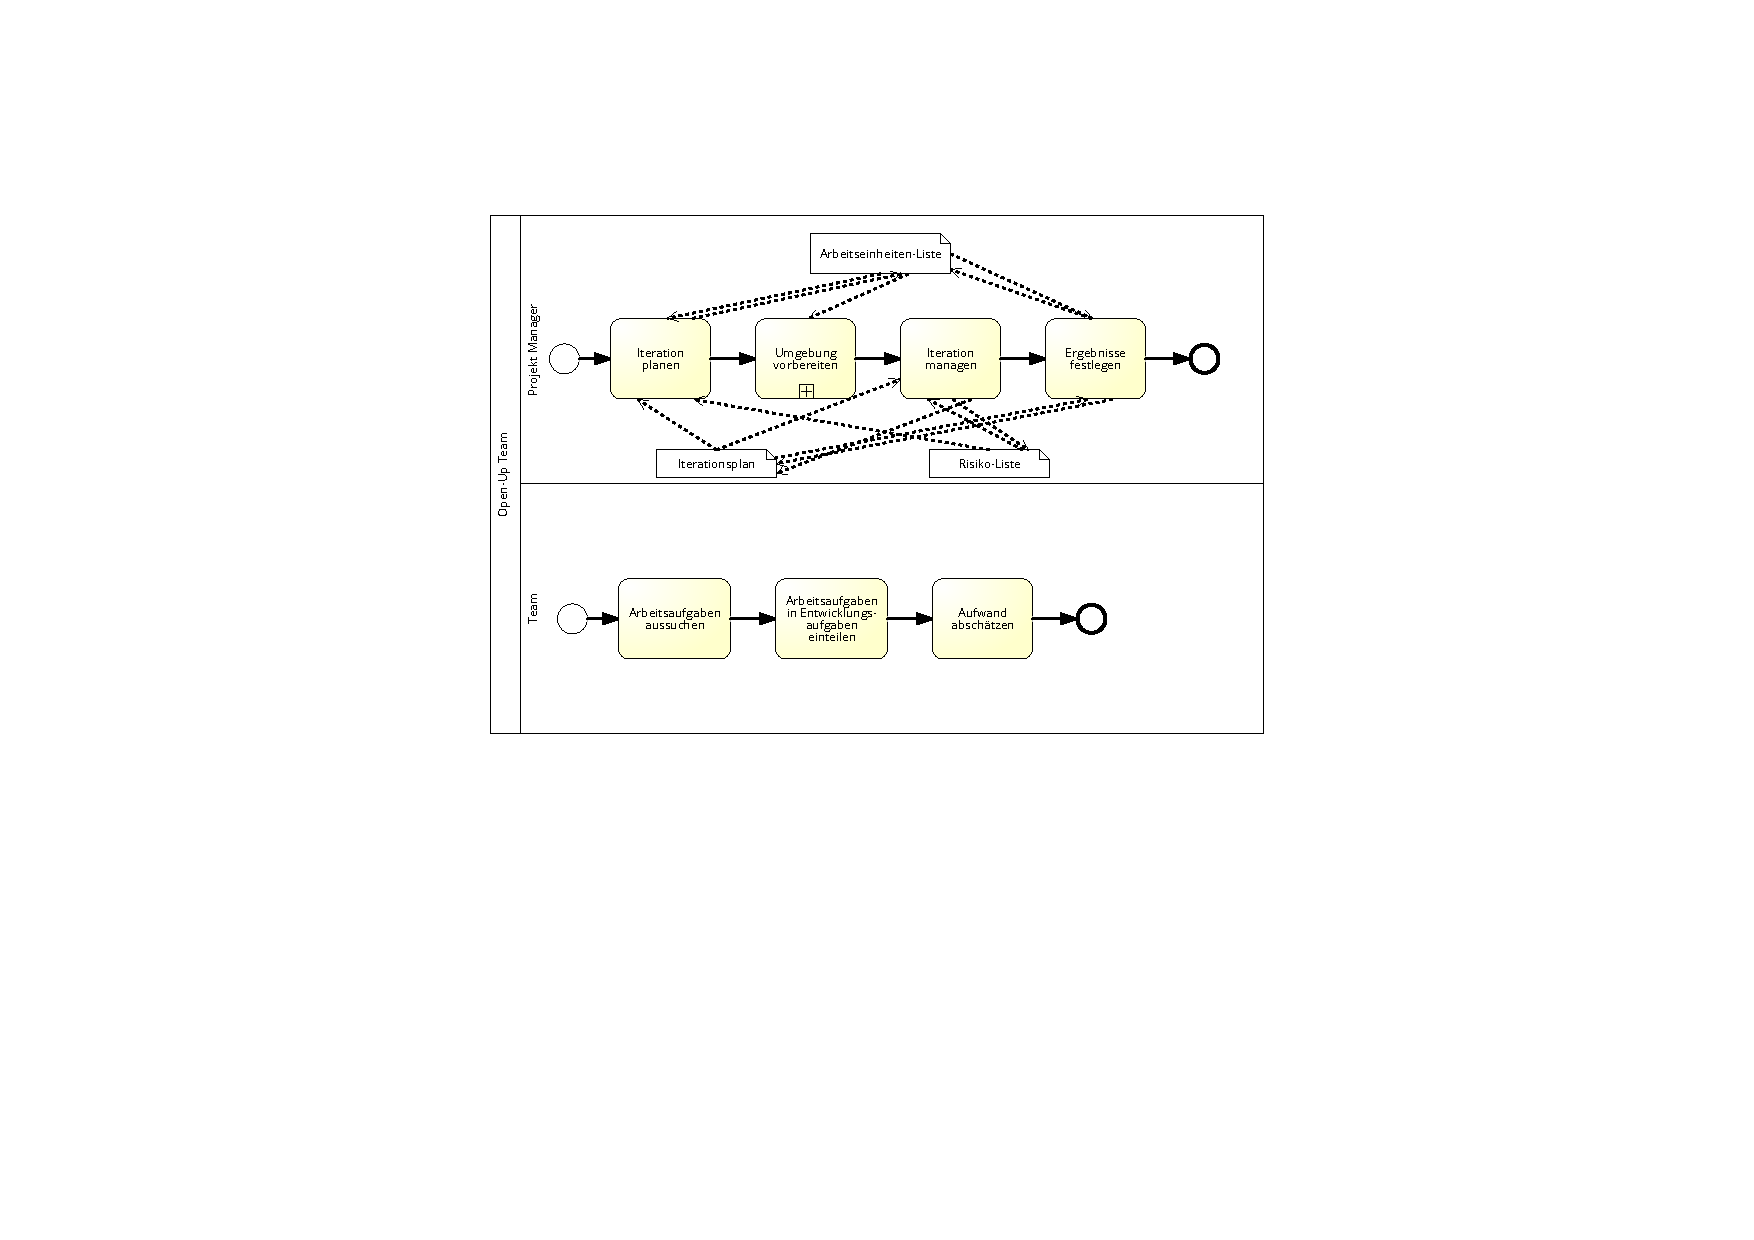
\includegraphics[scale=0.7]{PlanAndManageIterationInception-2} %pdf, jpg, png...
  \caption{Iteration planen und managen imperativ -Inception}
  \label{fig:PlanAndManageIterationInception-2}
\end{center}
\end{figure}

\begin{figure}[!htbp]
\begin{center}
  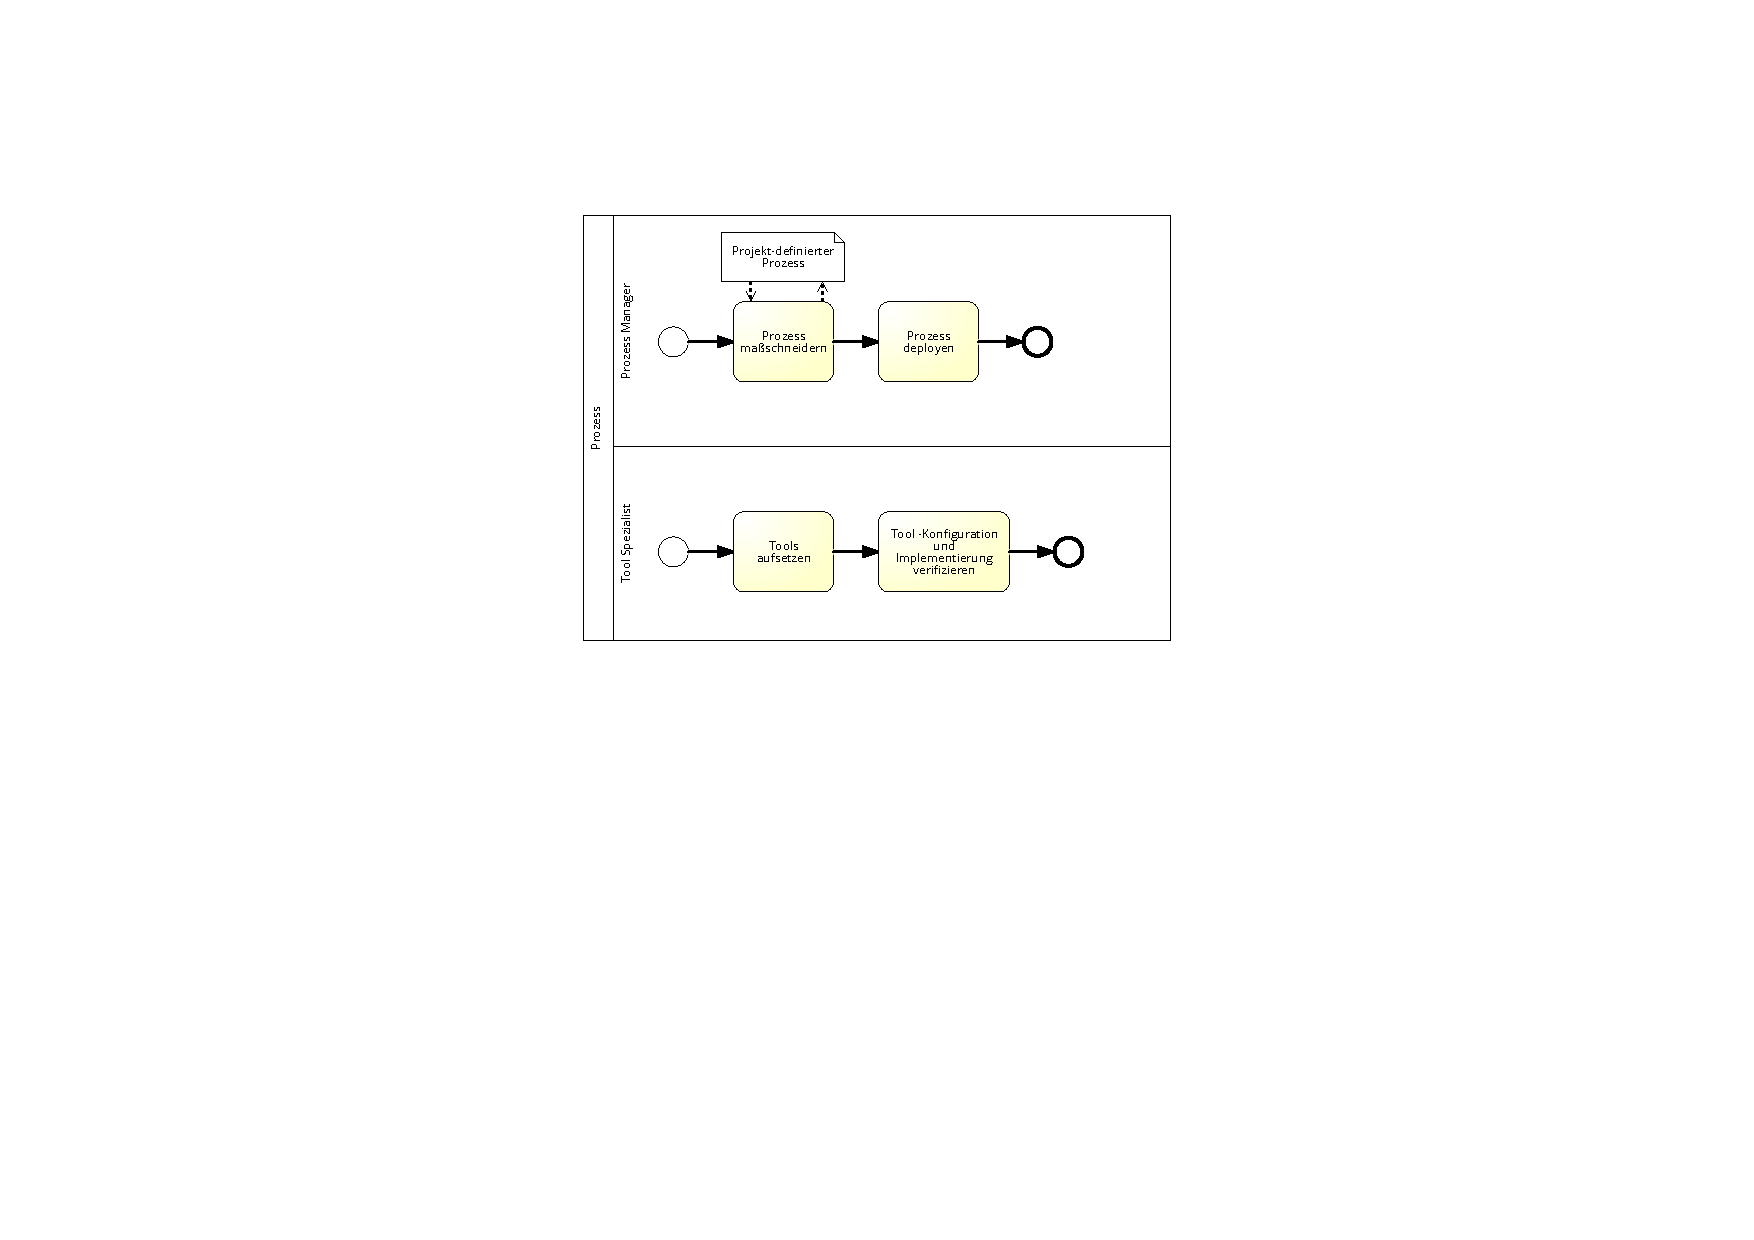
\includegraphics[scale=0.7]{Umgebungvorbereiten} %pdf, jpg, png...
  \caption{Iteration planen und managen imperativ -Inception Unterprozess Umgebung vorbereiten} 
  \label{fig:Umgebungvorbereiten}
\end{center}
\end{figure}

\clearpage


\subsubsection{Anforderungen identifizieren und verfeinern}
 Der Unterprozess \textit{Anforderungen identifizieren und verfeinern} beschreibt die Aufgaben, welche durchzuführen sind, um die Anforderungen eines Systems zu sammeln, zu analysieren und zu validieren bevor die Implementierung und die Validierung stattfinden. Sie wird in Zusammenarbeit mit Stakeholdern und dem gesamten Entwicklungsteam ausgeführt, um sicher zu gehen, dass klare, konsistente, korrekte und nachprüfbare Anforderungen vorhanden sind.\newline
 In der Phase Elaboration liegt der Fokus auf der Definition der Lösung. Hierfür müssen diejenigen Anforderungen gefunden werden, welche für die Stakeholder am wichtigsten sind die besonders herausfordernd oder sogar riskant sind oder eine große Bedeutung für die Architektur haben.\newline
 Dafür ist es notwendig, zunächst die funktionalen und nicht-funktionalen Anforderungen an das System zu erheben. Genau diese Anforderungen stellen dann die Basis für die Kommunikation und die Übereinstimmung zwischen den Stakeholdern und dem Entwicklungsteam dar, in Bezug auf was das System können muss, um die Wünsche der Stakeholder zu erfüllen.\newline
 Weiterhin müssen die Use-Case-Szenarien und die systemweiten Anforderungen ausführlich genug beschrieben werden, um sicher zu gehen, dass die Anforderungen richtig verstanden wurden und dass diese mit den Erwartungen der Stakeholder übereinstimmen.\newline
 Zudem müssen Testfälle und Testdaten für die Anforderungen entwickelt werden, um ein gemeinsames Verständnis für die spezifischen Bedingungen, die die Lösung erfüllen muss, zu erreichen.
 In Abbildung \ref{fig:IdentifyAndOutlineKlein} ist die imperative Modellierung von \grqq Anforderungen identifizieren und verfeinern\grqq \ abgebildet. \newline
 Zunächst muss der Analyst die \grqq Anforderungen identifizieren und abgrenzen\grqq, bevor er anschließend die \grqq Use-Case-Szenarien detaillieren\grqq kann. Daraufhin muss er die \grqq Systemweiten Anforderungen detaillieren\grqq, damit der Tester anschließend die \grqq Testfälle erstellen\grqq kann.\newline
 Hier gehen bei den verschiedenen Aktivitäten die Artefakte \grqq Arbeitseinheitenliste\grqq, \grqq Use Case\grqq, \grqq Glossar\grqq, \grqq Systemweite Anforderungen\grqq, \grqq Use case Modell\grqq, \grqq Technische Spezifikation\grqq \ und \grqq Testfall\grqq \ als Input hinein, bzw. als Output heraus.
 
\begin{figure}[[!htbp]
\begin{center}
  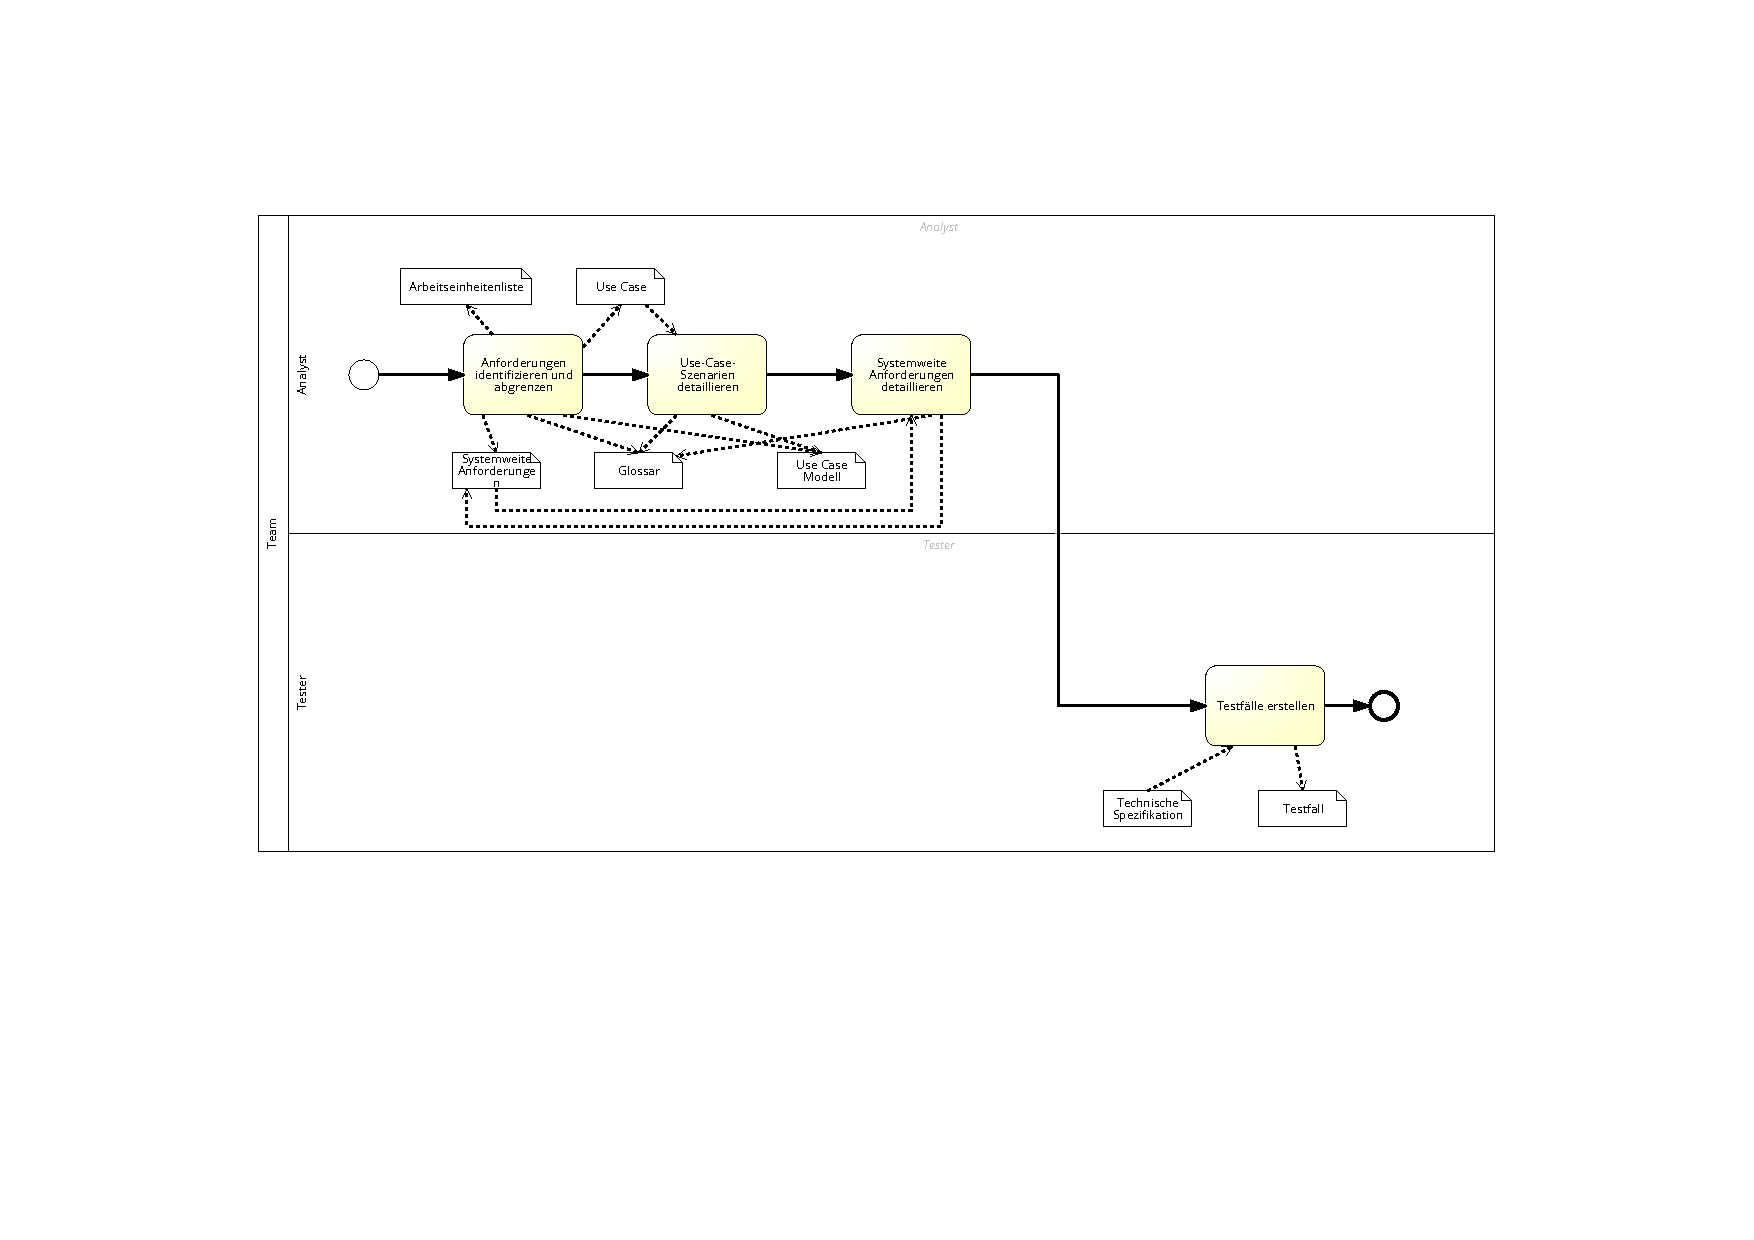
\includegraphics[width=\linewidth]{IdentifyAndOutlineKlein} %pdf, jpg, png...
  \caption{Anforderungen identifizieren und verfeinern-Elaboration}
  \label{fig:IdentifyAndOutlineKlein}
\end{center}
\end{figure}


\subsubsection{Produktdokumentation und Training erstellen-Construction}
 Das Ziel des Unterprozesses \grqq Produktdokumentation und Training erstellen\grqq \ ist es, die Produktdokumentation und Trainingsmaterial vorzubereiten. Da die Produktdokumentation oftmals erst nach Abschluss der Entwicklungstätigkeiten erstellt wird, muss sichergestellt werden, dass die Funktionen die während einer Release entwickelt werden klar dokumentiert werden, solange die Funktionalität noch frisch in den Köpfen der Teammitglieder vorhanden ist.\newline
 Hierfür ist es notwendig, dass genug Informationen über die Funktionen, die in einer bestimmten Release entwickelt wurden, dokumentiert werden, um dem Kunden während der gesamten Lebenszeit des Produkts nützlich zu sein.\newline
 Weiterhin müssen den Endnutzern hilfreiche Informationen bereit gestellt werden in Form von Benutzerhandbüchern, Tutorials, häufig gestellte Fragen (FAQs), Online-Hilfedateien, Installationsanweisungen und Betriebsabläufe. \newline
 Zudem muss sichergestellt werden, dass diejenigen, die mit der Unterstützung des Systems beauftragt sind, genug Informationen über das Produkt haben, um ihre Arbeit effektiv durchzuführen, nachdem das Produkt produktiv gegangen ist. Außerdem muss die Einführung des Produkts ermöglicht werden und dessen ordnungsgemäße Verwendung gewährleistet werden.\newline
 
 Die imperative Modellierung von \grqq Produktdokumentation und Training erstellen\grqq \ kann Abbildung \ref{fig:DevelopProductDocumentationKlein} entnommen werden.\newline
 Hier sind vom technischen Schreiber nacheinander die Aktivitäten \grqq Produktdokumentation erstellen\grqq, \grqq Benutzerdokumentation erstellen\grqq, \grqq Unterstützungsdokumentation erstellen\grqq \ und \grqq Trainingsmaterial erstellen\grqq \ auszuführen. Aus den jeweiligen Aktivitäten entstehen sodann die Artefakte \grqq Produktdokumentation, Benutzerdokumentation, Unterstützungsdokumentation\grqq \ und \grqq Trainingsmaterial\grqq.
 
\begin{figure}[!htbp]
\begin{center}
  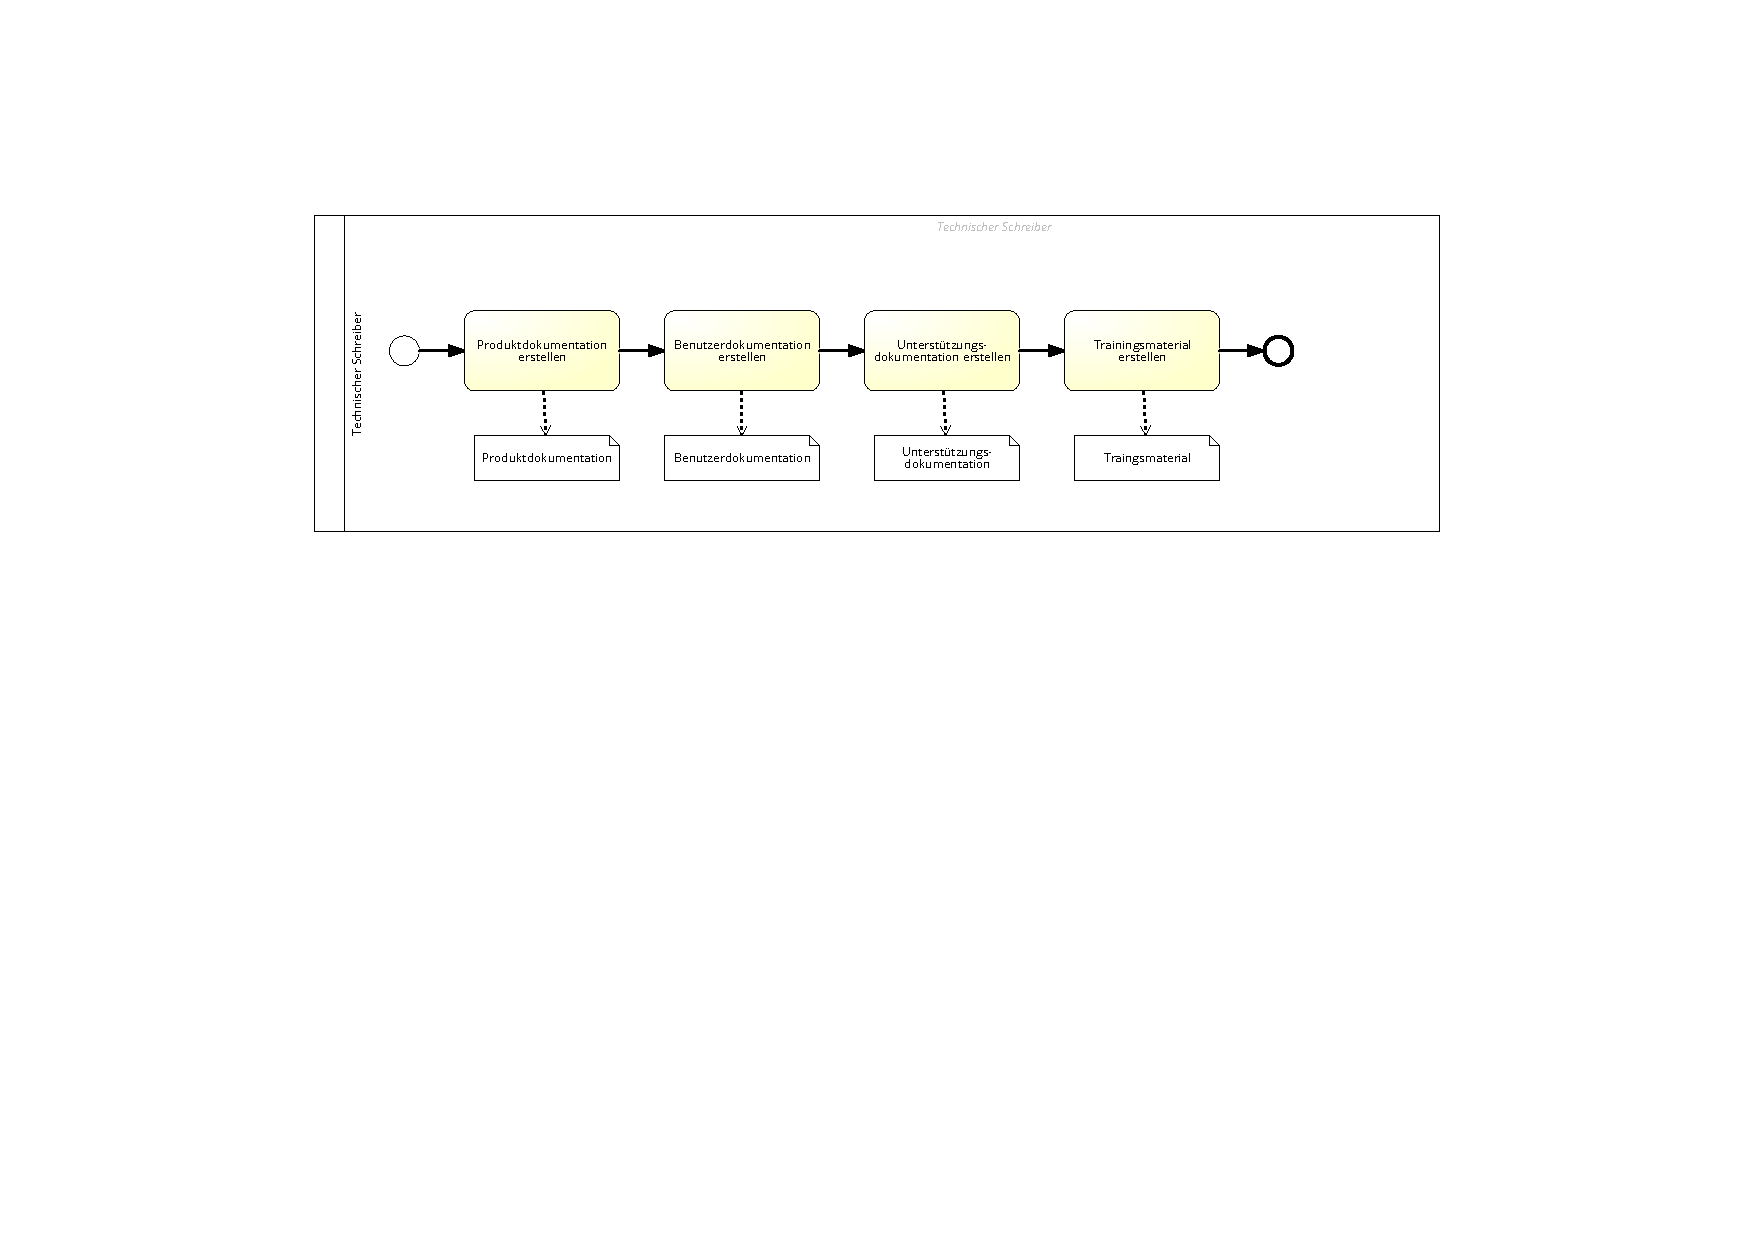
\includegraphics[width=\linewidth]{DevelopProductDocumentationKlein} %pdf, jpg, png...
  \caption{Produktdokumentation und Training erstellen - Construction}
  \label{fig:DevelopProductDocumentationKlein}
\end{center}
\end{figure}


\subsubsection{Release deployen-Transition}


Das Ergebnis dieses Unterprozesses ist die Release eines Sets von integrierten Komponenten in der Integrationsumgebung. Hierfür ist es notwendig, ein komplettes, bereitstellungsfähiges Paket zu erstellen, welches vom Deployment Engineer in die Bereitstellungsumgebung releast werden kann.\newline
 Außerdem muss sichergestellt werden, dass der Roll-Out aus klaren, geprüften und wiederholbaren Anweisungen besteht und das Risiko eines Bereitstellungsfehlers muss minimiert werden. \newline
 Zudem muss sichergestellt werden, dass eine Release zu keinen ungewollten Unterbrechungen im Ablauf in der Produktionsumgebung führt. Falls eine Release Probleme verursacht oder sie von den Stakeholdern als untauglich empfunden wird, muss diese Release von der Produktionsumgebung so schnell wie möglich entfernt werden. Zusätzlich muss dafür gesorgt werden, dass Informationen über eine anstehende Release weitest möglich verteilt werden.\newline
 
  Abbildung \ref{fig:DeployReleaseTransitionKlein} zeigt die imperative Modellierung von\grqq Release deployen\grqq.
  Somit muss der Entwickler zunächst die \grqq Release zusammenstellen\grqq, bevor der Deployment Engineer nacheinander die Aktivitäten \grqq Deploymentplan ausführen\grqq \ und \grqq erfolgreiches Deployment sicherstellen\grqq \ ausführt. Falls das Deployment erfolgreich ist, wird gleich anschließend die Aktivität \grqq Releasemitteilungen übermitteln\grqq \ ausgeführt. Ist das Deployment nicht erfolgreich, muss zunächst die Aktivität \grqq Backoutplan ausführen\grqq \ erledigt werden und erst danach die Aktivität \grqq Releasemitteilungen übermitteln\grqq \ ausgeführt werden.


\begin{figure}[!htbp]
\begin{center}
  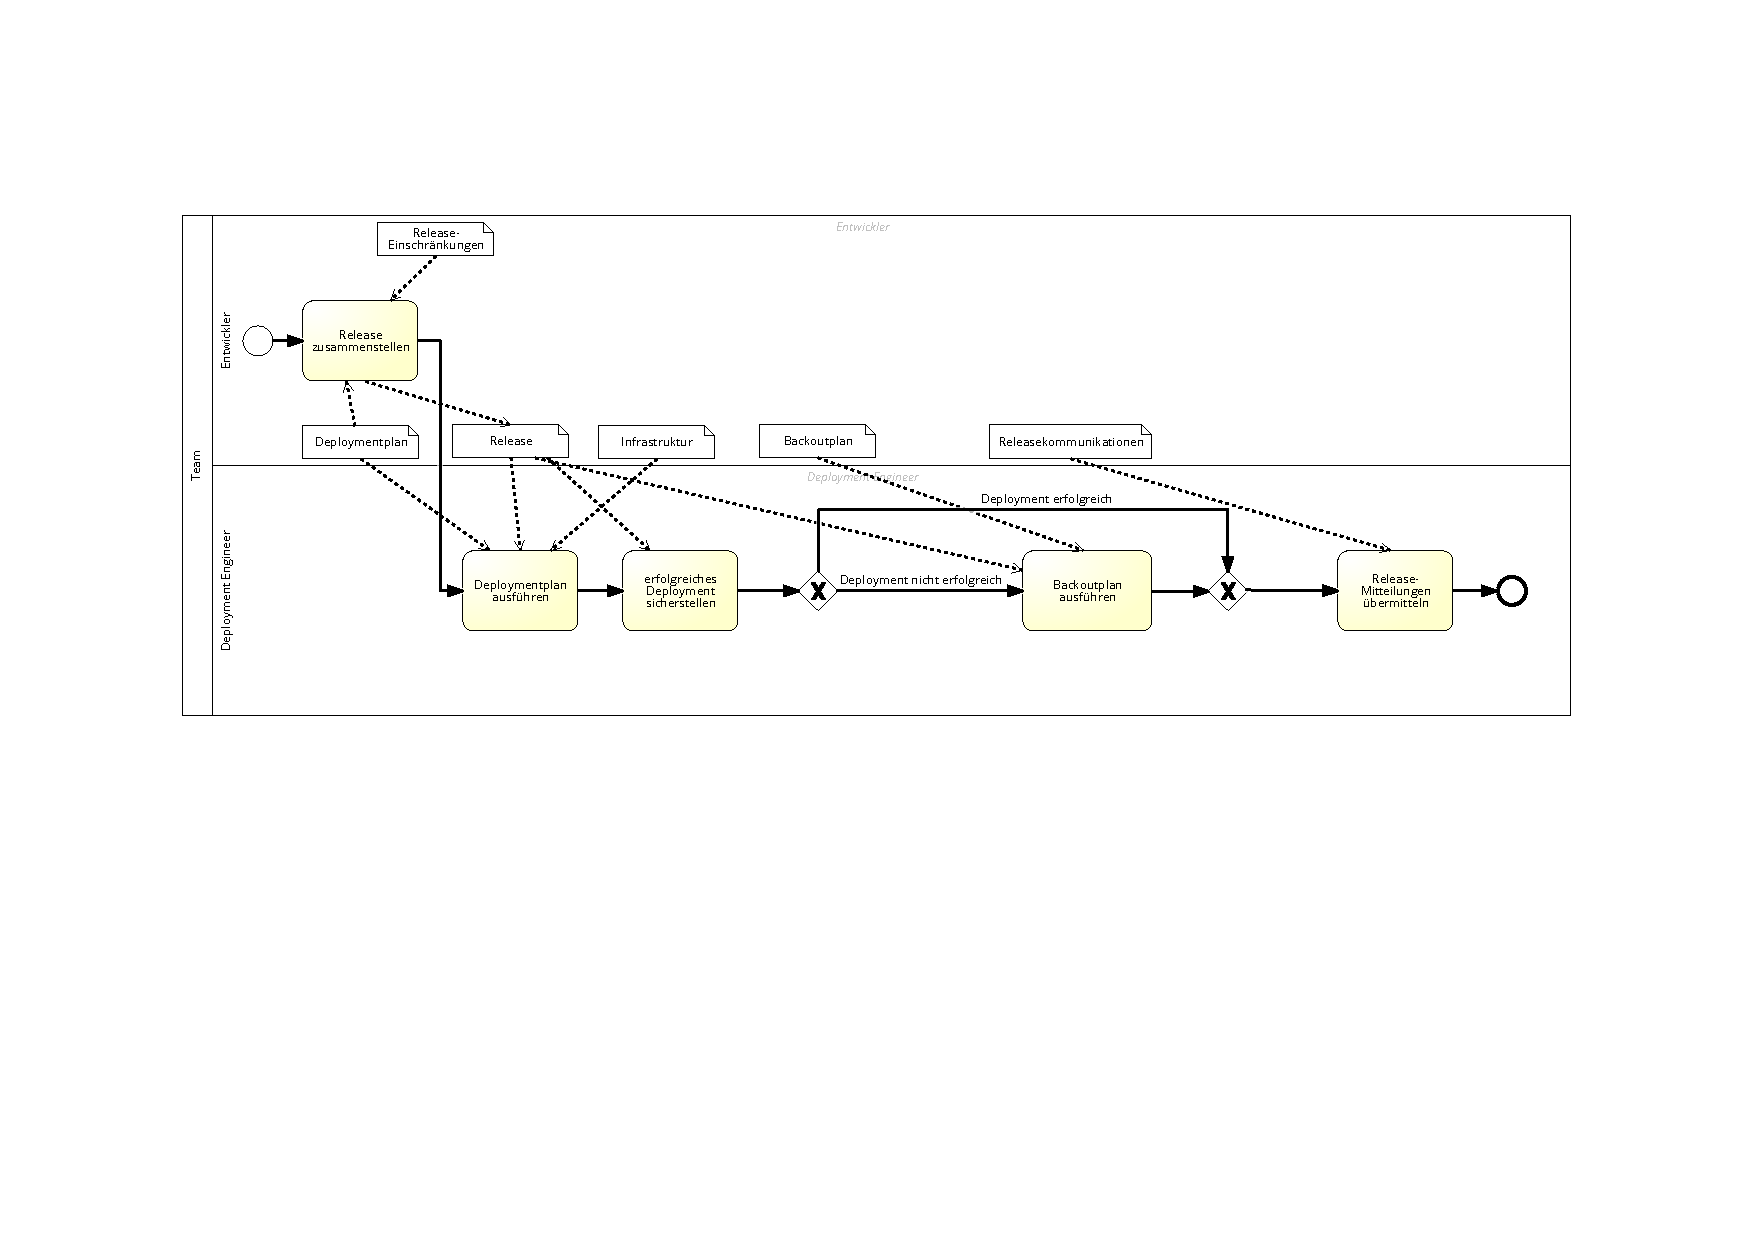
\includegraphics[width=\linewidth]{DeployReleaseTransitionKlein} %pdf, jpg, png...
  \caption{Release deployen-Transition}
  \label{fig:DeployReleaseTransitionKlein}
\end{center}
\end{figure}



\clearpage

\subsection{Deklarative Modellierung Open UP}




\subsubsection{Phasen des Open UP}


In Abbildung \ref{fig:OpenUpPhasenDec} sind die vier Phasen des Open UP deklarativ modelliert. Jede Phase kann in Iterationen mehrmals durchlaufen werden. Aus diesem Grund sind die vier Phasen durch das Constraint \textit{succesion} miteinander verbunden. Hierdurch wird gewährleistet, dass jede Phase so oft ausgeführt werden kann, wie nötig, aber dass ebenfalls die Reihenfolge eingehalten wird. So kann z.B. die Phase Elaboration erst durchlaufen werden, nachdem die Phase Inception durchlaufen wurde.
\begin{figure}[htp]
\begin{center}
  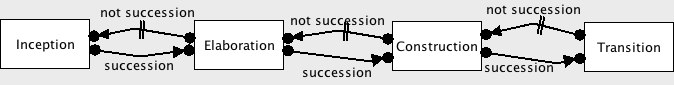
\includegraphics[width=\linewidth]{OpenUpPhasenDec} %pdf, jpg, png...
  \caption{Phasen Open UP- deklarativ}
  \label{fig:OpenUpPhasenDec}
\end{center}
\end{figure}




Abbildung \ref{fig:InceptionDecUnter} zeigt die deklarative Modellierung der Iteration Inception. Die Aktivität \textit{Projekt planen und managen} kann parallel zu allen anderen Aktivitäten des Modells ausgeführt werden.\newline
Nach Ausführung der Aktivität \grqq Iteration planen\grqq \ werden die Aktivitäten \grqq Anforderungen identifizieren und aufbereiten\grqq \ und \grqq auf technisches Vorgehen einigen\grqq \ parallel zueinander ausgeführt. Aus diesem Grund sind die Aktivitäten \grqq Anforderungen identifizieren und aufbereiten\grqq \ und \grqq auf technisches Vorgehen einigen\grqq \ mit der Aktivität \grqq Projekt planen und managen\grqq \ durch das Constraint \textit{succession} verbunden, da sie erst nach deren Ausführung ausgeführt werden dürfen und auch ausgeführt werden müssen. \newline

\begin{figure}[htp]
\begin{center}
  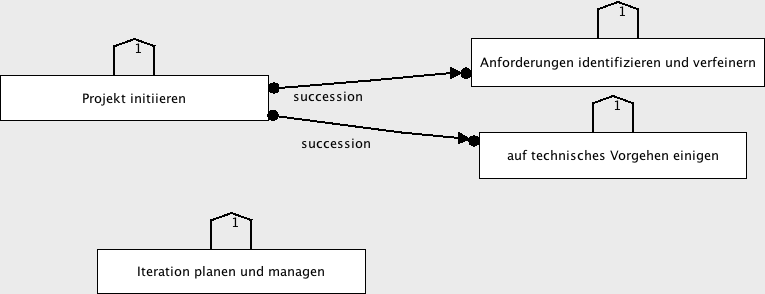
\includegraphics[width=\linewidth]{InceptionDecUnter} %pdf, jpg, png...
  \caption{Phasen Open UP Unterprozess Inception- deklarativ}
  \label{fig:InceptionDecUnter}
\end{center}
\end{figure}

In Abbildung \ref{fig:ElaborationDecUnter} ist die deklarative Modellierung der Iteration Elaboration abgebildet. Die sechs Aktivtäten\grqq Anforderungen identifizieren und verfeinern, Architektur entwickeln, Lösungsinkrement entwickeln, Lösung testen, Iteration planen und managen\grqq \ sowie \grqq weitere Aufgaben erledigen\grqq \ werden parallel zueinander ausgeführt. Aus diesem Grund befindet sich lediglich das Constraint \textit{Ecactly 1} an jeder Aktivität, da sie innerhalb einer Prozessinstanz nur einmal ausgeführt werden dürfen, dies aber in beliebiger Reihenfolge. Im Falle einer weiteren Iteration der Phase Elaboration wird eine neue Prozessinstanz aufgerufen. \newline

\begin{figure}[htp]
\begin{center}
  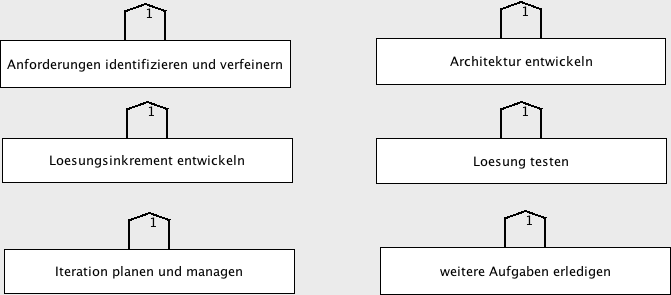
\includegraphics[width=\linewidth]{ElaborationDecUnter} %pdf, jpg, png...
  \caption{Phasen Open UP Unterprozess Elaboration- deklarativ} 
  \label{fig:ElaborationDecUnter}
\end{center}
\end{figure}

Die deklarative Modellierung der Iteration Construction kann Abbildung \ref{fig:ConstructionDecUnter} entnommen werden. Hier werden die sechs Aktivitäten \textit{Anforderungen identifizieren und verfeinern, Lösungsinkrement entwickeln, Lösung testen, Iteration planen und managen, weitere Aufgaben erledigen} und \textit{Produktdokumentation und Training erstellen} nebeneinander parallel ausgeführt.
\begin{figure}[htp]
\begin{center}
  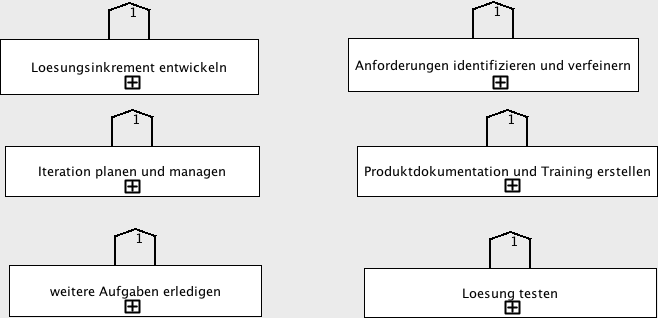
\includegraphics[width=\linewidth]{ConstructionDecUnter} %pdf, jpg, png...
  \caption{Phasen Open UP Unterprozess Construction- deklarativ}
  \label{fig:ConstructionDecUnter}
\end{center}
\end{figure}

In \ref{fig:TransitionDecUnter} ist die deklarative Modellierung der Iteration Transition abgebildet.\newline
Die Aktivitäten \grqq Release vorbereiten, Produkt Training vorbereiten, Lösungsinkrement entwickeln, Lösung testen, Iteration planen und managen, weitere Aufgaben erledigen\grqq \ werden parallel zueinander bearbeitet. Produkt Training durchfuehren sowie \grqq Release für die Produktion freigeben\grqq \  können anschließen parallel zueinander ausgeführt werden. Daher befindet sich zwischen diesen beiden Aktivitäten und allen anderen Aktivitäten das Constraint \textit{precedence}.

\begin{figure}[htp]
\begin{center}
  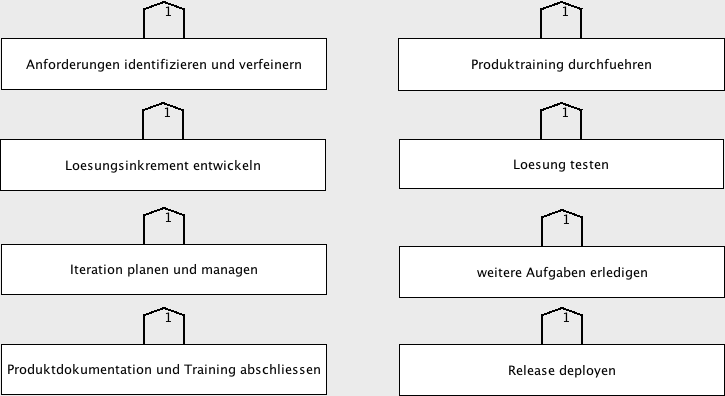
\includegraphics[width=\linewidth]{TransitionDecUnter} %pdf, jpg, png...
  \caption{Phasen Open UP Unterprozess Transition- deklarativ}
  \label{fig:TransitionDecUnter}
\end{center}
\end{figure}



Im weiteren Verlauf wird aus jeder der vier Iterationen Inception, Elaboration, Construction und Transition des Open UP jeweils ein Unterprozess modelliert, da die Abbildung aller Unterprozesse aus jeder Phase den Rahmen der Arbeit sprengen würde. \newline
Somit wird für die Iteration Inception der Unterprozess \textit{Iteration planen und managen}, für die Itertion Elaboration der Unterprozess \textit{Anforderungen identifizieren und verfeinern}, für die Iteration Construction der Unterprozess \textit{Release deployen} und für die Iteration Transition der Unterprozess \textit{Produktdokumentation und Training erstellen} modelliert. Außerdem wird der in den drei Iterationen Elaboration, Construction und Transition wiederkehrende Unterprozess \textit{Lösungsinkrement entwickeln} modelliert.


Die deklarative Modellierung von Lösungsinkrement entwickeln kann Abbildung \ref{fig:Develop} entnommen werden.\newline
Falls eine \grqq Lösung designt\grqq \ wird, muss danach der \grqq Entwicklertest implementiert\grqq \ werden. Dies ist durch das Constraint \textit{chain response} zwischen diesen beiden Aktivitäten verlangt. Wenn der Entwicklertest implementiert wird, muss er danach auch ausgeführt werden und er kann nur ausgeführt werden, falls er vorher implementiert wurde (Constraints \textit{chain response} und \textit{precedence}).\newline
Bevor die Lösung implementiert werden kann, muss vorher der Entwicklertest ausgeführt werden (Constraint \textit{precedence}) und nach der Implementierung der Lösung muss nochmals der Entwicklertest ausgeführt werden (Constraint chain response).\newline
Vor dem \grqq Integrieren\grqq \ muss der Entwicklertest ausgeführt worden sein, was durch das Constraint \textit{precedence} vorgegeben wird.
\begin{figure}[htp]
\begin{center}
  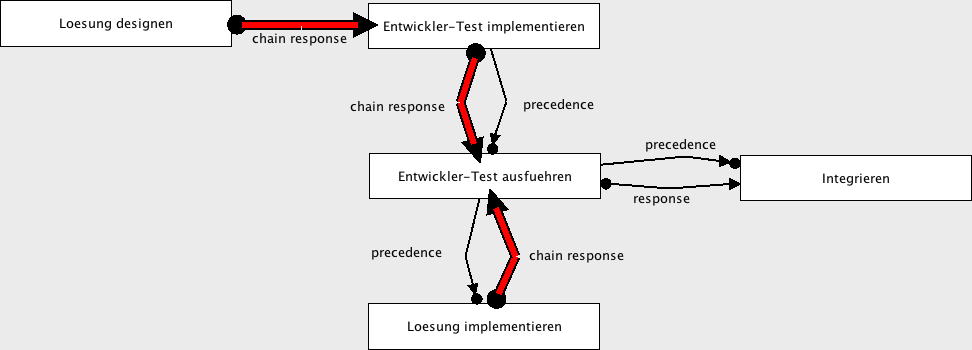
\includegraphics[width=\linewidth]{DevelopSolutionIncrement} %pdf, jpg, png...
  \caption{Lösungsinkrement entwickeln- deklarativ}
  \label{fig:Develop}
\end{center}
\end{figure}

Die deklarative Modellierung von Iteration planen und managen findet sich in den Abbildungen \ref{fig:IterationPlanenDec} und \ref{fig:UmgebungVorbereitenDec}. Gestartet werden kann mit den Aktivitäten \grqq Iteration planen\grqq \ oder \grqq Arbeitsaufgaben aussuchen\grqq, da diese unabhängig voneinander und von zwei verschiedenen Personen ausgeführt werden können.\newline
Danach können entweder die Aktivitäten \grqq Umgebung vorbereiten\grqq \ oder \grqq Arbeitsaufgaben in Entwicklungsaufgaben einteilen\grqq \ ausgeführt werden. Diese sind jeweils mit ihrer Vorgängeraktivität durch das Constraint \textit{succession} verbunden und müssen deshalb auf die Ausführung ihres Vorgängers warten und nach dessen Ausführung bearbeitet werden.\newline
Das gleiche Ausführungsverhalten gilt auch für die anderen Aktivitäten im Prozess. 



\begin{figure}[htp]
\begin{center}
  \includegraphics[width=\linewidth]{IterationPlanenDec} %pdf, jpg, png...
  \caption{Iteration planen und managen-Inception deklarativ}
  \label{fig:IterationPlanenDec}
\end{center}
\end{figure}

\begin{figure}[htp]
\begin{center}
  \includegraphics[width=\linewidth]{UmgebungvorbereitenDec} %pdf, jpg, png...
  \caption{Iteration planen und managen- Inception Unterprozess Umgebung vorbereiten- deklarativ}
  \label{fig:UmgebungVorbereitenDec}
\end{center}
\end{figure}


In Abbildung \ref{fig:IdentifyAndRefineDecKlein} ist die deklarative Modellierung von Anforderungen identifizieren und verfeinern dargestellt.\newline
Zu Beginn muss die Aktivität \grqq Anforderungen identifizieren und abgrenzen\grqq \ ausgeführt werden, was durch das init-Label dargestellt ist. Im Anschluss muss die Aktivität \grqq Use-Case-Szenarien detaillieren\grqq \ ausgeführt werden. Dies ist durch das Constraint \textit{chain response} festgelegt. Das Constraint \textit{precedence} legt hingegen fest, dass bevor \grqq Use-Case-Szenarien detaillieren\grqq \ ausgeführt werden kann, zunächst \grqq Anforderungen identifizieren und abgrenzen\grqq \ bearbeitet werden muss. Die gleichen Constraints gelten zwischen \grqq Use-Case-Szenarien detaillieren\grqq \ und \grqq Systemweite Anforderungen detaillieren\grqq \ sowie zwischen \grqq Systemweite Anforderungen detaillieren\grqq \ und \grqq Testfaelle erstellen\grqq. Alle Aktivitäten werden genau einmal ausgeführt, was jeweils durch das 1-Label dargestellt ist. 

\begin{figure}[h]
\begin{center}
  \includegraphics[width=\linewidth]{IdentifyAndRefineDecKlein} %pdf, jpg, png...
  \caption{Anforderungen identifizieren und verfeinern-Elaboration}
  \label{fig:IdentifyAndRefineDecKlein}
\end{center}
\end{figure}



Abbildung \ref{fig:DevelopProductDecKlein} zeigt die deklarative Modellierung von Produktdokumentation und Training erstellen.
Zu Beginn muss die Aktivität \grqq Produktdokumentation entwickeln\grqq \ ausgeführt werden, was durch das init-Label dargestellt ist. Im Anschluss muss die Aktivität \grqq Benutzerdokumentation entwickeln\grqq \ bearbeitet werden. Dies ist durch das Constraint \textit{chain response} festgelegt. Das Constraint \textit{precedence} legt hingegen fest, dass bevor \grqq Benutzerdokumentation entwickeln\grqq \ ausgeführt werden kann, zunächst \grqq Produktdokumentation entwickeln\grqq \ bearbeitet werden muss. Die gleichen Constraints gelten zwischen \grqq Benutzerdokumentation entwickeln\grqq \ und \grqq Unterstützungsdokumentation entwickeln\grqq \ sowie zwischen \grqq Unterstützungsdokumentation entwickeln\grqq \ und \grqq Trainingsmaterial entwickeln\grqq. Alle Aktivitäten werden genau einmal ausgeführt, was jeweils durch das 1-Label beschriebenist. 

\begin{figure}[htp]
\begin{center}
  \includegraphics[scale=0.6]{DevelopProductDecKlein} %pdf, jpg, png...
  \caption{Produktdokumentation und Training erstellen-Construction}
  \label{fig:DevelopProductDecKlein}
\end{center}
\end{figure}

Abbildung \ref{fig:DeployReleaseDecKlein} zeigt die deklarative Modellierung von Deploy Release.\newline
Zu Beginn muss Die Aktivität\grqq Release zusammenstellen\grqq \ bearbeitet werden, was durch das init-Constraint vorgegeben ist. Danach wird muss die Aktivität \textit{Deploymentplan ausfuehren} durchgeführt werden (Constraint response), aber erst nachdem \grqq Release zusammenstellen\grqq \ durchgeführt wurde (Contsraint precedence).\newline
Die gleichen Constraints gelten zwischen den Aktivitäten \grqq Deploymentplan ausfuehren\grqq \ und \grqq erfolgreiches Deployment sicherstellen\grqq.\newline
Nach Abschluss der Aktivität \grqq erfolgreiches Deployment sicherstellen\grqq \ kann entweder die Aktivität \grqq Backoutplan ausfuehren\grqq \ ausgeführt werden, welche optinal ist (0..1 Constraint) oder die Aktivität \textit{Release-Mitteilungen uebermitteln}, welche auf jeden Fall ausgeführt werden muss.\newline 
Nach Ausführung von \grqq Release-Mitteilungen uebermitteln\grqq \ darf \grqq Backoutplan ausfuehren\grqq \ nicht mehr durchgeführt werden. Dies stellt das Constraint \textit{not succession} sicher.
\begin{figure}[htp]
\begin{center}
  \includegraphics[width=\linewidth]{DeployReleaseDecKlein} %pdf, jpg, png...
  \caption{Release deployen-Transition}
  \label{fig:DeployReleaseDecKlein}
\end{center}
\end{figure}

\clearpage

\subsection{Vergleich}

Nachfolgend wird der vergleich der erstellten Modelle für den Open UP anhand der in Kapitel 4 definierten Anforderungen durchgeführt.

\subsubsection {Phasen Open UP}


Abbildung \ref{fig:PhasenOpenUpExcel} zeigt die Auswertung der Elemente im Modell Phasen des Open UP. Während bei BPMN vier Aktivitäten, acht Gateways (keine unterschiedlichen) und 17 Sequenzflusselemente, also gesamt 29 Elemente für das Modell benötigt werden, werden in ConDec nur vier Aktivitäten und sechs Constraints (zwei verschiedene), also insgesamt zehn Elemente verwendet.

\begin{figure}[htp]
\begin{center}
  \includegraphics[scale=0.6]{PhasenOpenUpExcel} %pdf, jpg, png...
  \caption{Phasen Open UP}
  \label{fig:PhasenOpenUpExcel}
\end{center}
\end{figure}



\subsubsection {Iterationen Open UP-Inception}

Die Anzahl der Elemente zur Darstellung der Iterationen Inception, Elaboration, Construction und Transition in ConDec und BPMN können Abbildung \ref{fig:PhasenExcel} entnommen werden. BPMN benötigt somit insgesamt 19 Elemente zur Darstellung der Iteration Inception (vier Aktivitäten, vier Gateways und 15 Verbindungselemente), ConDec nur zehn (vier Aktivitäten, sechs Constraints). Bei BPMN wird nur eine Sorte an Gateways verwendet und bei ConDec werden zwei unterschiedliche Constraints benötigt.\newline
\begin{figure}[htp]
\begin{center}
  \includegraphics[width=\textwidth]{PhasenExcel} %pdf, jpg, png...
  \caption{Open UP-Inception}
  \label{fig:PhasenExcel}
\end{center}
\end{figure}

Zur Darstellung der Iteration Elaboration bedarf es in BPMN insgesamt 22 Elementen und in ConDec 14 Elementen wie Abbildung \ref{fig:PhasenExcel} entnommen werden kann. Weiterhin werden jeweils sechs Aktivitäten in beiden Prozessmodellierungssprachen verwendet. In BPMN sind zwei Gateways (keine unterschiedlichen) und 14 Sequenzflusselemente, also insgesamt 16 Verbindungselemente notwendig. ConDec hingegen braucht acht Existenz-Constraints. \newline

Abbildung \ref{fig:PhasenExcel} kann die Anzahl der Elemente zur Darstellung der Iteration Construction entnommen werden. Demnach benötigt es in BPMN 24 Elemente und in ConDec 12 Elemente zur Darstellung des Prozesses. Sowohl in BPMN, als auch in ConDec werden jeweils sechs Aktivitäten benötigt. In BPMN sind vier Gateways (keine unterschiedlichen) und 14 Sequenzflusselemente erforderlich. In ConDec werden sechs Existenz-Constraints zur Darstellung des Ablaufes verwendet.\newline


Die Anzahl der notwendigen Elemente zur Darstellung der Iteration Transition kann Abbildung \ref{fig:PhasenExcel} entnommen werden. Somit bedarf es jeweils acht Aktivitäten. BPMN benötigt vier Gateways (keine unterschiedlichen) und 19 Sequenzflusselemente zur korrekten Modellierung. In ConDec braucht es insgesamt acht Existenz-Constraints und 12 Constraints zur Darstellung des Ablaufes.\newline


In Abbildung \ref{fig:LoesungsinkrementExcel} ist die Anzahl der Elemente zur Darstellung des Prozesses Lösungsinkrement entwickeln abgebildet. Es werden sowohl in BPMN, als auch in ConDec jeweils fünf Aktivitäten verwendet. Weiterhin werden in BPMN 15 Sequenzflusselemente und fünf Gateways gebraucht. Dabei handelt es sich ausschließlich um XOR-Gateways. Das mit ConDec erstellte Modell benötigt insgesamt sechs Constraints. Hierbei werden insgesamt drei unterschiedliche Constraints benutzt. Insgesamt werden in BPMN 25 Elemente zum Modellieren eingesetzt und in ConDec 11 Elemente.\newline

\begin{figure}[htp]
\begin{center}
  \includegraphics[scale=0.6]{LoesungsinkrementExcel} %pdf, jpg, png...
  \caption{Lösungsinkrement entwickeln}
  \label{fig:LoesungsinkrementExcel}
\end{center}
\end{figure}


Abbildung \ref{fig:OpenUPExcel} kann die Anzahl der Elemente, welche jeweils zur Darstellung des Unterprozesses Iteration planen und managen notwendig sind, entnommen werden. Sowohl in BPMN, als auch in ConDec werden somit jeweils 11 Aktivitäten benötigt. In BPMN werden keine Gateways und 15 Sequenzflüsse verwendet. In ConDec sind zur korrekten Darstellung 21 Constraints notwendig. Somit werden in BPMN insgesamt 26 Elemente und in ConDec 32 Elemente gebraucht.\newline

\begin{figure}[htp]
\begin{center}
  \includegraphics[width=\textwidth]{OpenUPExcel} %pdf, jpg, png...
  \caption{Open UP-Iteration planen}
  \label{fig:OpenUPExcel}
\end{center}
\end{figure}

In Abbildung \ref{fig:OpenUPExcel} sind die Anzahl der Elemente zur Darstellung von Anforderungen identifizieren und verfeinern abgebildet. Demnach werden sowohl in BPMN, als auch in ConDec jeweils vier Aktivitäten benötigt. Weiterhin sind keine Gateways und 5 Sequenzflusselemente in BPMN zur Darstellung nötig. In ConDec werden drei Constraints verwendet, aber keine unterschiedlichen. Insgesamt werden zur korrekten Abbildung des Metamodells in BPMN neun Elemente und in ConDec 11 Elemente eingesetzt.\newline


Die Anzahl der Elemente zur Darstellung des Prozesses Produktdokumentation entwickeln kann Abbildung \ref{fig:OpenUPExcel} entnommen werden. Es werden somit jeweils vier Aktivitäten zur Darstellung genutzt. Weiterhin werden in BPMN keine Gateways und sieben Sequenzflusselemente gebraucht. In ConDec sind zur Darstellung sieben Constraints notwendig jedoch keine unterschiedlichen Constraints. Insgesamt werden in BPMN neun Elemente und in ConDec 11 Elemente verwendet.\newline


Wie viele Elemente zur Modellierung des Prozesses Release deployen benötigt werden, ist in Abbildung \ref{fig:OpenUPExcel} aufgeführt. Jeweils fünf Aktivitäten werden in BPMN und ConDec eingesetzt. In BPMN sind zwei Gateways (keine verschiedenen) und neun Sequenzflusselemente zur Darstellung des Ablaufes notwendig. In ConDec werden hierfür fünf Constraints (drei unterschiedliche)  und fünf Existenz-Constraints benötigt. Somit sind insgesamt 16 Elemente in BPMN und 15 Elemente in ConDec zur Darstellung notwendig. \newline


Der Grundsatz der syntaktischen \textit{Richtigkeit} kann von beiden Prozessmodellierungssprachen eingehalten werden, denn alle imperativen und deklarativen Modelle lassen sich unter Einhaltung der Notationsregeln der jeweiligen Modellierungssprachen erstellen [A 1.1].\newline
Bei dem Grundsatz der semantischen \textit{Richtigkeit} [A 1.2] tritt bei ConDec wiederum das Problem auf, dass Rollen und Artefakte nicht darstellbar sind. Zwar ist dies bei den Phasen des Open UP kein Problem, da hier noch keine Rollen und Artefakte zugeordnet werden, jedoch bei den anderen Prozessen des Open UP (Iteration planen und managen, Anforderungen identifizieren und verfeinern, Produktdokumentation entwickeln und Release deployen). Da hier keine Rollen visualisierbar sind, kann das jeweils im Metamodell enthaltene Verhalten in den ConDec-Modellen nicht vollständig wiedergegeben werden. Hierdurch leidet der Nutzen des Metamodells. \newline
Somit ist BPMN in Bezug auf die \textit{Richtigkeit} die geeignetere Modellierungssprache, da sie beide Anforderungen ([A 1.1] und [A 1.2]) erfüllt und ConDec nur [A 1.1] erfüllt.\newline

Der Grundsatz des \textit{systematischen Aufbaus} [A 2.1] kann wiederum nur von BPMN eingehalten werden, da ConDec keine Möglichkeit bietet, Artefakte im Prozessmodell selbst zu visualisieren.\newline
Auch hier weist BPMN eine bessere Eignung zur Modellierung auf.\newline

Die \textit{Relevanz} [A 3.1] lässt sich nur bei BPMN einhalten, denn es ist wieder bei den in ConDec erstellten Modellen nicht möglich, Rollen und Artefakte zu visualisieren und somit können nicht alle minimal relevanten Informationen im ConDec Modell abgebildet werden..\newline

In Bezug auf die \textit{Klarheit} fällt gerade bei Betrachtung der Modelle der Iterationen Inception, Elaboration, Construction und Transition auf, das bei Modellen, bei denen mehrere Aktivitäten einfach parallel zueinander ablaufen, in BPMN deutlich mehr Sequenzflusselemente zur Darstellung des gleichen Sachverhaltes notwendig sind als Existenz Constraints in ConDec. Zudem werden bei BPMN auch noch jeweils zwei Gateways benötigt. Somit weist BPMN sowohl bei dem einfach gewichteten Punkt Sequenzfluss/Existenz Constraints, als auch bei den doppelt gewichteten punkten Gateways/Constraints und unterschiedliche Gateways/Constraints eine höhere Anzahl auf als ConDec und bringt somit bei diesen drei Modellen komplexere Modelle hervor [A 4.1]. \newline
Bei der Iteration Transition hingegen weist BPMN nur bei dem einfach gewichteten Punkt Sequenzfluss/Existenz einen höheren Wert auf. Beim doppelt gewichteten punkt Gateways/Constraints weist das ConDec Modell eine deutlich höhere Anzahl auf. Somit ist hier insgesamt das mit ConDec erstellte Modell leicht komplexer als das BPMN-Modell [A 4.1].\newline
Zur Darstellung der  \grqq Phasen des Open UP \grqq \ wird für den Prozess in BPMN beim einfach gewichteten Punkt Sequenzfluss/Existenz eine höhere Anzahl an Sequenzflusselementen benötigt als Existenz Constraints bei ConDec. Ebenso werden bei dem doppelt gewichteten Punkt Gateways/Constraints bei BPMN mehr Elemente verwendet. Beim ebenfalls doppelt gewichteten Punkt unterschiedliche Gateways/Constraints werden bei ConDec mehr Elemente eingesetzt. Somit ist insgesamt das mit BPMN erstellte Modell das leicht komplexere [A 4.1].  \newline
Beim Prozess \grqq Lösungsinkrement entwickeln \grqq \ werden fünf Gateways in BPMN verwendet und bei ConDec werden sechs Constraints benötigt. Bei ConDec werden drei verschiedene Constraints verwendet, bei BPMN jedoch keine verschiedenen Gateways, sondern immer nur das XOR- Gateway. Somit weist BPMN beim einfach gewichteten Punkt Sequenzfluss/Existenz eine höhere Anzahl auf. Bei den doppelt gewichteten Punkten Gateways/Constraints und unterschiedliche Gateways/Constraints weist ConDec eine höhere Anzahl auf. Dadurch ist in Anbetracht von [A 4.1] das ConDec Modell das komplexere.\newline
Im BPMN Modell ist der Startpunkt durch das Startzeichen gekennzeichnet. Beim ConDec Modell kann kein eindeutiger Start im Modell angegeben werden, da mehrere Aktivitäten als Start infrage kommen [A 4.2]. Dies erhöht die Komplexität des ConDec Modells ebenfalls, da die Aktivitäten, mit welchen gestartet werden kann nicht auf einen Blick erkennbar sind. \newline
Daher kann zusammenfassend gesagt werden, dass die Komplexität des ConDec Modells leicht höher ist, da dies sowohl bei [A 4.1], als auch bei [A 4.2] der Fall ist.\newline
Im Prozess  \grqq Iteration planen und managen\grqq \ gibt es keine Verzweigungen. In ConDec werden sieben Constraints zur Darstellung verwendet. Beim einfach gewichteten Punkt Sequenzfluss/Existenz hat BPMN eine höhere Anzahl. Bei den doppelt gewichteten Punkten Gateways/Constraints und unterschiedliche Gateways/Constraints weist ConDec eine höhere Anzahl auf.\newline
Bei den Prozessen  \grqq Anforderungen identifizieren und verfeinern \grqq \ und  \grqq Produktdokumentation entwickeln \grqq \ weisen die ConDec-Modelle jeweils drei Constraints auf und die BPMN-Modelle keine Gateways. Damit weist BPMN wiederum beim einfach gewichteten Punkt Sequenzfluss/Existenz einen höheren Wert auf und ConDec bei den doppelt gewichteten Punkten Gateways/Constraints und unterschiedliche Gateways/Constraints. Somit ist nach [A 4.1] das BPMN-Modell das weniger komplexe.\newline
Beim Prozess Release deployen werden in ConDec insgesamt fünf Constraints (drei verschiedene) zur Darstellung des Sachverhaltes benötigt, in BPMN nur zwei Gateways. Somit liegt hier das BPMN-Modell in Bezug auf die Komplexität unter dem ConDec-Modell und ist somit das verständlichere, da es bei den doppelt gewichteten Punkten Gateways/Constraints und unterschiedliche Gateways/Constraints eine geringere Anzahl aufweist [A 4.1].\newline
Somit liegt ConDec bei der Darstellung der Phasen, in denen viele parallele Abläufe dargestellt werden bei der \textit{Klarheit} vorne, während bei den anderen Modellen, bei denen es Schleifen oder Abläufe ohne Verzweigungen zum Darstellen gibt, BPMN vorne liegt.\newline

Die \textit{Wirtschaftlichkeit} lässt sich auch beim Open UP bei den Prozessmodellen Inception, Elaboration, Construction sowie bei den Phasen des Open UP mit ConDec besser einhalten, als mit BPMN.  \newline
Bei den anderen Modellen des Open UP jedoch gibt es bei den mit ConDec erstellten Modellen deutlich mehr Constraints und auch unterschiedliche Constraints, als  Gateways bei BPMN. Aus diesem Grund sind hier genau gegensätzlich die ConDec- Modelle komplexer und benötigen somit einen höheren geistigen Aufwand zum Erstellen. \newline
Hierfür gelten die gleichen Argumente wie soeben bei \textit{Klarheit, [A 4.1]} beschrieben [A 5.1]
Somit können hier einerseits mit ConDec bei der Darstellung der Phasen des Open UP und andererseits bei den anderen Modellen des Open UP die BPMN-Modelle die \textit{Wirtschaftlichkeit} besser erfüllen. Somit kann hier keine der beiden Sprachen als grundsätzlich geeigneter angesehen werden.\newline


Die Abläufe der Diagramme wurden in Signavio und Declare getestet und dadurch ist hier ihre \textit{Vergleichbarkeit} gewährleistet [A 6.1].\newline
Bei der Darstellung der Phasen des Open UP werden doppelt so viele Elemente in ConDec, wie in BPMN verwendet. Hier ist deshalb die \textit{Vergleichbarkeit} nicht ganz gewährleistet. Bei den anderen Modellen des Open UP unterscheidet sich die Anzahl der Elemente kaum voneinander, wodurch die Vergleichbarkeit hier gewährleistet ist [A 6.2]. \newline
Bei ConDec muss wieder auf die Darstellung von Artefakten und Rollen verzichtet werden, wodurch die \textit{Vergleichbarkeit} der Modelle von ConDec behindert wird. Somit weisen hier beide Prozessmodellierungssprachen Stärken und Schwächen auf [A 6.3].\newline

Eine Zusammenfassung, welche Modellierungssprache bei welchem Grundsatz eher überzeugt hat, kann Abbildung \ref{fig:TabelleOpenUP} entnommen werden. \newline


\begin{figure}[htp]
\begin{center}
  \includegraphics[scale=0.6]{TabelleOpenUP} %pdf, jpg, png...
  \caption{Übersicht Vergleich Open UP}
  \label{fig:TabelleOpenUP}
\end{center}
\end{figure}


\section{V-Modell XT}


Das V-Modell XT zählt zu den schwergewichtigen Prozessmodellen \cite{Hanser2010}. Es wird als Entwicklungsstandard für die Durchführung von IT-Vorhaben in der öffentlichen Verwaltung in Deutschland herangezogen \cite{Kuhrmann2011}. Beschrieben werden im V-Modell XT die Abläufe im Verlauf eines Entwicklungsprojektes über Produkte, Rollen und Aktivitäten \cite{Friedrich2008}. Es wird somit ganz genau geregelt, \textit{Wer}, \textit{Wann}, \textit{Was} in einem Projekt zu tun hat \cite{2004vmodell}. Vorgehensbausteine ermöglichen neben einer Modularisierung der Abläufe auch eine flexible Zusammenstellung, wodurch das V-Modell XT auf die jeweils eigene Situation angepasst werden kann. \cite{Friedrich2008,Zoerner2012}. \newline

\subsection{Analyse V-Modell XT}

Abbildung \ref{fig:grundstruktur} zeigt die Grundstruktur des V-Modell XT, welche im Folgenden detailliert erläutert wird.
\begin{figure}[htp]
\begin{center}
  \includegraphics[width=\linewidth]{grundstruktur} %pdf, jpg, png...
  \caption{Grundstruktur V-Modell XT nach \cite{2004vmodell}}
  \label{fig:grundstruktur}
\end{center}
\end{figure}

\subsubsection{Projekttypen}
Nicht alle V-Modell-Projekttypen laufen nach exakt demselben Schema ab. Auf Grund ihrer charakteristischen Eigenschaften lassen sie sich demnach in unterschiedliche Projekttypen einteilen. Abbildung \ref{fig:Projekttypen} gibt einen ersten Überblick über die verschiedenen Projekttypen im V-Modell XT \cite{2004vmodell}.

\begin{figure}[htp]
\begin{center}
  \includegraphics[width=\linewidth]{v-modell-rollen} %pdf, jpg, png...
  \caption{Projekttypen V-Modell XT nach \cite{2004vmodell}}
  \label{fig:Projekttypen}
\end{center}
\end{figure}

Es existieren somit vier verschiedene Projekttypen: \grqq Systementwicklungsprojekt eines Auftraggebers\grqq, \grqq Systementwicklungsprojekt eines Auftragnehmers\grqq, \grqq Systementwicklungsprojekt eines Auftraggebers/Auftragnehmers\grqq \ und \grqq Einführung und Pflege eines organisationsspezifischen Vorgehensmodells\grqq \ \cite{reinhard2008}. \newline

Es werden drei verschiedene Projektrollen unterschieden, welche dem jeweiligen Projekttyp entsprechen: In der Rolle \textit{Auftragnehmer} wird ein vom \textit{Auftraggeber} spezifiziertes System entwickelt. Die Systementwicklung wird an einen oder mehrere \textit{Arbeitnehmer} weiter gegeben, wenn man sich in der Rolle \textit{Arbeitgeber} befindet. Das System  wird selbst entwickelt in der Rolle \grqq Auftraggeber/Auftragnehmer\grqq \ \cite{brack2010,2004vmodell}.\newline


Beim \grqq Systementwicklungsprojekt eines Auftraggebers\grqq \ wird die Entwicklung des Projektgegenstandes im Projektverlauf  ausgeschrieben und der Auftragnehmer trifft eine Auswahl anhand der eingehenden Angebote. Der Auftragnehmer, welcher für die Entwicklung des Projektgegenstandes ausgewählt wurde, entwickelt den Projektgegenstand, welcher dann vom Auftragnehmer abgenommen wird \cite{reinhard2008,2004vmodell}.\newline
Umgekehrt wird beim \grqq Systementwicklungsprojekt eines Auftragnehmers\grqq \ im Laufe des Projektes ein Angebot erstellt und bei Auswahl durch den Auftraggeber ein Projektgegenstand entwickelt, welcher abschließend an den Auftraggeber ausgeliefert und von diesem abgenommen wird \cite{reinhard2008,2004vmodell}.\newline
Bei \grqq Einführung und Pflege eines organisationsspezifischen Vorgehensmodells\grqq \ geht es um Projekte, welche Prozessmodelle z.B. das V-Modell einführen und verbessern wollen. Für diesen Zweck ist eine Analyse des vorherigen Prozessmodelles notwendig und etwaige Verbesserungsmöglichkeiten sind zu erfassen und durchzuführen \cite{reinhard2008,2004vmodell}.\newline
Wie aus Abbildung \ref{fig:Projekttypen} ersichtlich ist, kann es sich im V-Modell XT beim Projektgegenstand um ein Hardware (HW)-System, ein Software (SW)-System, ein eingebettetes System oder eine Systemintegration handeln \cite{brack2010,2004vmodell}. \newline

\subsubsection{Projekttypvarianten}
Für jeden der Projekttypen, gibt es im V-Modell XT mindestens eine passende Projekttypvariante. Diese bestimmt die Rahmenbedingungen für mögliche Abläufe eines Projektes. In Abbildung \ref{fig:Projekttypvarianten} sind die verschiedenen Projekttypvarianten des V-Modell XT aufgelistet und es wird gezeigt, mit welchen Merkmalen die zugehörigen Projekttypvarianten ausgewählt werden können \cite{2004vmodell}.   
\begin{figure}[htp]
\begin{center}
  \includegraphics[width=\linewidth]{Projekttypvarianten-v-modell} %pdf, jpg, png...
  \caption{Zuordnung der Projekttypvarianten zu den Projekttypen des V-Modell XT \cite{2004vmodell}}
  \label{fig:Projekttypvarianten}
\end{center}
\end{figure}

Für den Projekttyp \grqq Systementwicklungsprojekt (AG)\grqq \ existieren zwei verschiedene Projekttypvarianten, welche je nach \grqq Auftragsstruktur\grqq \ ausgewählt werden. Falls der Auftraggeber mit nur einem Auftragnehmer zusammen arbeitet, ergibt sich die Projekttypvariante \grqq Systementwicklungsprojekt (AG)- Projekt mit einem Auftragnehmer\grqq. Arbeitet der Auftraggeber mit mehreren Auftragnehmern zusammen, ergibt sich die Projekttypvariante \grqq Systementwicklungsprojekt (AG)- Projekt mit mehreren Auftragnehmern\grqq \ \cite{2004vmodell}.\newline
Bei den Projekttypen \grqq Systementwicklungsprojekt (AN)\grqq \ und \grqq Systementwicklungsprojekt (AG/AN)\grqq \ wird die Unterscheidung anhand des Systemlebenszyklusausschnitt des Projektes durchgeführt. Somit wird in den Systemlebenszyklusausschnitten Entwicklung, Weiterentwicklung und Migration eine andere Projekttypvariante gewählt als in Wartung und Pflege \cite{2004vmodell}.\newline 
Für den Projekttyp \grqq Einführung und Pflege eines organisationsspezifischen Vorgehensmodells\grqq \ existiert nur eine einzige Projekttypvariante, weshalb hier keine weiteren Merkmale zur Bestimmung der Projekttypvariante notwendig sind \cite{2004vmodell}.\newline

  
 \subsubsection{Vorgehensbausteine}
Modulare, aufeinander aufbauende Vorgehensbausteine, bilden den Kern des V-Modell XT. Vorgehensbausteine sind selbständig entwickelbare und änderbare Einheiten und bestehen aus Aktivitäten, Produkten und Rollen. Sie geben einerseits vor, \grqq Was\grqq{}  in einem Projekt zu tun ist, also welche Produkte zu erstellen sind und andererseits \grqq Wer\grqq, also welche konkrete Rolle für das jeweilige Produkt verantwortlich ist. Abbildung \ref{fig:vorgehensbausteine} gibt einen Überblick über diese \cite{ruf2008, 2004vmodell}.\newline

\begin{figure}[htp]
\begin{center}
  \includegraphics[width=\linewidth]{vorgehensbaustein} %pdf, jpg, png...
  \caption{Vorgehensbausteine V-Modell XT nach \cite{2004vmodell}}
  \label{fig:vorgehensbausteine}
\end{center}
\end{figure}

Ergebnisse und Zwischenergebnisse werden Produkte genannt. Komplexe Produkte können in ein oder mehrere Themen gegliedert werden und inhaltlich zusammengehörende Produkte können zu einer Disziplin zusammengefasst werden. Produkte können hierbei auch voneinander abhängig sein, sowohl innerhalb eines Vorgehensbausteins, als auch zwischen verschiedenen Vorgehensbausteinen \cite{2004vmodell}.\newline
Jedes Produkt wird von genau einer Aktivität fertig gestellt. Aktivitäten legen auch fest, wie die einzelnen Produkte zu bearbeiten sind. Sie bestehen aus einer oder mehreren Teilaktivitäten, sogenannten Arbeitsschritten. Diese stellen eine Art Arbeitsanleitung dar und bearbeiten eine oder mehrere Themen \cite{2004vmodell}.\newline
Durch Rollen werden eine Menge von Aufgaben und Verantwortlichkeiten gekapselt, wodurch das V-Modell XT unabhängig von organisatorischen Rahmenbedingungen bleibt. Eine Zuordnung von Personen bzw. Organisationseinheiten zu einer Rolle erfolgt erst zu Beginn eines Projektes. Es wird jedem Produkt genau eine Rolle als Verantwortlicher zugewiesen. Weitere Rollen können am Produkt als Mitwirkende mitarbeiten \cite{2004vmodell}. \newline



\subsubsection{V-Modell XT-Kern und Vorgehensbausteinlandkarte}

Um ein spezifisches Projekt an ein V-Modell XT-Projekt anzupassen, ist für jeden Projekttyp und jede Projekttypvariante genau vorgegeben, welche Vorgehensbausteine jeweils anzuwenden sind \cite{2004vmodell}. Hierdurch kann also ein individuelles V-Modell für ein Projekt erstellt werden \cite{heinrich2007}. Hierfür ist es notwendig, die Vorgehensbausteine für ein V-Modell-Projekt nach den Vorgaben des Projekttyps auszuwählen und festzulegen \cite{2004vmodell}. \newline

\begin{figure}[htp]
\begin{center}
  \includegraphics[width=\linewidth]{landkarte} %pdf, jpg, png...
  \caption{V-Modell XT-Kern und Vorgehensbausteinlandkarte nach \cite{2004vmodell}}
  \label{fig:landkarte}
\end{center}
\end{figure}

 Wie Abbildung \ref{fig:landkarte} zeigt, können die Vorgehensbausteine in die vier Bereiche \grqq Alle V-Modell XT-Projekte\grqq, \grqq Organisationsspezifisches Vorgehensmodell, \grqq AG/AN-Schnittstelle und \grqq Systementwicklung\grqq \  eingeteilt werden \cite{2004vmodell}.\newline
 Im Bereich \grqq Alle V-Modell XT-Projekte\grqq \ finden sich diejenigen Vorgehensbausteine, welche in jedem V-Modell-Projekt herangezogen werden können. Zudem gibt es den V-Modell XT-Kern, in welchem sich die Vorgehensmodelle finden, die in jedem V-Modell-Projekt unerlässlich sind: \grqq Projektmanagement\grqq, \grqq Konfigurationsmanagement\grqq, \grqq Problem- und Änderungsmanagement\grqq \ und \grqq Qualitätssicherung\grqq. Zusätzlich zu diesen verpflichtenden Vorgehensbausteinen können in jedem Projekt noch \grqq Kaufmännisches Projektmanagement\grqq, welches bei der Integration des Projektmanagements in das kaufmännische Management hilft und \grqq Messung und Analyse\grqq, welches Verfahren für die organisationsweite und projektübergreifende Erfassung und Auswertung von Kennzahlen bereitstellt, verwendet werden \cite{2004vmodell}.\newline
 Ist der Zweck eines Projektes die Entwicklung eines \grqq Organisationsspezifischen Vorgehensmodells\grqq, so muss der Vorgehensbaustein \grqq Einführung und Pflege eines organisationsspezifischen Vorgehensmodells\grqq \ hinzugenommen werden. In diesem finden sich Verfahren und Richtlinien für die Einführung eines Vorgehensmodells innerhalb einer Organisation sowie die damit einhergehende Etablierung eines stetigen Verbesserungsprozesses \cite{2004vmodell}.\newline
 Wenn ein Projekt die Entwicklung eines Systems zum Ziel hat, so wird der Bereich \textit{Systementwicklung} herangezogen. In diesem befinden sich die Vorgehensbausteine \grqq Anforderungsfestlegung\grqq, \grqq Systemerstellung\grqq, \grqq HW-Entwicklung\grqq, \grqq SW-Entwicklung\grqq, \grqq Logistikkonzeption\grqq, \grqq Weiterentwicklung und Migration von Altsystemen\grqq, \grqq Evaluierung von Fertigprodukten\grqq, \grqq Benutzbarkeit und Ergonomie\grqq, \grqq Sicherheit\grqq \ sowie \grqq Sicherheit (AN)\grqq \ und \grqq Multi-Projektmanagement\grqq \ \cite{2004vmodell}. \newline
 Im Bereich \grqq AG/AN-Schnittstelle\grqq \ befinden sich die Vorgehensbausteine für die Kommunikation zwischen Arbeitgeber und Arbeitnehmer: \grqq Lieferung und Abnahme (AG)\grqq, \grqq Lieferung und Abnahme (AN)\grqq, \grqq Vertragsschluss (AG)\grqq \ und \grqq Vertragsschluss (AN)\grqq. Hier finden sich Regelungen über den Vertrag zwischen Arbeitgeber und Arbeitnehmer sowie über Lieferung und Abnahme des Entwicklungsgegenstandes \cite{2004vmodell}. \newline
 
 \subsubsection{Projektdurchführungsstrategie}
 Die Vorgehensbausteine im V-Modell XT geben zwar an, welche Produkte jeweils zu erstellen und welche Aktivitäten durchzuführen sind, sie geben jedoch hierbei nicht vor, in welcher Reihenfolge dies geschehen soll. Damit das Projekt trotzdem geplant und gesteuert werden kann, gibt es im V-Modell eine Projektdurchführungsstrategie welche auf den jeweiligen Projekttyp und die Projekttypvariante abgestimmt ist. Hier wird somit die Reihenfolge der Produkte und Aktivitäten festgelegt, also das  \grqq Wann\grqq {} festgelegt. Außerdem werden hier zu erreichende Projektfortschrittsstufen vorgegeben \cite{2004vmodell}. \newline
 
 \subsubsection{Entscheidungspunkte}
Abbildung \ref{fig:entscheidungspunkte} zeigt, dass die in der Projektdurchführungsstrategie vorgegebenen Projektfortschrittsstufen bei Erreichen durch Entscheidungspunkte markiert werden. Diese stellen einen Meilenstein im Projektablauf dar. Um den Entscheidungspunkt zu erreichen, muss eine vorgegebene Menge an Produkten fertig gestellt werden. Hier entscheidet das Projektmanagement über das Erreichen der Projektfortschrittsstufe und das Freigeben des nächsten Projektabschnitts. Die Entscheidungspunkte, welche im V-Modell XT erreicht werden müssen können Abbildung \ref{fig:v-modell} entnommen werden. Diese werden wie im V-Modell XT-Kern in die vier Bereiche \grqq Alle V-Modell-Projekte\grqq, \grqq Organisationsspezifisches Vorgehensmodell\grqq, \grqq AG/AN-Schnittstelle\grqq \ und \grqq Systementwicklung\grqq \ unterschieden \cite{2004vmodell}. \newline
Demnach gelten die Entscheidungspunkte \grqq Projekt genehmigt\grqq, \grqq Projekt definiert, \grqq Iteration geplant\grqq \ und \grqq Projekt abgeschlossen\grqq \ für alle Projekttypen und Projektdurchführungsstrategien \cite{2004vmodell}. \newline
Bei der Systementwicklung werden die Entscheidungspunkte \grqq Anforderungen festgelegt\grqq, \grqq System spezifiziert\grqq, \grqq System entworfen\grqq, \grqq Feinentwurf abgeschlossen\grqq, \grqq Systemelemente realisiert\grqq \ und \grqq System integriert\grqq \ verwendet. Falls das Projekt vor der Anforderungserhebung in mehrere Teilmodelle aufgeteilt werden soll, werden zusätzlich die Entscheidungspunkte \grqq Gesamtprojekt aufgeteilt\grqq \ und \grqq Gesamtprojektfortschritt überprüft\grqq \ hinzugenommen \cite{2004vmodell}. \newline
Die Entscheidungspunkte für die Arbeitgeber/Arbeitnehmer Schnittstelle setzen sich aus \grqq Projekt ausgeschrieben\grqq, \grqq Angebot abgegeben\grqq, \grqq Projekt beauftragt\grqq, \grqq Lieferung durchgeführt\grqq, \grqq Abnahme erfolgt\grqq \ und \grqq Projektfortschritt überprüft\grqq \ zusammen \cite{2004vmodell}. \newline
 Bei der Entwicklung eines organisationsspezifischen Vorgehensmodells kommen die Entscheidungspunkte \grqq Vorgehensmodell analysiert\grqq, \grqq Verbesserung Vorgehensmodell konzipiert\grqq \ und \grqq Verbesserung Vorgehensmodell realisiert\grqq \ zum Einsatz \cite{2004vmodell}. \newline
 Die Entscheidungspunkte legen das \grqq Wann\grqq {} und \grqq Was\grqq {} fest, d.h. wann welche Produkte fertig gestellt sein müssen.

 
 
 \begin{figure}[!htbp]
\begin{center}
  \includegraphics[width=\linewidth]{Entscheidungspunkte} %pdf, jpg, png...
  \caption{Entscheidungspunkte V-Modell XT nach \cite{2004vmodell}}
  \label{fig:entscheidungspunkte}
\end{center}
\end{figure}
 
\begin{sidewaysfigure}[!htbp]
\begin{center}
  \includegraphics[width=\linewidth]{v-modell} %pdf, jpg, png...
  \caption{Entscheidungspunkte für die Projektdurchführungsstrategie nach \cite{2004vmodell}}
  \label{fig:v-modell}
\end{center}
\end{sidewaysfigure}


\clearpage

\subsection{Imperative Modellierung V-Modell XT}

Im Folgenden werden Teile des V-Modells XT modelliert da das ganze V-Modell XT den Rahmen dieser Arbeit sprengen würde. Aus diesem Grund wird zum Einen das \grqq Systementwicklungsprojekt AG/AN\grqq \ ausgewählt. Weiterhin wird ein hierzu gehöriger Unterprozess \grqq Inkrementelle Entwicklung\grqq \ und die hierzu gehörenden Unterprozesse \grqq System entwerfen\grqq \ und \grqq System spezifizieren\grqq \ modelliert.

\subsubsection{Systementwicklungsprojekt AG/AN}


Die imperative Modellierung des Prozesses \grqq Systementwicklungsprojekt AG/AN\grqq \ zeigt Abbildung \ref{fig:Systementwicklungimp}. \newline
Zunächst muss ein Projekt genehmigt und definiert werden. Dies ist durch die einander folgenden Aktivitäten \grqq Projekt genehmigen\grqq \ und \textit{Projekt definieren} dargestellt.\newline
In der nachfolgenden Aktivität müssen sodann die \grqq Anforderungen festgelegt werden\grqq, bevor die \grqq Iteration geplant\grqq \ werden kann. \newline
Hiernach muss entschieden werden, ob eine \grqq Prototypische Entwicklung durchgeführt\grqq, eine \grqq Komponentenbasierte Entwicklung durchgeführt\grqq \ oder eine \grqq Inkrementelle Entwicklung durchgeführt\grqq \ werden soll. Dies wird durch das XOR-Gateway beschrieben, welches nur eine Alternative zulässt.\newline
Anschließend wird das \grqq System abgenommen\grqq. An dieser Stelle wird entschieden, ob erneut zu \grqq Anforderungen festlegen\grqq \ zurückgekehrt wird und der Prozess ab dieser Aktivität erneut startet oder ob zu \grqq Projekt ausschreiben\grqq \ zurückgekehrt wird und der Prozess ab hier erneut startet. Ansonsten endet der Prozess mit der Aktivität \grqq Projekt abschließen\grqq.

\begin{figure}[!htbp]
\begin{center}
  \includegraphics[width=\linewidth]{Systementwicklungimp} %pdf, jpg, png...
  \caption{Systementwicklungsprojekt AG/AN  V-Modell - imperativ}
  \label{fig:Systementwicklungimp}
\end{center}
\end{figure}




\subsubsection{Inkrementelle Entwicklung durchführen}
In Abbildung \ref{fig:Inkrementell} ist die imperative Modellierung des Unterprozesses \grqq Inkrementelle Entwicklung durchführen\grqq \ abgebildet. \newline
Zu Beginn muss das \grqq System spezifiziert\grqq \ werden und anschließend wird es entworfen. \newline
Hiernach wird der \grqq Feinentwurf entworfen\grqq \ und es werden die \grqq Systemelemente realisiert\grqq. Diese beiden Aktivitäten können so oft wie nötig durchgeführt werden, was durch das XOR-Gateway beschrieben ist.  \newline
Im nächsten Schritt wird das \grqq System integriert\grqq \ und es beginnt eine neue Iteration bei der Aktivität System entwerfen.\newline
Falls keine weitere Iteration mehr notwedig ist, wird die \grqq Lieferung durchgeführt\grqq \ und der Unterprozess endet hier. \newline

\begin{figure}[!htbp]
\begin{center}
  \includegraphics[width=\linewidth]{Inkrementell} %pdf, jpg, png...
  \caption{Unterprozess Inkrementelle Entwicklung durchführen V-Modell - imperativ}
  \label{fig:Inkrementell}
\end{center}
\end{figure}



\clearpage


\subsubsection{System entwerfen}

Abbildung \ref{fig:SystementwurfKlein} zeigt die imperative Modellierung des Unterprozesses \grqq System entwerfen\grqq.\newline
Die Aktivitäten \grqq Systemarchitektur erstellen, Unterstütungssystemarchitektur erstellen, Styleguide für die Mensch-Maschine-Schnittstelle erstellen, HW-Architektur erstellen, SW-Architektur erstellen, Datenbankentwurf erstellen, Implementierungs-, Integrations- und Prüfkonzept Unterstützungssystem erstellen, Integrations- und Prüfkonzept Hardware (HW) erstellen, Integrations- und Prüfkonzept Software (SW) erstellen\grqq \ und \grqq Migrationskonzept erstellen\grqq \ werden hier nacheinander ausgeführt.
\begin{sidewaysfigure}[!htbp]
\begin{center}
  \includegraphics[width=\linewidth]{SystementwurfKlein} %pdf, jpg, png...
  \caption{System entwerfen V-Modell - imperativ}
  \label{fig:SystementwurfKlein}
\end{center}
\end{sidewaysfigure}


\subsubsection{System spezifizieren}

Zu Beginn des Unterprozesses \grqq System spezifizieren\grqq \  (Abbildung \ref{fig:BerichtswesenimpKlein}) muss eine \grqq Besprechung durchgeführt\grqq \  werden. Hieraus entsteht das Artefakt \grqq Besprechungsdokument\grqq.\newline
Parallel zu allen anderen Aktivitäten ist bei Bedarf bei jeder Änderung das \grqq Projekttagebuch zu führen\grqq. Dies wird durch das Parallel-Gateway sichergstellt und das XOR-Gateway stellt sicher, dass die Akrtivität so oft durchgeführt wird, wie Anpassungen notwendig sind. \newline
Im nächsten Schritt werden die \grqq Messdaten erfasst\grqq.
In der nachfolgenden Aktivität wird die \grqq Metrik berechnet und ausgewertet\grqq, woraus das Artefakt \grqq Metrikauswertung\grqq \  entsteht.
Anschließend erfolgt die Durchführung der Aktivität \grqq Kaufmännischen Projektstausbericht erstellen\grqq, wobei das Artefakt \grqq {Kaufmännischer Projektstausbericht\grqq \  als Artefakt herauskommt.\newline
Bei der nächsten Aktivität wird der \grqq Projektstatusbericht erstellt\grqq \  und danach wird der \grqq Gesamtprojektfortschritt ermittelt\grqq.\newline
Die Aktivität \grqq QS-Bericht erstellen\grqq \  bringt dann das Artefakt \grqq QS-Bericht hervor\grqq \  und die nachfolgende Aktivität \grqq Projekt abschließen\grqq \  den \grqq Projektabschlußbericht\grqq.

\begin{sidewaysfigure}[!htp]
\begin{center}
  \includegraphics[width=\linewidth]{BerichtswesenimpKlein} %pdf, jpg, png...
  \caption{System spezifizieren-imperativ}
  \label{fig:BerichtswesenimpKlein}
  \end{center}
\end{sidewaysfigure}

\clearpage
\subsection{Deklarative Modellierung V-Modell XT}

Nachfolgend werden die entsprechenden deklarativen Modelle zu den imperativen Modellen modelliert.

\subsubsection{Systementwicklungsprojekt AG/AN}

Die deklarative Modellierung von \grqq Systementwicklungsprojekt AG/AN\grqq  zeigt Abbildung \ref{fig:SystemV}. \newline
Zunächst muss ein Projekt genehmigt und definiert werden. Dies ist durch die aufeinander folgenden Aktivitäten \grqq Projekt genehmigen\grqq \ und \grqq Projekt definieren\grqq \ dargestellt, welche durch das Constraint \textit{succession} verbunden sind.\newline
In der nachfolgenden Aktivität müssen sodann die \grqq Anforderungen festgelegt werden\grqq, bevor die \grqq Iteration geplant\grqq \ werden kann. \newline
Hiernach muss entschieden werden, ob eine \textit{Prototypische Entwicklung durchgeführt}, eine \textit{Komponentenbasierte Entwicklung durchgeführt} oder eine \grqq Inkrementelle Entwicklung durchgeführt\grqq \ werden soll. Dies wird hier durch den Unterprozess \grqq Entwicklung durchführen\grqq \ (Abbildung \ref{fig:SystemVUnter}) dargestellt, da dieser Sachverhalt auf Grund der Schleifen im Prozess ohne Unterprozess nicht darstellbar war. Im Unterprozess kann dann eine der drei Aktivitäten ausgeführt werden, was das Constraint \textit{1of 3} vorgibt.\newline
Anschließend wird das \grqq System abgenommen\grqq.
An dieser Stelle wird enschieden, ob erneut zu \grqq Anforderungen festlegen\grqq \ zurückgekehrt wird und der Prozess ab dieser Aktivität erneut startet oder ob zu \grqq Projekt ausschreiben\grqq \ zurückgekehrt wird und der Prozess ab hier erneut startet. Ansonsten endet der Prozess mit der Aktivität \grqq Projekt abschließen\grqq.

\begin{figure}[!htbp]
\begin{center}
  \includegraphics[width=\linewidth]{SystemV} %pdf, jpg, png...
  \caption{Systementwicklungsprojekt AG/AN  V-Modell - deklarativ}
  \label{fig:SystemV}
\end{center}
\end{figure}

\begin{figure}[!htbp]
\begin{center}
  \includegraphics[scale=0.5]{SystemVUnter} %pdf, jpg, png...
  \caption{Systementwicklungsprojekt AG/AN  V-Modell Unterprozess Entwicklung durchführen - deklarativ}
  \label{fig:SystemVUnter}
\end{center}
\end{figure}



\subsubsection{Inkrementelle Entwicklung durchführen}
In Abbildung \ref{fig:Systementwicklung} ist die deklarative Modellierung des Unterprozesses \textit{Inkrementelle Entwicklung durchführen} abgebildet. \newline
Zu Beginn muss das \grqq System spezifiziert\grqq \ werden, weshalb diese Aktivität mit dem Constraint \textit{Init} beschrieben ist und anschließend wird das \textit{System entworfen}, was durch das Constraint \textit{succession} zwischen diesen beiden Aktivitäten sichergestellt wird.\newline
Hiernach wird der Feinentwurf entworfen und Systemelemente realisiert. Diese beiden Aktivitäten können so oft wie nötig durchgeführt werden. Es kommt nur darauf an, dass zuerst die Aktivität \grqq Feinentwurf entwerfen\grqq \ und anschließend die Aktivität \grqq Systemelemente realisieren\grqq \ durchgeführt wird, weshalb das Constraint \textit{chain succession} sich zwischen diesen beiden Aktivitäten befindet. \newline
Im nächsten Schritt wird das System integriert und es beginnt eine neue Iteration bei der Aktivität System entwerfen. Aus diesem Grund befindet sich hier das Constraint \textit{alternate succession} zwischen den Aktivitäten \grqq System integrieren\grqq \ und \grqq System entwerfen\grqq, da eine erneute Ausführung von \grqq System entwerfen\grqq \ erst nach Ausführung der Aktivität \grqq System integrieren\grqq \ möglich ist. \newline
Falls keine weitere Iteration mehr notwendig ist, wird die \grqq Lieferung durchgeführt\grqq \ und der Unterprozess endet hier, da durch die Constraints zu \grqq System entwerfen\grqq \ und \grqq Feinentwurf entwerfen\grqq \ keine weitere Aktivität mehr ausgeführt werden kann. \newline
\begin{figure}[!htbp]
\begin{center}
  \includegraphics[width=\linewidth]{Systementwicklung} %pdf, jpg, png...
  \caption{Unterprozess Inkrementelle Entwicklung durchführen V-Modell - imperativ}
  \label{fig:Systementwicklung}
\end{center}
\end{figure}



\subsubsection{System entwerfen}


Abbildung \ref{fig:SystementwurfKleinDec} zeigt die deklarative Modellierung von System entwerfen.\newline
Die Aktivitäten \grqq Systemarchitektur erstellen, Unterstütungssystemarchitektur erstellen, Styleguide für die Mensch-Maschine-Schnittstelle erstellen, HW-Architektur erstellen, SW-Architektur erstellen, Datenbankentwurf erstellen, Implementierungs-, Integrations- und Prüfkonzeptsystem erstellen, Implementierungs-, Integrations- und Prüfkonzeptunterstützungssystem erstellen, Implementierungs-, Integrations- und Prüfkonzept HW erstellen, Implementierungs-, Integrations- und Prüfkonzept SW erstellen\grqq \ und \grqq Migrationskonzept erstellen\grqq \ werden hier nacheinander ausgeführt. Da die vorherige Aktivität immer Voraussetzung für das Ausführen der nachfolgenden Aktivität ist, und die nachfolgende Aktivität nach der vorherigen ausgeführt werden muss, ist zwischen allen Aktivitäten jeweils \textit{succession} als Constraint eingefügt.

\begin{figure}[!htbp]
\begin{center}
  \includegraphics[width=\linewidth]{SystementwurfKleinDec} %pdf, jpg, png...
  \caption{System entwerfen - deklarativ}
  \label{fig:SystementwurfKleinDec}
\end{center}
\end{figure}

\subsubsection{System spezifizieren}


Zu Beginn von System spezifizieren (Abbildung \ref{fig:BerichtswesenKlein}) muss eine \textit{Besprechung durchgeführt} werden. Dies wird durch das Constraint \textit{init} sichergestellt. Bei jeder Änderung muss die Aktivität \grqq Projekttagebuch fuehren\grqq \ ausgeführt werden. Aus diesem Grund ist diese durch kein Constraint mit einer anderen Aktivität verbunden, da sie jederzeit ausgeführt werden kann und so oft wie nötig.
Im nächsten Schritt werden die \grqq Messdaten erfasst\grqq. Da ab hier alle Aktivitäten nacheinander auszuführen sind, sind dies jeweils durch das Constraint \textit{succession} verbunden.\newline
In der nachfolgenden Aktivität wird die \grqq Metrik berechnet und ausgewertet\grqq.\newline
Anschließend erfolgt die Durchführung der Aktivität \grqq Kaufmännischen Projektstatusbericht erstellen\grqq.\newline
Bei der nächsten Aktivität wird der \grqq Projektstatusbericht erstellt\grqq \ und danach wird der \grqq Gesamtprojektfortschritt ermittelt\grqq.
Danach werden noch die Aktivitäten \grqq QS-Bericht erstellen\grqq \ und \grqq Projekt abschließen\grqq \ ausgeführt.

\begin{figure}[!htbp]
\begin{center}
  \includegraphics[width=\linewidth]{BerichtswesenKlein} %pdf, jpg, png...
  \caption{System spezifizieren- deklarativ}
  \label{fig:BerichtswesenKlein}
\end{center}
\end{figure}

\clearpage

\subsection{Vergleich}


Abbildung \ref{fig:SystementwicklungsprojektExcel} zeigt die Zahl notwendiger Elemente zur Darstellung des Prozesses \grqq Systementwicklungsprojekt AG/AN\grqq. In ConDec (11 Aktivitäten) ist somit eine Aktivität mehr zur Darstellung nötig als in BPMN (10 Aktivitäten). In BPMN werden vier Gateways und 20 Sequenzflusselemente verwendet. In ConDec hingegen braucht es 11 Constraints. In ConDec werden sieben unterschiedliche Constraints im Modell verwendet in BPMN nur eines. Somit sind zur Darstellung des Sachverhaltes insgesamt 34 BPMN Elemente 25 ConDec Elemente notwendig.\newline

\begin{figure}[!htbp]
\begin{center}
  \includegraphics[scale=0.6]{SystementwicklungsprojektExcel} %pdf, jpg, png...
  \caption{Systementwicklungsprojekt AG/AN}
  \label{fig:SystementwicklungsprojektExcel}
\end{center}
\end{figure}

Die Anzahl der Elemente zur Darstellung des Prozesses \grqq Inkrementelle Entwicklung\grqq \ kann Abbildung \ref{fig:InkrementellExcel} entnommen werden. Es werden jeweils sechs Aktivitäten verwendet. Weiterhin werden in BPMN vier Gateways und 13 Sequenzflüsse zur Darstellung des Prozessablaufes benötigt. In ConDec sind hierfür neun Constraints und zwei Existenz-Constraints notwendig. BPMN benötigt ein Gateway, also keine verschiedenen Gateways und ConDec braucht sechs unterschiedliche Constraints. Somit ergeben sich in Summe 23 BPMN Elemente und 17 ConDec Elemente zur Darstellung des Sachverhaltes. \newline

\begin{figure}[!htbp]
\begin{center}
  \includegraphics[scale=0.6]{InkrementellExcel} %pdf, jpg, png...
  \caption{Inkrementelle Entwicklung}
  \label{fig:InkrementellExcel}
\end{center}
\end{figure}

Abbildung \ref{fig:SystementwurfExcel} zeigt die Anzahl der Elemente, welche zur Darstellung des Prozesses \grqq System entwerfen\grqq \ notwendig sind. Demnach werden in beiden Prozessmodellierungssprachen jeweils 11 Aktivitäten verwendet. In BPMN werden keine Gateways und 12 Sequenzflusselemente benötigt. ConDec braucht zur Darstellung des Sachverhaltes 10 Constraints und 11 Existenz-Constraints jedoch keine unterschiedlichen Constraints. In Summe sind somit in BPMN 23 Elemente und in ConDec 32 Elemente zur Darstellung notwendig.\newline

\begin{figure}[!htbp]
\begin{center}
  \includegraphics[scale=0.6]{SystementwurfExcel} %pdf, jpg, png...
  \caption{System entwerfen}
  \label{fig:SystementwurfExcel}
\end{center}
\end{figure}

In Abbildung \ref{fig:SpezifizierenExcel} ist die Anzahl der Elemente zur Darstellung des Prozesses \grqq System spezifizieren\grqq \ abgetragen. Demnach werden neun Aktivitäten verwendet sowohl in BPMN als auch in ConDec. Es werden drei Gateways und 15 Sequenzflüsse in BPMN benötigt. In ConDec werden acht Constraints und neun Existenz-Constraints zur Darstellung verwendet. Weiterhin gibt es zwei unterschiedliche Gateways in BPMN und zwei unterschiedliche Constraints in ConDec. Insgesamt ergeben sich somit 27 unterschiedliche Elemente in BPMN und 26 unterschiedliche Elemente in ConDec. \newline

\begin{figure}[!htbp]
\begin{center}
  \includegraphics[scale=0.6]{SpezifizierenExcel} %pdf, jpg, png...
  \caption{System spezifizieren}
  \label{fig:SpezifizierenExcel}
\end{center}
\end{figure}

Sowohl BPMN, als auch ConDec können die syntaktische \textit{Richtigkeit} jedoch einhalten, da in beiden Modellierungssprachen die Notationsregeln bei der Modellierung der Prozessmodelle eingehalten werden können[A 1.1] .\newline
Die semantische \textit{Richtigkeit} [A 1.2] kann von ConDec in Bezug auf die Darstellung von Rollen und Artefakten nicht eingehalten werden. Hier werden Grenzen der Darstellbarkeit in ConDec erreicht.\newline

 
Der  Grundsatz des \textit{systematischen Aufbaus} [A 2.1] kann bei ConDec wiederum nicht eingehalten werden, da keine Artefakte visualisiert werden können.\newline

Der Grundsatz der \textit{Relevanz} [A 3.1] kann wieder nur von BPMN eingehalten werden, da es bei den ConDec-Modellen keine Visualisierungsmöglichkeiten für Rollen und Artefakte gibt.\newline


Beim Grungsatz der \textit{Klarheit} gibt es Unterschiede zwischen den Modellen. Zur Darstellung der beiden Prozesse Systementwicklungsprojekt AG/AN und Inkrementelle Entwicklung werden in ConDec jeweils viele Constraints benötigt (11 bei Systementwicklungsprojekt AG/AN, 7 unterschiedliche und 9 bei Inkrementelle Entwicklung, 6 unterschiedliche). Im Hinblick auf Sequenzfluss/Existenz Constraints braucht es beim Prozess Systementwicklungsprojekt AG/AN 13 Sequenzflusselemente und drei Existenz Constraints und beim Prozess Inkrementelle Entwicklung 20 Sequenzflusselemente und zwei Existenz Constraints.   Da BPMN bei diesen beiden Modellen in dem einfach gewichteten Punkt Sequenzfluss/Existenz komplexer ist, jedoch bei den beiden doppelt gewichteten Punkten Gateways/Constraints und unterschiedliche Gateways/Constraints ConDec komplexer ist, können die beiden BPMN Modelle das Kriterium [A 4.1] besser erfüllen.\newline
Beim Prozess Systementwurf werden bei ConDec 10 Constraints verwendet, in BPMN hingegen keine Gateways. BPMN weist bei dem einfach gewichteten Punkt Sequenzfluss/Existenz mehr Elemente auf und ConDec in den beiden doppelt gewichteten Punkten Gateways/Constraints und unterschiedliche Gateways/Constraints. Somit ist das ConDec Modell das insgesamt komplexere Modell [A 4.1].\newline
Beim Prozess System spezifizieren werden in BPMN drei Gateways verwendet und in ConDec acht Constraints. Bei beiden handelt es sich dabei um zwei unterschiedliche Gateways/Constraints. Da ConDec in dem doppelt gewichteten Punkt Gateways/Constraints eine höhere Anzahl aufweist und BPMN nur im einfach gewichteten Punkt Sequenzfluss/Constraints eine höhere Anzahl aufweist, ist das mit BPMN erstellte Modell hier das verständlichere [A 4.1]. \newline
Bei den vier Modellen haben sowohl die in ConDec erstellten, als auch die in BPMN erstellten Modelle alle einen eindeutigen Startpunkt, wodurch Kriterium [A4.2] bei allen Modellen erfüllt ist.\newline
Somit lässt sich insgesamt festhalten, dass beim Grundsatz der \textit{Klarheit} BPMN hier die geeignetere Modellierungssprache ist, da sie weniger komplexe Modelle erzeugt und somit Kriterium [A 4.1] besser erfüllt.\newline

Die Anzahl der Elemente insgesamt unterscheidet sich bis auf das Modell Systemetwicklungsprojekt AG/AN nicht stark voneinander. Die BPMN-Modelle weisen eine höhere Anzahl an Sequenzflusselementen auf, als die ConDec Modelle Existenz- Constraints aufweisen
Der Grundsatz der \textit{Wirtschaftlichkeit} kann von BPMN besser eingehalten werden, da die ConDec Modelle deutlich mehr Constraints und auch verschiedene Constraints enthalten und somit ein größerer geistiger Aufwand für die Erstellung der Modelle aufgebracht werden muss.\newline


Bei Ausführung der Prozesse in den Modellierungstools Signavio und Declare weisen beide das gleiche Ausführungsverhalten auf, wodurch die \textit{Vergleichbarkeit} gewährleistet ist [A 6.1]. \newline
Die Anzahl der Elemente in den Prozessmodellen unterscheidet sich teilweise. Bei BPMN werden bei den Prozessen Systementwicklungsprojekt AG/AN deutlich mehr Elemente zur Darstellung des gleichen Sachverhaltes verwendet wie bei ConDec. Beim Prozess Systementwurf werden bei ConDec mehr Elemente benötigt wie bei BPMN und bei System spezifizieren werden in etwa gleich viele Elemente verwendet [A 6.2].\newline
Die \textit{Vergleichbarkeit} kann jedoch in Bezug auf Artefakte und Rollen [A 6.3], außer bei den Phasen des Open UP (hier werden noch keine Artefkate und Rollen verwendet) nicht eingehalten werden.\newline
Somit weisen bei der \textit{Vergleichbarkeit} beide Prozessmodellierungssprachen Stärken und Schwächen auf. ConDec kann [A 6.2] besser einhalten und BPMN [A 6.3]. [A 6.1] kann sowohl von ConDec, als auch von BPMN gleichermaßen eingehalten werden. \newline
Abbildung \ref{fig:TabelleVModell} gibt nochmal eine zusammenfassende Übersicht über die Ergebnisse des Vergleichs. 


\begin{figure}[!htbp]
\begin{center}
  \includegraphics[scale=0.6]{TabelleVModell} %pdf, jpg, png...
  \caption{Übersicht Vergleich V-Modell}
  \label{fig:TabelleVModell}
\end{center}
\end{figure}


\section{Übergreifender Vergleich}

BPMN und ConDec können die syntaktische \textit{Richtigkeit} [A 1.1] bei allen Modellen einhalten, da in beiden Modellierungssprachen die Notationsregeln bei der Modellierung der Metamodelle eingehalten werden können, um das dort beschriebene Verhalten korrekt wieder zu geben. Somit sind in Bezug auf die syntaktische \textit{Richtigkeit} beide Prozessmodellierungssprachen gleich geeignet.\newline
Die semantische \textit{Richtigkeit} [A 1.2] kann von ConDec in Bezug auf die visuelle Darstellung von Rollen und Artefakten im Prozessmodell selbst bei keinem Modell eingehalten werden, bei welchem solche Informationen notwendig wären. Die Grenzen der Darstellbarkeit von ConDec  werden erreicht. \newline
Da BPMN die beiden Kriterien [A 1.1] und [A 1.2] einhalten kann und ConDec das Kriterium [A 1.2] nicht einhalten kann, ist BPMN in Bezug auf \textit{Richtigkeit} die geeignetere Modellierungssprache. \newline


Der  Grundsatz des \textit{systematischen Aufbaus} [A 2.1] kann bei ConDec bei keinem Prozessmodell eingehalten werden, da niergendwo Artefakte visualisiert werden können. Da Artefakte jedoch für das Verständnis eines Modelles und die Darstellung von Schnittstellen sehr wichtige Elemente sind, ist BPMN in Hinsicht auf den \textit{systematischen Aufbau} die geeignetere Prozessmodellierungssprache. \newline


Die \textit{Relevanz} [A 3.1] kann ebenfalls nur von BPMN eingehalten werden, da sich die ConDec-Modelle nicht mit den minimal relevanten Informationen erstellen lassen. Auch ist das Problem wiederum die fehlende Visualisierungsmöglichkeit von Rollen und Artefakten. Somit ist auch hier BPMN die geeignetere Prozessmodellierungssprache.\newline

Beim Grungsatz der \textit{Klarheit} gibt es Unterschiede bei der Eignung zwischen den beiden Prozessmodellierungssprachen abhängig vom abzubildenden Verhalten des Metamodelles. Hier weisen beide Modelle Stärken und Schwächen auf. \newline
Bei der Darstellung von Metamodellen, bei denen viele Aktivitäten parallel ablaufen, wie z.B. bei den Phasen des Open UP, benötigt BPMN deutlich mehr Elemente zur Darstellung, als ConDec. Auch sind in BPMN Gateways zur Darstellung notwendig, während bei ConDec lediglich leichter verständliche Existenz-Constraints eingestezt werden. Dies ist sowohl der Fall bei den kleineren Modellen (<=fünf Aktivitäten), als auch bei den größeren Modellen(>fünf Aktivitäten). Somit sind die BPMN Modelle komplexer als die ConDec Modelle und ConDec ist hierfür die geeignetere Prozessmodellierungssprache. \newline
Ein anderes Bild zeichnet sich bei Prozessmodellen ab, bei welchen viele Verzweigungen oder aber auch Abläufe ohne Verzweigungen und Parallelität, also gerade Abläufe dargestellt werden müssen. Hier sind zwar bei BPMN oftmals auch mehr Elemente insgesamt zur Darstellung notwendig, jedoch werden bei BPMN bei der Darstellung von Abläufen ohne Verzweigung keine Gateways und bei der Darstellung von Abläufen mit vielen Verzweigungen auch maximal zwei verschiedene Gateways benötigt. ConDec braucht zur Darstellung von Abläufen ohne Verzweigung und Parallelität trotzdem Constraints, wenn auch wenig unterschiedliche. Zur Darstellung von Abläufen mit vielen Verzweigungen/Schleifen und auch eventuell noch gleichzeitig parallelen Abläufen werden bei ConDec viele unterschiedliche Constraints eingesetzt. Bei kleinen Modellen (<= fünf Aktivitäten), wie z.B. beim Modell Phasen des Open UP ist ConDec das weniger komplexe Modell. Beim Prozess Lösungsinkrement entwickeln ist nur ein kleiner Unterschied in der Komplexität vorhanden. Bei größeren Modellen (>fünf Aktivitäten) sind jedoch die ConDec Modelle deutlich komplexer. Dies lässt sich bei den Modellen Scrum sowie bei den beiden Modellen des V-Modell Systementwicklungsprojekt AG/AN und Inkrementelle Entwicklung durchführen erkennen. Hier müssen bei den ConDec Modellen vier bis sieben unterschiedliche Constraints zur Darstellung des Ablaufes verwendet werden. In BPMN hingegen werden bei diesen Modellen maximal zwei unterschiedliche Gateways verwendet. Daher ist bei Modellen mit mehr als fünf Aktivitäten und vielen Verzweigungen und eventuell noch parallelen Aktivitäten BPMN die geeignetere Modellierungssprache. Hingegen bei Prozessen mit vielen parallelen Aktivitäten ist ConDec besser zum Modellieren geeignet.\newline

Bei Betracht der \textit{Wirtschaftlichkeit} weisen beide Modellierungssprachen Stärken und Schwächen auf. Bei Modellen mit vielen parallelen Abläufen, wie z.B. den Phasen des Open UP müssen in BPMN mehr als doppelt so viele Elemente verwendet werden, wie bei ConDec, wodurch ein höherer Aufwand bei der Modellierung mit BPMN entsteht als bei ConDec.\newline
Bei großen Modellen (>fünf Aktivitäten) mit vielen Verzweigungen/Schleifen und noch dazu parallelen Aktivitäten werden bei ConDec sehr viel mehr Constraints bei der Modellierung benötigt, als Gateways bei BPMN. Aus diesem Grund ist bei diesen Modellen bei der Modelierung mit ConDec ein größerer geistiger Aufwand notwendig als bei BPMN und daher ist bei Modellen mit vielen Verzweigungen/Schleifen BPMN die geeignetere Modellierungssprache, wenn die \textit{Wirtschaftlichkeit} betrachtet wird.\newline

Bei allen Prozessen lässt sich durch Ausführung in den Modellierungstools Signavio und Declare das gleiche Ausführungsverhalten beobachten, wodurch hier die \textit{Vergleichbarkeit} [A 6.1] gewährleistet ist. \newline
Die Anzahl der Elemente in den Prozessmodellen [A 6.2] unterscheidet sich teilweise. Bei BPMN werden bei vielen Prozessen deutlich mehr Elemente zur Darstellung des gleichen Sachverhaltes verwendet wie bei ConDec.\newline
Die \textit{Vergleichbarkeit} kann jedoch in Bezug auf Artefakte und Rollen, außer bei den Phasen des Open UP (hier werden noch keine Artefakte und Rollen verwendet) nicht eingehalten werden [A 6.3].\newline
Somit weisen bei der \textit{Vergleichbarkeit} beide Prozessmodellierungssprachen Stärken und Schwächen auf. ConDec kann das Kriterium [A 6.2] erfüllen und BPMN das Kriterium [A 6.3]. Das Kriterium [A 6.1] kann von beiden Modellierungssprachen eingehalten werden. \newline


Abbildung \ref{fig:TabelleAllgemein} gibt nochmal eine zusammenfassende Übersicht über die Ergebnisse des Vergleichs. 



 \begin{figure}[!htbp]
\begin{center}
  \includegraphics[width=\linewidth]{TabelleAllgemein} %pdf, jpg, png...
  \caption{Übersicht Vergleich Allgemein}
  \label{fig:TabelleAllgemein}
\end{center}
\end{figure}







\chapter{Validierung}\label{sec:chapter7}

In diesem Kapitel werden die Ergebnisse des Vergleichs der ConDec und BPMN Modelle aus Kapitel 5 mit Hilfe einer Studie validiert. Zunächst werden in Kapitel 6.1 die Forschungsfragen vorgestellt, welche mit dieser Studie beantwortet werden sollen. Diese stützen sich auf die Erkenntnisse aus Kapitel 5. Anschließend wird in Kapitel 6.2 das Design der Studie dargestellt und in Kapitel 6.3 werden die Durchführung und die Ergebnisse der Studie beschrieben. Das Fazit der Studie befindet sich in Kapitel 6.4. \newline


\section{Forschungsfragen}
Nachfolgend finden sich die Forschungsfragen, welche mit dieser Studie beantwortet werden sollen. Da diese die Ergebnisse des Vergleiches aus Kapitel 5 validieren sollen, werden sie auch von den Ergebnissen aus Kapitel 5 abgeleitet.\newline

\textbf{Richtigkeit}: 

Es soll geprüft werden, ob sich die fehlenden Visualisierungsmöglichkeiten von Rollen und Artefakten negativ auf das Verständnis der Prozessmodelle auswirkt. Dabei wird überprüft, ob bei Modellen, in den Rollen und bzw. oder Artefakte vorkommen, die deklarativen Modelle schlechter verstanden werden als die imperativen Modelle [A 1.2].\newline

\textbf{Systematischer Aufbau}: 

Auch hier soll anhand von BPMN-Modellen mit Artefakten im Modell und den entsprechenden deklarativen Modellen ohne Artefakte im Modell getestet werden, ob fehlende Artefakte einen negativen Einfluss auf das Verständnis haben [A 2.1].\newline

\textbf{Relevanz}: 

Hier soll genau wie bei \textit{Richtigkeit} der Einfluss von Artefakten und Rollen auf das Verständnis geprüft werden [A 3.1]. \newline

\textbf{Klarheit}: 

Es soll allgemein die Verständlichkeit der imperativen und deklarativen Modelle untersucht werden. Dabei soll festgestellt werden, wie sich eine höhere Anzahl Sequenzfluss/Existenz Constraints, Gateways/Constraints,  unterschiedlicher Gateways/Constraints auf die Verständlichkeit der Probanden auswirken [A 4.1].\newline
Zudem soll untersucht werden, wie sich eindeutige bzw. fehlende Startpunkte bei den Modellen auf die Verständlichkeit auswirken [A 4.2].
Weiterhin soll getestet werden, ob sich die Ergebnisse aus Kapitel 5 bestätigen, dass kleine Modelle (<= 8 Aktivitäten) mit Verzweigungen/Schleifen und große Modelle (> 8 Aktivitäten) mit Verzweigungen/Schleifen und Modelle mit geraden Verläufen bei den BPMN-Modellen besser verstanden werden als bei den ConDec-Modellen.\newline
Zudem soll getestet werden, ob bei Modellen mit vielen parallelen Verläufen die ConDec- Modelle besser verstanden werden [A 4.3].\newline

\textbf{Wirtschaftlichkeit}: 

Da es im Rahmen dieser Studie nicht möglich war, Modelle von den Probanden selbst erstellen zu lassen, werden hier die gleichen Kriterien wie bei der \textit{Klarheit} zugrunde gelegt. Denn die Verständlichkeit der Nutzer ist auch ein gutes Maß für die Verständlichkeit der Modellierer. Wenn eine der beiden Modellierungssprachen deutlich schlechter verstanden wird, ist sie auch für Modellierer weniger geeignet, da diesen durch fehlende Verständlichkeit auch leichter Fehler beim Modellieren unterlaufen [A 5.1], [A 5.2].\newline

\textbf{Vergleichbarkeit}: 

Untersucht wird hier, ob sich bei Modellen, bei denen es zwischen BPMN und ConDec Unterschiede in der Größe gibt, auch Unterschiede im Verständnis der Modelle ergeben und wiederum sollen die Grenzen der Darstellbarkeit von ConDec (Rollen und Artefakte) in Bezug auf das Verständnis analysiert werden [A 6.2], [A 6.3].\newline

\section{Design der Studie}

Abbildung \ref{fig:Umfrage} kann die Struktur der Umfrage entnommen werden.
Bei der Studie wurden zwei Fragebögen eingesetzt. Die 32 Teilnehmer der Studie wurden deswegen zufallsbedingt in zwei Gruppen mit jeweils 16 Personen eingeteilt. Zunächst wurden den Probanden allgemeine demographische Fragen gestellt (Geschlecht, Alter, Hintergrundwissen zu imperativer und deklarativer Modellierung, Hintergrundwissen zu den Software Engineering Prozessmodellen Scrum, Open UP und V-Modell XT).\newline
Anschließend wurden den Teilnehmern Verständnisfragen zu ausgewählten Modellen gestellt.
Es wurden die vier  Modellpaare \grqq Lösungsinkrement entwickeln (Open UP) \grqq, \grqq Scrum\grqq, \grqq Systementwicklungsprojekt AG/AN\grqq \ und \grqq Phasen Open UP - Inception\grqq \ aus Kapitel 5 ausgewählt. Hierbei wurde darauf geachtet, dass es sich um zwei kleine Modelle (<= 8 Aktivitäten) und zwei große Modelle (> 8 Aktivitäten) handelt. Gruppe 1 startete mit einem deklarativen Prozess und Gruppe 2 mit dem entsprechenden imperativen Prozess. Somit wurden von jeder Gruppe zwei imperative und zwei deklarative Prozesse bearbeitet.  \newline
Im letzten Teil des Fragebogens wurden den Probanden noch vier Modellpaare direkt gegenüber gestellt. Sie wurden nach ihrem präferierten Modell (deklarativ oder imperativ) gefragt und mussten in einem Freitextfeld den Grund für ihre Entscheidung angeben. Auch hier wurden den Teilnehmern wiederum zwei kleine (<= 8 Aktivitäten) und zwei große (> 8 Aktivitäten)  Modelle gezeigt. Es wurden die Modelle \grqq System spezifizieren (V-Modell XT)\grqq, \grqq Phasen des Open UP\grqq, \grqq Inkrementelle Entwicklung durchführen (V-Modell XT)\grqq \ und \grqq Release deployen\grqq \ ausgewählt. \newline
Die semantische Gleichheit der Modellpaare wurde, wie bereits in Kapitel 5 erwähnt, durch das Testen von validen Pfaden durch die jeweiligen Modelle sichergestellt.\newline
Die vollständigen Fragebögen können in Anhang C eingesehen werden.

\begin{figure}[H]
\begin{center}
  \includegraphics [width=\textwidth]{Umfrage} %pdf, jpg, png...
  \caption{Struktur der Umfrage}
  \label{fig:Umfrage}
\end{center}
\end{figure}

\subsection{Verständnisfragen}

Zu jedem Modell wurden den Teilnehmern jeweils acht Verständnisfragen gestellt. Diese zielten auf das Verständnis der möglichen Reihenfolge der Aktivitäten, mögliche Start- und Endaktivitäten, allgemeine Informationen aus dem Modell sowie parallele Abläufe von Aktivitäten, sich ausschließende Aktivitäten und die Anzahl möglicher Ausführungen von Aktivitäten.\newline
Die Teilnehmer konnten bei der Beantwortung der Fragen zwischen den folgenden vier Antwortmöglichkeiten wählen: \textit{Ja}, \textit{Nein}, \textit{Geht nicht aus Modell hervor} und \textit{Unentschlossen}.

\subsection{Umfragewerkzeug und Durchführung}

Zur Durchführung wurde das Fragebogenwerkzeug \textit{Limesurvey} verwendet. Der entsprechende Link zum Fragebogen sowie eine Legende zur Notationsübersicht von Declare und BPMN wurden den Teilnehmern per E-Mail zugeschickt. Die entsprechenden Antworten der Probanden wurden automatisch von \textit{Limesurvey} gespeichert. Die gespeicherten Daten können aus \textit{Limesurvey} für verschiedene externe Anwendungen exportiert werden (z.B. Excel, CSV oder für SPSS).

\subsection{Auswertung}

Für jede richtige Antwort wurde 1 Punkt vergeben. Für jede falsche Antwort gab es 0 Punkte. Auch \textit{Unentschlossen} wurde als falsche Antwort gewertet. Die einzelnen Punkte wurden dann pro Frage aufsummiert, so dass ein maximaler Wert pro Frage von 1 möglich war.

\section{Durchführung der Studie}

Im Folgenden wird die Durchführung der Studie genau beschrieben. Hierfür werden zunächst die Teilnehmer vorgestellt und anschließend werden die Ergebnisse der Verständnis- und Meinungsfragen präsentiert.

\subsection{Teilnehmer}

Es wurden 32 Studenten und Doktoranden aus dem Bereich Informatik bzw. Medieninformatik befragt. 12 Teilnehmer waren weiblich und 20 männlich. Die allgemeinen demographischen Daten der Probanden können Abbildung \ref{fig:TabelleAllgemeineDaten} entnommen werden. Diese hatten unterschiedliches Hintergrundwissen zum Thema Prozessmodellierung. Wie in Abbildung \ref{fig:VerteilungImperativDeklarative} zu sehen ist, hatten sieben Studienteilnehmer weder in imperativer noch in deklarativer Modellierung Erfahrung (Teilnehmer, welche angaben seit 0-1 Jahr imperative oder deklarative Prozessmodelle zu modellieren und im letzten Jahr keine imperativen oder deklarativen Prozessmodelle erstellt haben). 15 Probanden hatten nur in imperativer Modellierung Erfahrung, jedoch nicht in deklarativer Modellierung (Teilnehmer, die angaben seit mehr als 1 Jahr imperative Prozessmodelle zu erstellen und seit 0-1 Jahr deklarative Prozessmodelle zu erstellen und im letzten Jahr mindestens ein imperatives Prozessmodell erstellt haben und keine deklarativen Prozessmodelle erstellt haben). 10 weitere Teilnehmer hatten in beiden Modellierungssprachen Erfahrung (Teilnehmer, welche angaben seit mehr als 1 Jahr imperative und deklarative Prozessmodelle zu modellieren und im letzten Jahr mindestens ein imperatives und deklaratives Prozessmodell erstellt haben). Die Versuchsobjekte wurden bewusst nach unterschiedlichem Hintergrundwissen zum Thema Prozessmodellierung ausgewählt um zu prüfen, in wie fern sich die Ergebnisse bei den Verständnisfragen zwischen Personen mit viel und wenig Hintergrundwissen zum Thema Prozessmodellierung unterscheiden.\newline


\begin{figure}[htp]
\begin{center}
  \includegraphics[scale=0.8]{VerteilungImperativDeklarative} %pdf, jpg, png...
  \caption{Verteilung Erfahrung imperative und deklarative Modellierung}
  \label{fig:VerteilungImperativDeklarative}
\end{center}
\end{figure}

\begin{figure}[htp]
\begin{center}
  \includegraphics[width=\textwidth]{TabelleAllgemeineDaten} %pdf, jpg, png...
  \caption{Allgemeine demographische Daten}
  \label{fig:TabelleAllgemeineDaten}
\end{center}
\end{figure}



\subsection{Ergebnisse Verständnisfragen}

Abbildung \ref{fig:Frage1} zeigt die Ergebnisse der Verständnisfragen zum Modell \grqq Open UP: Lösungsinkrement entwickeln\grqq. Während die Ergebnisse teilweise gleich sind bzw nur wenig voneinander abweichen, liegen die Ergebnisse der deklarativen Modelle bei den Fragen 5 und 6 deutlich unter den Ergebnissen der imperativen Modelle. Diese werden nachfolgend gesondert dargestellt. \newline
Bei Frage 5 (\grqq Nach Ausführung der Aktivität \grqq Integrieren\grqq \ endet der Prozess in jedem Fall sofort\grqq) wurde von den Teilnehmern die imperative XOR- Verknüpfung besser verstanden als die deklarative Darstellung des Ablaufes. Auch bei Frage 6 (\grqq Als erste Aktivität im Prozess kann die Aktivität \grqq Entwickeltest implementieren\grqq \ ausgeführt werden\grqq) war den Probanden die imperative XOR-Darstellung, wohl in Verbindung mit dem BPMN Startsymbol als eindeutigen Einstiegspunkt klarer, als die entsprechende deklarative Darstellung.\newline
Der gesamte Mittelwert aller acht Fragen beträgt bei der imperativen Gruppe 0,96 und bei der deklarativen Gruppe 0,76. Somit ist die Verständnisfrage 1 bei der imperativen Gruppe besser ausgefallen als bei der deklarativen Gruppe. \newline

\begin{figure}[htp]
\begin{center}
  \includegraphics[scale=0.8]{Frage1} %pdf, jpg, png...
  \caption{Ergebnisse Verständnisfrage 1 aller Teilnehmer}
  \label{fig:Frage1}
\end{center}
\end{figure}


Die Ergebnisse der Verständnisfrage 2 zum Modell \textit{Scrum} von allen Teilnehmern kann Abbildung \ref{fig:Frage2} entnommen werden.  Bei Scrum handelt es sich um ein großes Modell (>8 Aktivitäten), welches sowohl viele Verzweigungen als auch viele parallele Aktivitäten aufweist. Auch hier weichen die Ergebnisse der imperativen und deklarativen Modelle voneinander ab.\newline
Nur bei der ersten Frage (\grqq Ein Scrum Meeting dauert 15 Minuten\grqq) schnitt der deklarative Prozess besser ab als der imperative Prozess. Diese allgemeine Information aus dem Prozess befand sich bei beiden Prozessen in der Beschriftung der Aufgabe \grqq 15-minütiges Scrum Meeting durchführen\grqq. Der imperative Scrum-Prozess weist insgesamt mehr Elemente auf als der deklarative Scrum-Prozess. Daher fiel es wohl den Probanden beim deklarativen Modell leichter, die Übersicht über allgemeine Informationen zu behalten.\newline
Bei den Fragen 2 und 8 hat das deklarative Modell eine sehr schlechte Punktzahl erreicht. Deshlab wird im Folgenden genauer auf diese beiden Fragen eingegangen. Bei Frage 2 (\grqq Die Aktivität \grqq Task abarbeiten\grqq \ kann beliebig ausgeführt werden\grqq) konnten die Teilnehmer der XOR-Verknüpfung im imperativen Modell, welche eine Rückschleife auf die Aktivität \grqq Task abarbeiten\grqq beinhaltet, besser folgen als der entsprechenden Darstellung der Reihenfolge der Aktivitäten im deklarativen Modell. \newline
Das Gleiche gilt für Frage 8 (\grqq Nach Beendigung der Aufgabe \grqq Task abarbeiten\grqq \ endet der Prozess sofort\grqq). Auch hier wurde die Verzweigung und das damit mögliche Zurückkehren zur Aufgabe \grqq Sprint-Planning-Meeting durchführen\grqq \ durch eine XOR-Verknüpfung im imperativen Modell dargestellt und war somit für die Teilnehmer klarer verständlich.\newline
Der Mittelwert aller acht Fragen insgesamt ist bei der imperativen Gruppe 0,89 und bei der deklarativen Gruppe 0,70. Die Fragen wurden also von der imperativen Gruppe im Schnitt richtiger beantwortet als von der deklarativen Gruppe.\newline


\begin{figure}[htp]
\begin{center}
  \includegraphics[scale=0.8]{Frage2} %pdf, jpg, png...
  \caption{Ergebnisse Verständnisfrage 2 aller Teilnehmer}
  \label{fig:Frage2}
\end{center}
\end{figure}

Beim Modell \grqq V-Modell: Systementwicklungsprojekt AG/AN\grqq \ der Verständnisfrage 3 lagen die Ergebnisse des deklarativen Modell bis auf Frage 3 immer unter denen des imperativen Modells (Abbildung \ref{fig:Frage3}). Starke Abweichung gab es bei den Fragen 2, 4, 5, 6 und 7. Aus diesem Grund werden diese Fragen nachfolgend detailliert betrachtet. \newline
Bei Frage 2 (\grqq Die Aktivitäten \grqq Prototypische Entwicklung durchführen\grqq, \grqq Komponentenbasierte Entwicklung durchführen\grqq \ und \grqq Inkrementelle Entwicklung durchführen\grqq \ können parallel zueinander ausgeführt werden\grqq) war den Teilnehmern, welche das deklarative Modell bearbeiten mussten, die Notation des Constraints \textit {Exclusive Choice 1 of 3} nicht ganz klar. Sechs der 16 Probanden kreuzten hier entweder \textit{Ja} oder \textit{Unentschlossen} an. Es musste im deklarativen Modell ein zusätzlicher Unterprozess eingefügt werden da das Verhalten des Prozesses nicht anders darzustellen war. Eventuell waren die Probanden auch von dem zusätzlichen Unterprozess irritiert.\newline
Frage 4 (\grqq Nach Ausführung der Aktivität \grqq System abnehmen\grqq \ kann die Aktivität \grqq Anforderungen festlegen\grqq \ ausgeführt werden\grqq) und Frage 5 (\grqq Nach Ausführung der Aktivität \grqq System abnehmen\grqq \ kann die Aktivität \grqq Projekt ausschreiben\grqq \ ausgeführt werden\grqq) zielten wieder auf Verzweigungen des Prozesses ab. Der imperative Prozess war den Teilnehmern verständlicher. \newline
Frage 6 (\grqq Die Aktivität \grqq Iteration planen\grqq \ kann innerhalb einer Prozessinstanz genau einmal ausgeführt werden\grqq) wurde von der deklarativen Gruppe weniger richtig beantwortet als von der deklarativen. Es war der deklarativen Gruppe vermutlich die Möglichkeit zur Rückkehr an eine frühere Aktivität im Prozess nicht ganz klar. \newline
Frage 7 (\grqq Nach Ausführung der Aktivität \grqq Projekt abschließen\grqq \ endet der Prozess\grqq) wurde von den Probanden, welchen das imperative Modell gezeigt wurde, richtiger beantwortet. Hier war im imperativen Modell durch das BPMN-Ende-Symbol den Teilnehmern das Ende des Prozesses wohl bewusster als die Darstellung durch das Constraint \textit{not succession} im deklarativen Modell.\newline
Bei allen acht Fragen insgesamt ist der Mittelwert bei der imperativen Gruppe 0,94 und bei der deklarativen Gruppe 0,67. Demnach wurden die Modelle von der imperativen Gruppe deutlich besser verstanden als von der deklarativen Gruppe. \newline


\begin{figure}[htp]
\begin{center}
  \includegraphics[scale=0.8]{Frage3} %pdf, jpg, png...
  \caption{Ergebnisse Verständnisfrage 3 aller Teilnehmer}
  \label{fig:Frage3}
\end{center}
\end{figure}

Die Ergebnisse des Prozesses \grqq Open UP: Inception\grqq \ weichen zwischen den deklarativen und imperativen Modellen nicht stark voneinander ab (Abbildung \ref{fig:Frage4}). \newline
Lediglich bei Frage 6 (\grqq Die Aktivität \grqq Iteration planen und managen\grqq \ kann beliebig oft ausgeführt werden\grqq) und Frage 7 (\grqq Die Aktivitäten \grqq Anforderungen identifizieren und verfeinern\grqq \ und \grqq auf technisches Vorgehen einigen\grqq \ können beliebig oft ausgeführt werden) war den Teilnehmern offenbar teilweise die Funktion des Existenz Constraints nicht ganz klar oder wurde übersehen.\newline
Der Mittelwert aller acht Fragen beträgt bei der imperativen Gruppe 0,96 und bei der deklarativen Gruppe 0,87. Hier wurden die Modelle von der imperativen Gruppe besser verstanden als von der deklarativen Gruppe. \newline


\begin{figure}[htp]
\begin{center}
  \includegraphics[scale=0.8]{Frage4} %pdf, jpg, png...
  \caption{Ergebnisse Verständnisfrage 4 aller Teilnehmer}
  \label{fig:Frage4}
\end{center}
\end{figure}

In Abbildung \ref{fig:TabelleAufg} können die Mittelwerte der vier Verständnisfragen aufgeteilt nach der Erfahrung der Teilnehmer eingesehen werden. Hier lässt sich erkennen, dass die Ergebnisse zu den deklarativen Modellen von Teilnehmern mit deklarativer Modellierungserfahrung über dem Durchschnitt liegen, während sie bei den beiden Gruppen ohne deklarative Erfahrung unter dem Durchschnitt liegen. \newline
Bei den Ergebnissen fällt auf, dass die Gruppe, welche weder über imperative noch über deklarative Erfahrung verfügte bei den imperativen Modellen bis auf Verständnisfrage 3 im Durchschnitt liegt. Somit sind imperative Modelle für Personen ohne Modellierungserfahrung offensichtlich verständlicher als deklarative Modelle. Bei Betrachtung der Werte ist zu beachten, dass sich die Teilnehmerzahlen hier zwischen den Gruppen unterscheiden.\newline
\begin{figure}[htp]
\begin{center}
  \includegraphics[width=\textwidth]{TabelleAufg} %pdf, jpg, png...
  \caption{Übersicht Ergebnisse der Teilnehmer aufgeteilt nach Erfahrung}
  \label{fig:TabelleAufg}
\end{center}
\end{figure}




\subsection{Ergebnisse Meinungsfragen}

Abbildung \ref{fig:Meinungsfrage1} zeigt, dass 31 der 32 Befragten beim Modell\grqq System spezifizieren\grqq \ das imperative Modell bevorzugen. Nur eine Person zog das deklarative Modell vor. Hierbei handelt es sich um einen Teilnehmer, welcher weder in imperativer, noch in deklarativer Prozessmodellierung Erfahrung hat. Als Begründung für den Vorzug des deklarativen Modells gab der Befragte an, das Modell sei kompakter, jedoch sei auch mehr Verständnis notwendig.\newline
Die Probanden, welche das imperative Modell bevorzugten, gaben verschiedene Gründe hierfür an. Unter anderem nannten sie als Grund die klarere Struktur des BPMN-Modells, die vielen unterschiedlichen/komplexen Elemente im deklarativen Modell oder auch die klare Rollenverteilung durch die Swimlanes. Einige der Befragten gaben auch ihre besseren Kenntnisse in imperativen Prozessmodellierungssprachen als Grund an.\newline

\begin{figure}[htp]
\begin{center}
  \includegraphics[scale=0.8]{Meinungsfrage1} %pdf, jpg, png...
  \caption{Ergebnisse Meinungsfrage 1 aller Teilnehmer}
  \label{fig:Meinungsfrage1}
\end{center}
\end{figure}

Ebenfalls beim Modell \grqq Phasen Open UP\grqq \ bevorzugt eine deutliche Mehrheit (26 von 32 Befragten) das imperative Modell, wie Abbildung \ref{fig:Meinungsfrage2} entnommen werden kann. \newline
Hierbei verfügte nur einer der sechs Personen, welche das deklarative Modell bevorzugte, auch über Erfahrung in deklarativer Modellierung. Die anderen Probanden hatten entweder keine Erfahrungen in beiden Modellierungssprachen (2) oder nur über Erfahrungen in imperativer Modellierung (3). Als Grund für ihre Wahl gaben die Probanden an, dass das deklarative Modell kompakter sei und dass es klarer sei, dass nur bei Erfolg die nächste Aktivität ausgeführt wird.\newline
Die Personen, welche das imperative Modell präferierten, erklärten, dass sie den Ablauf mit den Schleifen im imperativen Modell klarer finden und dass sie dem Sequenzfluss besser folgen könnten.\newline


\begin{figure}[htp]
\begin{center}
  \includegraphics[scale=0.8]{Meinungsfrage2} %pdf, jpg, png...
  \caption{Ergebnisse Meinungsfrage 2 aller Teilnehmer}
  \label{fig:Meinungsfrage2}
\end{center}
\end{figure}

Die Ergebnisse des dritten Modellpaares \grqq Inkrementelle Entwicklung\grqq \ zeigt Abbildung \ref{fig:Meinungsfrage3}. Demnach präferierten nur 2 Personen (eine Person mit Erfahrung sowohl in imperativer als auch in deklarativer Modellierung, eine Person ohne imperative und deklarative Modellierungserfahrung) das deklarative Modell und 30 Probanden ziehen das imperative Modell vor.\newline
Als Grund für den Vorzug des imperativen Modells wurde die Menge an unterschiedlichen Symbolen beim deklarativen Modell genannt. \newline
Die 30 Personen, welchen das imperative Modell besser gefiel, gaben an, dass sie die imperative Notation verständlicher finden. Der Ablauf im imperativen Modell sei klarer erkennbar, sie hätten keinen Anhaltspunkt wo im deklarativen Modell gestartet bzw. geendet wird. Weiterhin würden es die vielen verschiedenen Constraints im deklarativen Modell erschweren den Ablauf nachzuvollziehen.\newline

\begin{figure}[htp]
\begin{center}
  \includegraphics[scale=0.8]{Meinungsfrage3} %pdf, jpg, png...
  \caption{Ergebnisse Meinungsfrage 3 aller Teilnehmer}
  \label{fig:Meinungsfrage3}
\end{center}
\end{figure}

Beim Modell \grqq Open UP: Release deployen\grqq \ präferierten 9 Personen das deklarative Modell und 23 Teilnehmer das imperative Modell (Abbildung \ref{fig:Meinungsfrage4}). Von den 9 Teilnehmern, welche das deklarative Modell bevorzugten hatte nur einer Kenntnisse in deklarativer Modellierung, einer hatte weder in deklarativer noch in imperativer Modellierung Erfahrung und 7 verfügten nur über Wissen in imperativer Modellierung. \newline
Als Begründung für die Wahl des deklarativen Modelles wurde die Übersichtlichkeit desselbigen genannt und zwar auf Grund der fehlenden Artefakte im Modell. Es wurde bemängelt, dass die vielen Artefakte das imperative Modell unübersichtlich machen würden.\newline
Die Probanden, die das imperative Modell besser fanden, gaben als Gründe den klaren Anfang und das klare Ende des Prozesses an, die bessere Verständlichkeit der Optionalität der Aktivität \textit{Backoutplan ausführen} und die fehlenden Artefakte im deklarativen Modell. \newline



\begin{figure}[htp]
\begin{center}
  \includegraphics[scale=0.8]{Meinungsfrage4} %pdf, jpg, png...
  \caption{Ergebnisse Meinungsfrage 4 aller Teilnehmer}
  \label{fig:Meinungsfrage4}
\end{center}
\end{figure}


\clearpage

\section{Fazit der Studie}

Durch die Studie konnten die Ergebnisse des Vergleichs aus Kapitel 5 größtenteils belegt werden. Im Folgenden werden die Ergebnisse im Hinblick auf die Forschungsfragen aus Kapitel 6.1 analysiert.\newline

\subsubsection{Richtigkeit, Relevanz}


In den Modellen \grqq Scrum (Verständnisfrage 2)\grqq, \grqq System spezifizieren (Meinungsfrage 1)\grqq \ und \grqq Release deployen (Meinungsfrage 4)\grqq \ waren sowohl Artefakte, als auch Rollen enthalten. Die Differenz der Punktsummen zwischen der imperativen und der deklarativen Gruppe von \grqq Scrum\grqq \ beträgt 0,1875. Dies ist die zweitgeringste Abweichung zwischen der imperativen und der deklarativen Gruppe. Zwei Modelle, bei denen auch im imperativen Modell keine Rollen und Artefakte abgebildet waren, hatten sogar noch größere Differenzen zwischen der imperativen und der deklarativen Gruppe. Aus diesem Grund kann hier kein besseres Verständnis des Prozessablaufes durch Rollen und Artefakte angenommen werden [A 1.2], [A 3.1]. \newline

\subsubsection{Systematischer Aufbau}

Wie bereits beim Grundsatz Richtigkeit erwähnt, kann kein negativer Einfluss auf die Verständlichkeit beobachtet werden wenn im deklarativen Modell keine Artefakte enthalten sind.\newline
Während ein großer Teil der Probanden bei den Modellen \grqq System spezifizieren (Meinungsfrage 1)\grqq \ und \grqq Release deployen (Meinungsfrage 4)\grqq \ fehlende Artefakte im deklarativen bemängelten, empfand ein kleiner Teil der Probanden diese im imperativen Modell als störend. Die Mehrheit der Teilnehmer entschied sich jedoch für das imperative Modell mit der Begründung, dass die Artefakte beim Verständnis helfen würden [A 2.1]. 

\subsubsection{Klarheit, Wirtschaftlichkeit}

Nachfolgend werden die beiden Grundsätze \textit{Klarheit} und \textit{Wirtschaftlichkeit} zusammengefasst, da sie hier die gleichen Kriterien haben und die \textit{Wirtschaftlichkeit} im Rahmen dieser Studie nicht getestet werden kann.\newline

Bei Modellen mit vielen Verzweigungen bzw. Schleifen war für die Teilnehmer BPMN verständlicher. Dies zeigte sich beim kleinen (<= 8 Aktivitäten) Prozess \grqq Open UP: Lösungsinkrement entwickeln\grqq, bei dem die Punktzahlen bei der BPMN Gruppe leicht höher waren und noch deutlicher als beim großen Modell (> 8 Aktivitäten) \grqq V-Modell: Systementwicklungsprojekt AG/AN\grqq. Bei diesen beiden Prozessen sind in ConDec deutlich mehr Constraints notwendig als Gateways in BPMN, vor allem werden viele verschiedene Constraints zur korrekten Darstellung des Ablaufes benötigt. Dadurch haben die ConDec-Modelle eine deutlich höhere Komplexität als die BPMN-Modelle [A 4.1], [A 4.3].\newline

Es fällt besonders auf, dass Fragen bezüglich der Reihenfolge der Aktivitäten bei ConDec bei direkt aufeinander folgenden Aktivitäten größtenteils richtig beantwortet wurden. Jedoch bei Abläufen, bei denen es durch Verzweigungen im Prozessablauf zu einem Rücksprung kommt, wurden nur die Fragen zu den BPMN-Modellen größtenteils richtig beantwortet. Bei ConDec wurden diese Fragen häufig falsch beantwortet [A 4.1], [A 4.3].\newline

Das Gleiche gilt für den großen Prozess (> 8 Aktivitäten) \grqq Scrum\grqq. Die beiden Fragen, welche von der deklarativen Gruppe sehr fehlerhaft verstanden wurden, hatten beide mit Verzweigungen innerhalb des Prozesses zu tun und wurden von der imperativen Gruppe durch die dortige Darstellung mit Hilfe eines XOR-Gateways wesentlich besser verstanden. Jedoch konnte die allgemeine Frage zum Prozess wie lange ein Scrum-Meeting dauert, von der deklarativen Gruppe besser beantwortet werden. Da der deklarative Prozess über weniger Elemente verfügt als der imperative und somit kompakter ist, können allgemeine Informationen leichter gefunden werden [A 4.1], [A 4.3]. \newline
Beim letzten Prozess \grqq Inception\grqq \ haben sich die Erkenntnisse aus Kapitel 5 nicht ganz bestätigt. Auf Grund der vielen parallelen Aktivitäten in diesem Prozess ist der deklarative Prozess hier der weniger komplexe und übersichtlichere. Jedoch wurden die Modelle von der imperativen Gruppe dennoch häufiger besser verstanden. Zwar ist der Unterschied nicht sehr groß, doch war hier das Ergebnis genau gegensätzlich erwartet worden [A 4.1], [A 4.3].\newline
Die Fragen nach der ersten auszuführenden Aktivität im Modell fielen bei den deklarativen Gruppen, bei den Modellen ohne klaren Einstiegspunkt leicht schlechter aus, als bei den imperativen Gruppen, bei denen es im Modell durch das Startzeichen stets einen klaren Einstiegspunkt gab [A 4.2]. \newline

Bei den Meinungsfragen wurden bei allen Modellen die imperativen Prozesse vorgezogen. Die Begründungen der Teilnehmer bestätigen größtenteils die Ergebnisse aus Kapitel 5. Viele Teilnehmer gaben die hohe Komplexität der ConDec Constraints an, vor allem bei den Modellen \grqq System spezifizieren\grqq \ und \grqq Inkrementelle Entwicklung\grqq. In diesen beiden Modellen finden sich sehr viele (auch unterschiedliche) Constraints, was die Modelle sehr komplex macht [A 4.1], [A 4.3].\newline
Bei den beiden Modellen \grqq Open UP: Phasen\grqq \ und \grqq Release deployen\grqq \ wurden als Grund hauptsächlich die bessere Verständlichkeit der Schleifen/Optionalitäten von Aufgaben genannt. Diese wurden in den imperativen Modellen mit XOR-Verbindungen dargestellt, anstelle von mehreren Constraints bei den ConDec Modellen. Auch hier zeigt sich wieder, dass die BPMN-Modelle bei Prozessen mit Schleifen/Verzweigungen weniger komplex sind als die ConDec Modelle und daher auch besser verständlich sind [A 4.1], [A 4.3].\newline
Aus Abbildung \ref{fig:TabelleAufg} lässt sich erkennen, dass es für Personen ohne Modellierungserfahrung offensichtlich einfacher ist, imperative Modelle zu verstehen, da deren Ergebnisse bei den imperativen Modellen im Durchschnitt liegen und sich bei den deklarativen Modellen unter dem Durchschnitt befinden. Personen mit deklarativer Erfahrung liegen hingegen bei den deklarativen Modellen über dem Durchschnitt.\newline



\subsubsection{Vergleichbarkeit}
Das gleiche Ausführungsverhalten der deklarativen und imperativen Prozesse wurde schon im Zuge der Vergleiche aus Kapitel 5 getestet und sichergestellt [A 6.1]. \newline
Obwohl bei manchen Modellen die BPMN-Modelle insgesamt mehr Elemente aufweisen, weisen die imperativen Gruppen dennoch grundsätzlich höhere Punktzahlen auf als die deklarativen Gruppen. Einzig beim Modell \grqq Scrum\grqq \ wurde die allgemeine Frage zum Prozess, wie lange ein Scrum-Meeting dauern würde, von der deklarativen Gruppe besser beantwortet als von der imperativen Gruppe. Dennoch kann hier den größeren BPMN-Modellen keine mangelnde Vergleichbarkeit zugeschrieben werden [A 6.2].\newline
Bei ConDec gibt es hier wiederum Grenzen in der Darstellbarkeit in Bezug auf Rollen und Artefakte, weshalb ConDec an dieser Stelle die Vergleichbarkeit nicht einhalten kann [A 6.3].\newline


Tabelle \ref{fig:TabelleStudie} fasst die Ergebnisse der Studie nochmal zusammen:

\begin{figure}[htp]
\begin{center}
  \includegraphics[width=\textwidth]{TabelleStudie} %pdf, jpg, png...
  \caption{Zusammenfassung Ergebnisse Studie}
  \label{fig:TabelleStudie}
\end{center}
\end{figure}

Die kompletten Rohdaten der Umfrage mit allen Antworten der Teilnehmer können Anhang D entnommen werden. Die kompletten Fragebögen von Gruppe 1 und Gruppe 2 können in Anhang C eingesehen werden.\newline

\subsection{Grenzen der Studie}

Eine große Menge der Teilnehmer hatte einige Vorkenntnisse in imperativer Modellierung (15 nur imperativ, 10 imperativ und deklarativ). Einige der Befragten gaben auch bei den Meinungsfragen an, sie hätten einfach bessere Kenntnisse in imperativer Modellierung und würden daher die imperativen Modelle bevorzugen. Aus diesem Grund kann hier ein Einfluss der besseren Kenntnis der imperativen Modellierung der Probanden auf die Ergebnisse der Studie nicht ausgeschlossen werden. \newline 
Zudem konnten die Ergebnisse von Personengruppen ohne jegliche imperative und deklarative Prozessmodellierungserfahrung und Personengruppen mit imperativer oder imperativer und deklarativer Prozessmodellierungserfahrung nur begrenzt miteinander verglichen werden, da sich die Zahl dieser Personengruppen stark voneinander unterschied (7 gegen 15 gegen 10 Personen).\newline
Weiterhin wurde zwar darauf geachtet, Modelle mit unterschiedlichen Abläufen und Größen auszuwählen, jedoch können die Ergebnisse trotzdem nicht unbedingt grundsätzlich auf alle imperativen und deklarativen Modellpaare übertragen werden. \newline

 













\chapter{Zusammenfassung und Ausblick}\label{sec:chapter8}




% anhänge
\appendix
\chapter{BPMN Notation}


\begin{figure}[!htbp]
\begin{center}
  \includegraphics[width=\linewidth]{BPM} %pdf, jpg, png...
  \caption{BPMN Ereignisse}
  \label{fig:BPM}
\end{center}
\end{figure}

\begin{figure}[!htbp]
\begin{center}
  \includegraphics[width=\linewidth]{BPM_2} %pdf, jpg, png...
  \caption{BPMN Übersicht}
  \label{fig:BPM_2}
\end{center}
\end{figure}

\begin{figure}[!htbp]
\begin{center}
  \includegraphics[width=\linewidth]{gatewa} %pdf, jpg, png...
  \caption{BPMN Gateways}
  \label{fig:gateways}
\end{center}
\end{figure}

\chapter{ConDec Notation}

 
 
 \begin{longtable}{|p{0.45\textwidth}|p{0.55\textwidth}|}
\hline
\textbf{Constraint} & \textbf{Erläuterung}\\
\hline
\begin{center}
  \includegraphics[scale=0.5]{absence} %pdf, jpg, png...
  \end{center}
& \textbf{absence (A)} \newline
Aktivität A darf nicht ausgeführt werden\\



\hline
\begin{center}

  \includegraphics[scale=0.5]{absenceN} %pdf, jpg, png...
    \end{center}

& \textbf{absence (n+1, A)} \newline
Aktivität A kann höchstens n-mal ausgeführt werden, aber nicht n+1-mal\\
\hline
\begin{center}

  \includegraphics[scale=0.5]{existenceN} %pdf, jpg, png...
    \end{center}

& \textbf{existence (n, A)}\newline
Aktivität A muss mindestens n-mal ausgeführt werden\\
\hline
\begin{center}

  \includegraphics[scale=0.5]{ExactlyN} %pdf, jpg, png...
    \end{center}

& \textbf{exactly (n, A)}\newline
Aktivität A muss genau n-mal ausgeführt werden\\
\hline

\begin{center}

  \includegraphics[scale=0.5]{Init} %pdf, jpg, png...
    \end{center}

& \textbf{init (A)}\newline
Aktivität A muss als erste Aktivität ausgeführt werden\\
\hline


\begin{center}

  \includegraphics[scale=0.5]{RespondedExistence} %pdf, jpg, png...
    \end{center}&

\textbf{responded existence} \newline  Falls A ausgeführt wird, muss B entweder davor oder danach ebenfalls ausgeführt werden. \newline
Beispiel: Korrekt: [A,B]; [B,A]; Inkorrekt:[A];\\
\hline
\begin{center}

  \includegraphics[scale=0.5]{CoExistence} %pdf, jpg, png...
    \end{center} &
\textbf{co-existence} \newline A und B kommen in einem Pfad immer zusammen vor.\newline
Beispiel: Korrekt: [A,B]; Inkorrekt: [A]; [B];
 \\
\hline

\begin{center}

  \includegraphics[scale=0.5]{response} %pdf, jpg, png...
    \end{center} &
\textbf{response} \newline Falls A ausgeführt wird, muss B danach ebenfalls ausgeführt werden. \newline
Beispiel: Korrekt: [B,A,A,A,C,B]; Inkorrekt: [B,A,A,A,C]
\\
\hline
\begin{center}

  \includegraphics[scale=0.5]{Precedence} %pdf, jpg, png...
    \end{center} &
    \textbf{precedence}\newline
Falls B  ausgeführt wird, muss vorher A ausgeführt werden. \newline
Beispiel: Korrekt: [A,C,B,B,A]; Inkorrekt:[C,B,B,A]
\\
\hline
\begin{center}

  \includegraphics[scale=0.5]{Succession} %pdf, jpg, png...
    \end{center}&
\textbf{succession} \newline Verlangt, dass die beiden Constraints precedence und response zwischen den Aktivitäten A und B eingehalten werden. Somit muss jede Aktivität A von Aktivität B gefolgt werden und für jede Aktivität B muss eine Aktivität A vorhanden sein. \newline
Beispiel: Korrekt: [A,C,A,B,B]; Inkorrekt: [A,C]\\

\hline

 \begin{center}

  \includegraphics[scale=0.5]{AlternateResponse} %pdf, jpg, png...
    \end{center} &
\textbf{alternate response} \newline  Verlangt, dass nach einer Aktivität A Aktivität B ausgeführt wird, jedoch darf vor Aktivität B nicht eine weitere Aktivität A ausgeführt werden. \newline
Beispiel: Korrekt: [B,A,C,B,A,B] ; Inkorrekt: [B,A,C,A,B,A,B] \\

\hline

\begin{center}

  \includegraphics[scale=0.5]{AlternatePrecedence} %pdf, jpg, png...
    \end{center} &
\textbf{alternate precedence}\newline
  Verlangt, dass jeder Instanz von Aktivität B eine Instanz der Aktivität A vorausgeht. Die nächste Instanz einer Aktivität B kann somit nicht vor der nächsten Instanz von Aktivität A ausgeführt werden.
  \newline
  Beispiel: Korrekt: [A,C,B,A,B,A]; Inkorrekt: [A,C,B,B,A]\\
\hline
\begin{center}

  \includegraphics[scale=0.5]{AlternateSuccession} %pdf, jpg, png...
    \end{center}&
\textbf{alternate succession} \newline
 Stellt eine Kombination aus alternate response und alternate precedence dar. \newline
  Beispiel:  Korrekt: [A,C,B,A,B,A,B]; Inkorrekt: [C,B,A,A,B] \\
\hline
\begin{center}

  \includegraphics[scale=0.5]{ChainResponse} %pdf, jpg, png...
    \end{center}&
 \textbf{chain response}\newline
  Verlangt, dass die nächste Aktivität, welche nach Aktivität A ausgeführt wird, immer Aktivität B ist. \newline
  Beispiel: Korrekt: [B,A,B,C,A,B]; Inkorrekt: [B,A,C,A,B]\\
\hline
\begin{center}

  \includegraphics[scale=0.5]{ChainPrecedence} %pdf, jpg, png...
    \end{center}&
\textbf{chain precedence} \newline
 Verlangt, dass Aktivität A immer unmittelbar bevor Aktivität B ausgeführt wird.\newline
 Beispiel: Korrekt: [A,B,C,A,B,A]; Inkorrekt: [A,B,C,B,A] \\
\hline
\begin{center}

  \includegraphics[scale=0.5]{ChainSuccession} %pdf, jpg, png...
    \end{center} &
\textbf{chain succession} \newline  Stellt eine Kombination aus chain response und chain precedence dar und verlangt, dass Aktivität A und Aktivität B jeweils nebeneinander ausgeführt werden. \newline
Beispiel: Korrekt: [A,B,C,A,B,A,B]; Inkorrekt: [A,B,C,A,B,A,B,A,C]\\
\hline
 
\begin{center}

  \includegraphics[scale=0.5]{Choice} %pdf, jpg, png...
    \end{center}&

\textbf{choice} \newline  Mindestens eine der beiden Aktivitäten A oder B muss ausgeführt werden.  \newline
Beispiel: Korrekt: [A]; [B]; Inkorrekt:[ ];
\\
\hline

\begin{center}
  \includegraphics[scale=0.5]{ChoiceOneOfThree} %pdf, jpg, png...
    \end{center} &
    \textbf{choice 1 of 3}\newline
Mindestens eine der drei Aktivitäten A,B oder C muss ausgeführt werden.. \newline
Beispiel: Korrekt: [A]; [B];[C]; Inkorrekt:[]
\\
\hline
\begin{center}

  \includegraphics[scale=0.5]{ChoiceOneOfTwo} %pdf, jpg, png...
    \end{center}&
\textbf{1 of 2} \newline Entweder A oder B muss mindestens einmal ausgeführt werden.\newline
Beispiel: Korrekt: [A,C,A,B,B]; Inkorrekt: [C]\\
\hline

\begin{center}

  \includegraphics[scale=0.5]{ExclusiveChoice} %pdf, jpg, png...
    \end{center} &
\textbf{exclusive choice}\newline
  Entweder A oder B kann ausgeführt werden. \newline
  Beispiel:  Korrekt: [A]; [B] Inkorrekt: [A,B] \\
\hline
\begin{center}

  \includegraphics[scale=0.5]{ExclusiveChoiceOneOfThree} %pdf, jpg, png...
    \end{center}&
\textbf{exclusive choice 1 of 3} \newline
 Entweder A oder B oder C kann ausgeführt werden. \newline
  Beispiel:  Korrekt: [A]; [B]; [C]; Inkorrekt: [A,B]; [A,C]; [B,C] \\
\hline
\begin{center}

  \includegraphics[scale=0.5]{NotCoExistence} %pdf, jpg, png...
    \end{center} &
\textbf{not co-existence}\newline
  Verlangt, dass falls Aktivität A ausgeführt wird, darf Aktivität B nicht mehr ausgeführt werden und umgekehrt.
  \newline
  Beispiel: Korrekt: [A,C,A,A] ; Inkorrekt: [A,C,A,A,B] \\
\hline

\hline
\begin{center}

  \includegraphics[scale=0.5]{NotSuccession} %pdf, jpg, png...
    \end{center} &
\textbf{not succession}\newline
  Verlangt, dass falls Aktivität A ausgeführt wird, darf Aktivität B nicht danach ausgeführt werden.
  \newline
  Beispiel: Korrekt: [B,C,A,C,A] ; Inkorrekt: [A,C,B]\\
\hline

\hline
\begin{center}

  \includegraphics[scale=0.5]{NotChainSuccession} %pdf, jpg, png...
    \end{center} &
\textbf{negation chain succession}\newline
  Verlangt, dass die Aktivitäten A und B nicht nebeneinander ausgeführt werden.
  \newline
  Beispiel: Korrekt: [A,C,B,C] ; Inkorrekt: [B,A,B,A] \\
\hline

 \caption{Constraints ConDec \cite{Montali2010, Pesic200}}
 \end{longtable}

\chapter{Fragebögen}

%\includepdf[pages={1-7,9-12}]{Fragebogen1.pdf}




% hier kommen die anhänge

\backmatter			% abtrennung für verzeichnisse

% hier die verzeichnisse
\listoffigures
\listoftables

% Bibliograhpy
\bibliographystyle{alphadin} 	% buchstaben + jahr und sortiert
\bibliography{Literature}

\clearpage
\erklaerung

\end{document}
